\documentclass[10pt]{article}
\usepackage[margin=1.0in]{geometry}
\usepackage{amsmath, amsthm, amssymb}
\usepackage{mathtools}
\usepackage{hyperref}
\usepackage{url}
\usepackage{subfiles}
\usepackage{enumitem}
\usepackage{setspace}
\usepackage{scalefnt}
\usepackage{bbm}
\usepackage{mdframed}
\newenvironment{boxedenumerate}
  {\begin{mdframed}[font=\small, linewidth=1pt]}
  {\end{mdframed}}
  
% \usepackage{MnSymbol}
\makeatletter
\newsavebox{\@brx}
\newcommand{\llangle}[1][]{\savebox{\@brx}{\(\m@th{#1\langle}\)}%
  \mathopen{\copy\@brx\kern-0.5\wd\@brx\usebox{\@brx}}}
\newcommand{\rrangle}[1][]{\savebox{\@brx}{\(\m@th{#1\rangle}\)}%
  \mathclose{\copy\@brx\kern-0.5\wd\@brx\usebox{\@brx}}}
\makeatother

\usepackage{tcolorbox}

\usepackage{lineno}
\linenumbers

\numberwithin{equation}{section}

%\usepackage{titlesec}

\usepackage{algorithm}
\PassOptionsToPackage{noend}{algpseudocode}
\usepackage{algpseudocode}
\usepackage{float}% http://ctan.org/pkg/float

\RequirePackage{fix-cm}

\usepackage{nicematrix}

%\usepackage{mdframed}
\mdfdefinestyle{bframe}{%
    outerlinewidth=1pt,
    innertopmargin=0,
    innerbottommargin=5pt,
    innerrightmargin=8pt,
    innerleftmargin=8pt,
    backgroundcolor=white
   }
   
\usepackage{empheq}
\usepackage{xcolor}
%\subfile{whiteboxes}
\definecolor{shadecolor}{cmyk}{0,0,0,0}
\newsavebox{\mysaveboxM} % M for math
\newsavebox{\mysaveboxT} % T for text

\newcommand*\boxAppOne[2][Application \#1: Vectorizing persistence information]{%
  \sbox{\mysaveboxM}{#2}%
  \sbox{\mysaveboxT}{\fcolorbox{black}{white}{#1}}%
  \sbox{\mysaveboxM}{%
    \parbox[t][\ht\mysaveboxM+.5\ht\mysaveboxT+.5\dp\mysaveboxT][b]{\wd\mysaveboxM}{#2}%
  }%
  \sbox{\mysaveboxM}{%
    \fcolorbox{black}{shadecolor}{%
      \makebox[\linewidth-1em]{\usebox{\mysaveboxM}}%
    }%
  }%
  \usebox{\mysaveboxM}%
  \makebox[15pt][r]{%
    \makebox[\wd\mysaveboxM][l]{%
      \raisebox{\ht\mysaveboxM-0.5\ht\mysaveboxT+0.5\dp\mysaveboxT-0.5\fboxrule}{\usebox{\mysaveboxT}}%
    }%
  }%
}

\newcommand*\boxAppTwo[2][Application \#2: Differentiating persistence information]{%
  \sbox{\mysaveboxM}{#2}%
  \sbox{\mysaveboxT}{\fcolorbox{black}{white}{#1}}%
  \sbox{\mysaveboxM}{%
    \parbox[t][\ht\mysaveboxM+.5\ht\mysaveboxT+.5\dp\mysaveboxT][b]{\wd\mysaveboxM}{#2}%
  }%
  \sbox{\mysaveboxM}{%
    \fcolorbox{black}{shadecolor}{%
      \makebox[\linewidth-1em]{\usebox{\mysaveboxM}}%
    }%
  }%
  \usebox{\mysaveboxM}%
  \makebox[15pt][r]{%
    \makebox[\wd\mysaveboxM][l]{%
      \raisebox{\ht\mysaveboxM-0.5\ht\mysaveboxT+0.5\dp\mysaveboxT-0.5\fboxrule}{\usebox{\mysaveboxT}}%
    }%
  }%
}
  
  
\usepackage{chngcntr}


\counterwithin*{equation}{section}
\usepackage{scalerel}
%\newcommand\plus{\scaleobj{0.5}{+}}

% \titleformat{<command>}[<shape>]{<format>}{<label>}{<sep>}{<before-code>}[<after-code>]
\usepackage[small]{titlesec}
%\titlelabel{\thetitle.\;}
%\titleformat{\subsection}[runin]{\normalfont\bfseries}{}{1pt}{}[:]

%\titleformat*{\section}{\large\bfseries}
%\titleformat*{\subsection}{\normal\bfseries}
%\titleformat*{\subsubsection}{}
%\titleformat*{\paragraph}{\large\bfseries}
%\titleformat*{\subparagraph}{\large\bfseries}


\newcommand{\+}{%
	\raisebox{0.18ex}{\scaleobj{0.55}{+}}
%  \raisebox{\dimexpr(\fontcharht\font`X-\height+\depth)/2\relax}{\scaleobj{0.5}{+}}%
}

\DeclareMathOperator*{\argmax}{arg\,max}
\DeclareMathOperator*{\argmin}{arg\,min}

\DeclareMathSymbol{\shortminus}{\mathbin}{AMSa}{"39}

\newcommand\restr[2]{{% we make the whole thing an ordinary symbol
  \left.\kern-\nulldelimiterspace % automatically resize the bar with \right
  #1 % the function
  \vphantom{\big|} % pretend it's a little taller at normal size
  \right|_{#2} % this is the delimiter
  }}

%\newlength\myindent 
%\setlength\myindent{6em} 
%\newcommand\bindent{
%  \begingroup 
%  \setlength{\itemindent}{\myindent} 
%  \addtolength{\algorithmicindent}{\myindent} 
%}
%\newcommand\eindent{\endgroup} % closes a group

\usepackage{dsfont}

\newtheorem{theorem}{Theorem}
\newtheorem{proposition}{Proposition}
\newtheorem{corollary}{Corollary}
\newtheorem{lemma}{Lemma}

\theoremstyle{definition}
\newtheorem{definition}{Definition}
\newtheorem{remark}{Remark}


\theoremstyle{definition}
\newtheorem{example}{Example}[section]

\newcommand{\inv}{^{\raisebox{.2ex}{$\scriptscriptstyle-1$}}}
\newcommand\sbullet[1][.5]{\mathbin{\vcenter{\hbox{\scalebox{#1}{$\bullet$}}}}}
\newcommand\numberthis{\addtocounter{equation}{1}\tag{\theequation}}
\newcommand{\bigzero}{\mbox{\normalfont\Large\bfseries 0}}
\newcommand{\rvline}{\hspace*{-\arraycolsep}\vline\hspace*{-\arraycolsep}}
\newcommand{\cupdot}{\mathbin{\mathaccent\cdot\cup}}

% Smooth Betti curves in dynamic settings \\ using persistent spectral theory
\title{\vspace{-2.0em} 
Spectral relaxations of persistent rank invariants
\vspace{-0.5em}}

\author{Matt Piekenbrock \& Jose A. Perea}
\date{}

\begin{document}
\maketitle

\begin{abstract}
Using the fact that the persistent rank invariant determines the persistence diagram and vice versa, we introduce a framework for constructing families of continuous relaxations of the persistent rank invariant for persistence modules indexed over the real line. 
Like the rank invariant, these families obey inclusion-exclusion, are derived from simplicial boundary operators, and encode all the information needed to construct a persistence diagram. 
Unlike the rank invariant, these spectrally-derived families enjoy a number of stability and continuity properties typically reserved for persistence diagrams, such as smoothness and differentiability. 
%Key to achieving a $(1-\epsilon)$-approximation is the use of spectral L{\"o}wner decompositions 
%Our proposed $(1-\epsilon)$-approximation relies on uses nonconvex spectral functions  composition with the spectral decomposition relax boundary operators with L{\"o}wner operators. 
%equipping the space of cochains over $\mathbb{R}$ with an inner product. 
%Fundamental to the family we propose is their characterization as spectral functions.
%By exploiting a connection to combinatorial Laplacian operators, we find that the non-harmonic spectra from which our interpolation derives encodes rich geometric information about the underlying space, providing several avenues for geometric data analysis. 
By leveraging its relationship with combinatorial Laplacian operators, we find the non-harmonic spectra of our proposed relaxation encode valuable geometric information about the underlying space, prompting several avenues for geometric data analysis.
%Surprisingly, we find the relaxation may be efficiently standard persistence computation and it may be iteratively approximated in a "matrix-free" fashion. 
As these Laplacian operators are trace-class operators, we also find the corresponding relaxation can be efficiently approximated with a randomized algorithm based on the stochastic Lanczos quadrature method.
We investigate the utility of our relaxation with applications in topological data analysis and machine learning, such as parameter optimization and shape classification.

\end{abstract}

\section{Introduction}\label{sec:intro}
% History of persistence: shape descriptor, homology inference, stability => homology is useful for application domains
Persistent homology~\cite{edelsbrunner2000topological} (PH) is the most widely deployed tool for data analysis and learning applications within the topological data analysis (TDA) community. 
Persistence-related pipelines often follow a common pattern: given a data set $X$ as input, construct a simplicial complex $K$ and an order-preserving function $f: K \to \mathbb{R}$ such that useful topological/geometric information may be gleaned from its \emph{persistence diagram}---a 
%given a tame function $f: \mathcal{X} \to \mathbb{R}$ over a topological space $\mathcal{X}$,
%its $p$-th persistence diagram $\mathrm{dgm}_p(f)$ over $f$ is the 
multiset summary of $f$ formed by pairs $(a,b) \in \mathbb{R}^2$ exhibiting non-zero \emph{multiplicity} $\mu_p^{a,b} \in \mathbb{Z}_+$:
%pairing homological critical values with \emph{multiplicities} $\mu_p^{a,b}$~\cite{cohen2005stability}:
%defined over the integer upper halfplane $\Delta_+^N \triangleq \{\, (i,j) : 1 \leq i \leq j \leq n \, \}$: 
\begin{equation}\label{eq:dgm}
\mathrm{dgm}_p(K, f) \triangleq \{ \, (a, b) :  \mu_p^{a,b} \neq 0  \, \},  
%\quad \quad \mu_p^{a,b} \triangleq \left(\beta_p^{a,b\shortminus1} - \beta_p^{a,b} \right) - \left(\beta_p^{a\shortminus1,b\shortminus1} - \beta_p^{a\shortminus1,b} \right)
\quad \quad  \mu_p^{a, b} \triangleq \; \min_{\delta > 0} \left(\beta_p^{a \+ \delta, b  \shortminus \delta} \shortminus \beta_p^{a \+ \delta, b  \+ \delta} \right) \shortminus \left(\beta_p^{a\shortminus \delta, b \shortminus \delta} \shortminus \beta_p^{a \shortminus \delta, b \+ \delta} \right)
\end{equation}
%where $\Delta$ denotes the diagonal, measured with infinite multiplicity.  
%$$ \mathrm{dgm}(K, f) = \{ (i,j) \in \mathbb{R}^2 : i < j \}$$ 
%Historically, persistence diagrams were first used as \emph{shape descriptors} due to their effectiveness in tackling the homology inference problem~\cite{perea2018brief}: 
%By pairing simplices using homomorphisms between homology groups, diagrams demarcate homological features succinctly.
%The connection between the persistent homology (PH) groups and their corresponding persistent Betti numbers (PBNs) has long been studied from multiple perspectives~\cite{cerri2013betti, chazal2016structure, cohen2005stability, zomorodian2004computing}.
%We recall a few characterizations which are illuminating in this effort.
%From an algebraic perspective, Carlsson et al.~\cite{zomorodian2004computing} observed that the PH groups over a filtration may be viewed as the standard homology groups of a particular graded module $M$ over a polynomial ring. 
%They also give a cubic-time algorithm to compute these groups on spaces in arbitrary dimensions over any field. 
%More recently, Bauer studied persistence in a form a matching. 
%A discrete perspective was given by Cohen-Steiner et al.~\cite{cohen2005stability}, who studied persistence through the lens of \emph{multiplicities}: 
%the set of points $(a_i,a_j)$ drawn on the plane with non-zero multiplicity $\mu_p^{i,j}$: 
%defined for all $0 \leq i < j \leq n+ 1$ as: 
%\begin{equation}\label{eq:multiplicity}
%	\mu_p^{i,j} = \left(\beta_p^{i,j\shortminus1} - \beta_p^{i,j} \right) - \left(\beta_p^{i\shortminus1,j\shortminus1} - \beta_p^{i\shortminus1,j} \right)
%\end{equation}
%given a finite data $X$ sampled from a topological space $\mathcal{X}$, can one infer the homology of $\mathcal{X}$ from $X$ with high confidence?
%One of the key properties of persistence is its multi-layered representation: just as homology categorifies the Euler characteristic via alternating sum of its Betti numbers, persistent homology categorifies persistent rank invariant through a similar alternating sum. 
where $\beta_p^{a,b}$ is the rank of the linear map in homology induced by the inclusion $f^{\shortminus1}(-\infty, a] \hookrightarrow f^{\shortminus1}(-\infty, b]$.
% TODO: check this w/ steiner paper 
The surprising and essential quality of persistence is that these pairings exist, are unique, and are stable under additive perturbations~\cite{cohen2005stability}.
Whether for shape recognition~\cite{chazal2009gromov}, 
%metric learning~\cite{kim2021spatiotemporal}
dimensionality reduction~\cite{scoccola2023fibered}, or time series analysis~\cite{perea2016persistent}, persistence is the de facto connection between homology and the application frontier.
%researchers have found ways of exploiting the rich information contained in persistence diagrams (see~\cite{pun2018persistent} for a survey).

Though theoretically sound, diagrams suffer from many practical issues: they are sensitive to outliers, far from injective, and expensive both to compute \emph{and} compare. 
%Performing even basic statistical operations, such as averaging, has proven difficult under the standard matching metrics~\cite{}. 
Towards ameliorating these issues, practitioners have equipped diagrams with additional structure by way of maps to function spaces; examples include persistence images~\cite{adams2017persistence}, persistence landscapes~\cite{bubenik2015statistical}, and template functions~\cite{perea2022approximating}. 
%Along a separate thread of research 
Tackling the issue of injectivity, Turner et al.~\cite{turner2014persistent} propose an injective shape statistic of directional diagrams associated to a data set $X \subset \mathbb{R}^d$,  
%\begin{align*}\label{eq:pht1}
%	\mathrm{PHT}(X): S^{d-1} &\to \mathcal{D}^d \\
%	v &\mapsto \left( \, \mathrm{dgm}_0(X, v), \mathrm{dgm}_1(X, v), \dots, \mathrm{dgm}_{d-1}(X, v) \, \right) \numberthis
%\end{align*}
%rather than compute one diagram, compute many, each diagram representing a different perspective. 
%The main result of~\cite{} shows this collection of diagrams is 
sparking both an inverse theory for persistence and a mathematical foundation for metric learning.  
Despite the potential these extensions have in learning applications,
%~\cite{pun2018persistent},
%however, their scalability is limited as diagrams are prerequisite to their computation.
%diagrams can still be expensive to obtain. 
scalability issues due to high algorithmic complexity remain. 
Indeed, this issue is compounded in the parameterized setting, where adaptations of the persistence computation has proven non-trivial~\cite{piekenbrock2021move}.
%not only is the standard PH computation expensive statistically, 
%not only are diagrams difficult to compute individually, but extending the persistence computation to parameterized settings has proven non-trivial~\cite{piekenbrock2021move}. 
%moves
%Indeed, achieving rotation invariance in~\eqref{eq:pht1} alone\footnote{This is often a necessary post-processing step of the PHT.} involves a quadratic number of bottleneck computations. 
 
  %For any $i,j \in \Delta_+$, define the \emph{multiplicity} $\mu_p^{i,j}$ of the pair $p = (i,j)$ by: 
%\begin{equation}
%	\mu_p^{i,j} = \beta_{p}^{i-1, j} - \beta_{p}^{i, j} + \beta_{p}^{i, j-1}  - \beta_{p}^{i-1, j-1}
%\end{equation}
%The multiplicity function is intimately linked with the persistence diagram. Indeed, the original definition of a persistence 
%The inclusion-exclusion property conveyed by~\eqref{eq:multiplicity} suggests that diagrams completely characterize their PBNs, illuminating an intrinsic connection between diagrams and their Betti numbers. 
%Indeed, the fundamental lemma of persistent homology~\cite{edelsbrunner2022computational} states that for every pair of indices $0 \leq k \leq l \leq n+1$: 
%\begin{equation}\label{eq:betti_mult}
%	\beta_p^{k,l} = \sum\limits_{i \leq k} \sum\limits_{j > l} \mu_p^{i,j}
%\end{equation}
%% TODO: move to computation section?
%The direct consequence of ~\eqref{eq:betti_mult} is that if one is interested in computing any of the PBNs of some space $\mathcal{X}$, then it is sufficient to compute $\mathrm{dgm}_p(\mathcal{X})$ and read them off directly via~\eqref{eq:betti_mult}. Conversely, combinations of Betti numbers recover portions of $\mathrm{dgm}_p(\mathcal{X})$  via~\eqref{eq:dgm} and~\eqref{eq:multiplicity}.
%The focus of this effort inverts this mindset: we focus on recovering \emph{portions} of the diagram by fixing the the index pairs $(i,j)$ ahead of time.
%This fundamental observation inspired the divide-and-conquer PH algorithm given in~\cite{chen2011output}, wherein positional information about the diagram is accessed solely through $\mu$-queries on the unreduced boundary matrix.
% TODO: Intro this section with something like "Chazal showed you don't need decomposability to get the diagram, it's enough to construct a dgm's persistence measure---the "generalized" perspective on constructing diagrams from PBNs. Could even throw in Mobius inversion. Still good end with parameterized setting. 
%The duality between diagrams and PBNs becomes more apparent from the measure-theoretic perspective of persistence modules indexed over the real line. 
%By reinterpreting the multiplicity function $\mu^\ast_p$ as a kind of integer-valued measure over rectangles in the plane, Chazal~\cite{chazal2016structure} demonstrated one may recover the diagram of a persistence module $M$ over $\mathbb{R}$ by constructing its corresponding \emph{persistence measure}:
%via measure-theoretic tools to prove the existence and stability of persistence diagram. ~\cite{chazal2016structure} 
%re-define the multiplicity function by interpreting $\mu_p^\ast$ as a  $\mu_p(R; M)$. means that 
% After introducing several alternative notions of `tameness',
%\begin{equation}\label{eq:measure}
%	\mu_p(R; M) = \mathrm{card}\left( \,
%	%\mathrm{dgm}_p(M)\restriction_R 
%	\restr{\mathrm{dgm}_p(M)}{R} \,
%	\right) \quad \text{ for all rectangles } R \subset \mathbb{R}^2 
%\end{equation}
% The diagram exists wherever the measure takes finite values. 
%Cerri et al.~\cite{cerri2013betti} incorporate this interpretation in studying the stability of PBNs in multidimensional persistence via what they define as \emph{proper cornerpoints}. These are points $x = (\, \hat\imath, \hat\jmath \,) \in \Delta_+$ satisfying $\mu_p(x) > 0$, where:
%%\begin{flalign}\label{eq:pbn_cont}
%	(\, \forall x =  (\, \hat\imath, \hat\jmath \,) \in \mathrm{dgm}_p(f) \,)  & & \quad\quad 
%	 \; \Longleftrightarrow \; \mu_p(x) := \; \min_{\delta > 0} \left(\beta_p^{\hat\imath \+ \delta, \hat\jmath  \shortminus \delta} - \beta_p^{\hat\imath \+ \delta, \hat\jmath  \+ \delta} \right) - \left(\beta_p^{\hat\imath \shortminus \delta, \hat\jmath \shortminus \delta} - \beta_p^{\hat\imath \shortminus \delta, \hat\jmath  \+ \delta} \right)
%\end{flalign}
%\begin{equation}\label{eq:pbn_cont}
%\mu_p(x) := \; \min_{\delta > 0} \left(\beta_p^{\hat\imath \+ \delta, \hat\jmath  \shortminus \delta} - \beta_p^{\hat\imath \+ \delta, \hat\jmath  \+ \delta} \right) - \left(\beta_p^{\hat\imath \shortminus \delta, \hat\jmath \shortminus \delta} - \beta_p^{\hat\imath \shortminus \delta, \hat\jmath  \+ \delta} \right)
%\end{equation}
%One may compare~\eqref{eq:multiplicity} with~\eqref{eq:pbn_cont}. Towards understanding the stability of the rank invariant in the multidimensional persistence settings, Cerri et al.~\cite{cerri2013betti} use ~\eqref{eq:pbn_cont} to prove a representation theorem akin to~\eqref{eq:betti_mult}, showing that PBNs of a scalar-valued filtering function can be completely described by a persistence diagram. 
%%expressing the persistent Betti number function $\beta_\ast : \Delta_+ \to \mathbb{N} \, \cup \, \{\infty\}$ as a sum of multiplicity functions. 
%One consequence of this theorem is that distances between diagrams induces distances between PBN functions. Since diagrams are stable, the former conveys stability in the latter: small changes in continuous filtering functions imply small changes in the corresponding persistent Betti numbers functions~\cite{cerri2013betti}.  

%The duality exhibited by~\eqref{eq:measure} and~\eqref{eq:pbn_cont} suggests an alternative way of extracting persistence information than the diagram. 
% For example, if one could replace the four Betti quantities in ~\eqref{eq:pbn_cont} with continuously-varying approximations, then the inclusion-exclusion property granted by the measure-theoretic perspective suggests the multiplicity $\mu_p(x)$  at any fixed $ (\, \hat\imath, \hat\jmath \,) \in \Delta_+$ could also be approximated with a continuous function. 


 % decrease usage of vectorization / increase generality 
 % enable learning applications including ones addressed by ones from previous paragraph
We seek to shift the computational paradigm on persistence while retaining its application potential: 
%rather than first constructing diagrams and then endowing them with additional structure, 
rather than following a construct-then-vectorize approach,
we devise a spectral method 
%using the rank duality of persistence from~\eqref{eq:dgm} 
that performs both steps, simultaneously and approximately. 
%Our strategy is natural in that it extracts persistence information ~\cite{}.
% include words: without constructing diagrams 
Our strategy is motivated both by a technical observation that suggests advantages exist for the rank invariant computation (section~\ref{sec:betti_derivation}) and by measure-theoretic results on $\mathbb{R}$-indexed persistence modules~\cite{cerri2013betti, chazal2016structure}, which generalize~\eqref{eq:dgm} to rectangles $R = [a,b] \times [c,d]$ in the plane:
%= \{ \, (i,j) \in \bar{\mathbb{R}}^2  \mid i < j \, \}
\begin{equation}\label{eq:measure}
\mu_p^R(K, f) \triangleq \mathrm{card}\left(\restr{\mathrm{dgm}_p(K, f)}{R} \right) = \beta_{p}^{b,c} - \beta_{p}^{a,c} - \beta_{p}^{b,d} + \beta_{p}^{a,d}
% 
%\mu_p^{a, b}(K,f) \triangleq \; \min_{\delta > 0} \left(\beta_p^{a \+ \delta, b  \shortminus \delta} - \beta_p^{a \+ \delta, b  \+ \delta} \right) - \left(\beta_p^{a\shortminus \delta, b \shortminus \delta} - \beta_p^{a \shortminus \delta, b \+ \delta} \right)
\end{equation}
%where $\beta_p^{a, b}$ is the rank of the linear map in $f^{\shortminus1}(-\infty, a) \hookrightarrow f^{\shortminus1}(-\infty, b)$.
%Note that in this setting, $(a,b)$ are arbitrarynot necessarily homological critical values in the range of $f$, but rather are arbitrary. 
% \mathrm{rank}(H_p(K_{\hat\imath})\to)
Notably, our approach not only avoids explicitly constructing diagrams, but is also \emph{matrix-free}, circumventing the reduction algorithm from~\cite{edelsbrunner2022computational} entirely.  
%?between the persistent Betti numbers and combinatorial Laplacian operators
%As a way to continuously interpolates between the rank function and the spectrum of certain linear operator, we elucidate connections between persistence and other areas of applied mathematics, such as Tikhonov regularization, compressive sensing, iterative subspace methods.
%Moreover, inspired by a relationship established between the persistent Betti numbers and combinatorial Laplacian operators~\cite{}, we show our vectorization able to harvest the rich geometric information such operators encode for tasks like shape classification and filtration optimization.  
%requiring only as much memory as is needed to enumerate simplices in the underlying complex $K$, 
Additionally, the relaxation is computable exactly in linear space and quadratic time, requires no complicated data structures or maintenance procedures to implement, and can be iteratively $(1 \pm \epsilon)$ approximated in effectively linear time in practice for large enough $\epsilon > 0$. 
%Moreover, it is particularly efficient to compute over parameterized families of inputs. 
%due to its spectral formulation. 
\\
\\
\noindent 
\textbf{Contributions:} Our primary contribution is the introduction of several families of spectral approximations to the rank invariants---$\mu_p$ and $\beta_p$---all of which are Lipshitz continuous, 
%stable under relative perturbations\ref{}, 
and differentiable on the positive semi-definite cone (Proposition~\ref{prop:phi_prop}). By a reduction to spectral methods for Laplacian operators (Section~\ref{sec:laplacian_theory2}), we also show these approximations are computable in $O(m)$ memory and $O(mn)$ time, where $n,m$ are the number of $p, p+1$ simplices in $K$, respectively (Proposition~\ref{prop:spectral_rank_complexity}). 
Moreover, both relaxations admit iterative $(1\pm\epsilon)$-approximation schemes (Section~\ref{sec:iterative_approx}), recovering both invariants $\epsilon$ is made small enough. 
%Our primary contribution is an iterative ($\epsilon$, $\tau$)-approximation method for computing the \emph{persistent rank invariants}---$\mu_p$ and $\beta_p$---in $\approx O(m)$ memory and $\approx O(mn)$ time, where $m, n$ are the number of $p+1, p$ simplices in the complex, respectively (section~\ref{sec:computational_imp}). 
% TODO: explicitly mention multiplicity and betti in hyphened-text
% exact arithmetic + empirical 
%In deriving the approximation, we obtain families of continuous rank invariants which are Lipshitz continuous, stable under relative perturbations, and differentiable on the positive semi-definite cone. 
%Unlike existing dynamic persistence algorithms, our approach is simple in that it requires no complicated data structures or maintenance procedures to implement. 
%require explicitly filtered complexes $K$ to reside in memory .
%breaking away from the reduction paradigm of algorithms.
%We find the approximation to also be efficient in practice: the complexity reduction does not use Zigzag persistent homology~\cite{milosavljevic2011zigzag} nor does it rely on Strassen-like reductions to the matrix multiplication time $O(n^\omega)$.
% TODO: mention more explicitly Chen's result compared to reduction 
%Suprsingly, among the many benefits of our approach is its iterative nature: 
%the multiplicity function is computable solely from (matrix) rank computations~\cite{zomorodian2004computing}. 
% TODO: save this, but put it somewhere else
%Indeed, one can show that~\eqref{eq:multiplicity} implies an algorithm can recover the diagram by computing at most $2n-1$ rank computations via a divide-and-conquer like approach on the index-persistence plane~\cite{chen2011output}. The duality between persistence diagrams and their corresponding rank functions suggests an alternative computational paradigm---distinct from the reduction family of algorithms---with which to approach persistence-related computations entirely.
%most persistence-related research has concentrated on properties of diagram---notable exceptions including~\cite{cerri2013betti, chen2011output}---
%whereas 
%Mobius inversion reference
%We contend there are several properties of the rank invariant that justify its use and study, particularly in parameterized settings. 
%Moreover, such rank computations are \emph{localized} to subcomplexes of the filtration. 
%\subfile{intro_feature}
%\subfile{overview} % Contributions, Main result overview, etc. 
%\subsection{Related work}\label{sec:related_work}
%Zomorodian et al.~\cite{zomorodian2004computing} outline an algorithm to compute a basis for $Z_p(K_i) \cap B_p(K_j)$ via a sequence of boundary matrix reductions; their subsequent Theorem 5.1 reduces the complexity of computing PH groups with coefficients in any PID to that of computing homology groups. 
%However, the standard homology computations require $O(N^2)$ space and $O(N^3)$ time to compute, implying either of these approaches to computing the PBN computation exhibits same complexity as the full persistence computation.
% TODO: See seminar "Persistent Homology with Random Graph Laplacians"
% Iterative solution of linear systems in the 20th century
% Sketching Persistence Diagrams
%\subsection*{Outline: Relaxing the rank invariant}\label{sec:rank_invariant_summary}
\\
\\
\noindent \textbf{Outline:} We now outline the proposed relaxation, leaving the rest of the paper to discuss theoretical and practical details. Informally, we study a family of vector-valued mappings over a \emph{parameter space} $\mathcal{A} \subset \mathbb{R}^d$: 
\begin{equation}\label{eq:relaxation_mapping}
	(X_\alpha, \mathcal{R}, \tau, \epsilon) \mapsto \mathbb{R}^{h}
\end{equation}
where $X_\alpha$ is an $\mathcal{A}$-parameterized input data set, $\mathcal{R} \subset \Delta_+  = \{\, (a,b) \in \mathbb{R}^2 : a \leq b \,\}$ is a region which decomposes as a disjoint union of rectangles $R_1 \, \cup \, \dots \, \cup \, R_h$---we will call such a set a \emph{sieve}---and $(\tau, \epsilon) \in \mathbb{R}_+^2$ are smoothness/approximation parameters, respectively.
%The intuition is that that are many situations where one has a data set 
The intuition is that $\mathcal{R}$ is used to filter and summarize the topological and geometric behavior exhibited by $X_\alpha$ for all $\alpha \in \mathcal{A}$, thereby \emph{sifting} the diagrams in the space $\mathcal{A} \times \Delta_+$. 
% sifts through ... something like vineyards, limits towards multiplicity, A x W
%We interpret $\mathcal{A}$ \emph{parameter space} 
The steps to produce this mapping are as follows:
\begin{boxedenumerate}
\begin{enumerate}
	\item Let $K$ denote a fixed simplicial complex constructed from the data set $X$. Select a parameter space $\mathcal{A} \subset \mathbb{R}^d$ which indexes a family of filter functions $\{\, f_\alpha : K \to \mathbb{R} :  \alpha \in \mathcal{A} \, \}$ of $K$, where:
	\begin{equation}
		f_\alpha(\tau) \leq f_\alpha(\sigma) \;\, \forall \; \tau \subseteq \sigma \in K  \;\; \text{ and } \; \; f_\alpha(\sigma) \text{ is continuous in } \alpha \in \mathcal{A} \text{ for every } \sigma \in K
	\end{equation}
%	that vary continuously for each $\sigma \in K$
	Exemplary choices of $f_\alpha$ include filtrations geometrically realized from methods that themselves are have parameters, such as density filtrations or time-varying filtrations over dynamic metric spaces~\cite{kim2021spatiotemporal}. % TODO: mention bifiltrations?
	\item Select a \emph{sieve} $\mathcal{R} = \, R_1 \, \cup \, \dots \, \cup \, R_h \subset \Delta_+$. %	\begin{equation}\label{eq:rect_sieve}
%		\mathcal{R} = R_1 \cup R_2 \cup \dots \cup R_h,  \quad \quad \Delta_+ \triangleq \{ \, (i,j) \in \bar{\mathbb{R}}^2  \mid i < j \, \}
%	\end{equation} 
	This choice is application-dependent and typically requires a priori knowledge, though in section~\ref{sec:applications} we give evidence that, when $\mathcal{R}$ is unknown, random sampling may be sufficient for vectorization or data exploration purposes.
%determines the dimension of the map~\eqref{eq:relaxation_mapping},
	
%	\item Choose rectangle $R = [i,j] \times [k,l] \subset \Delta_+$ in the upper-half plane $\Delta_+ = \{\}$
	\item Fix a homology dimension $p\geq 0$ and parameters $(\tau, \epsilon) \in \mathbb{R}_+^2$ representing how \emph{smoothly} and \emph{accurately} the relaxation $\hat{\mu}_p^\mathcal{R}$ (defined in step 5 below) should model the quantity: 
%	$\mu_p(f_\alpha; \mathcal{R})$ for all $\alpha \in \mathcal{A}$. 
	\begin{equation}\label{eq:mu_alpha}
	\mu_p^{\mathcal{R}}(K, f_\alpha) \triangleq 
	\mathrm{card}\left(\restr{\mathrm{dgm}_p(f_\alpha)}{\mathcal{R}} \right) 
	\end{equation}
	\item Choose a Laplacian operator $\mathcal{L}_p^{a,b}$ to act on the relative $p$-cochains of $(K_b, K_b)$ and a 
%	$\tau$-parameterized function $\phi: \mathbb{R} \to \mathbb{R}$ 
spectral function $\phi(\cdot , \tau ) : \mathbb{R} \to \mathbb{R}_+$ which converges to $\mathrm{sgn}_+$ as $\tau \to 0$.
	%  : C^p(K_b, K_a; \mathbb{R}) \to C^p(K_b, K_a; \mathbb{R})
%	$\mathcal{R}$.
%	\item such as the \emph{up}-, \emph{down}-, or \emph{combinatorial} Laplacian (optionally normalized~\cite{horak2013spectra}). 
	% TODO: change Phi to phi, reflect the functional nature
%$$ \mathcal{L}_\Phi: \mathcal{R} \times \Phi \; \to \; C_1(\mathcal{A}, \mathbb{R}^{\lvert \mathcal{A}\rvert})  $$
%\begin{equation}\label{eq:laplace_intro}
%\mathcal{L} : C^p(K, \mathbb{R}) \to C^p(K, \mathbb{R})
%\end{equation}
%	$$ L_{ij}^{\mathrm{up}}(K, f_\alpha) = \mathcal{D}_{i}^{1/2}( \alpha) \circ \partial \circ W_{j}( \alpha ) \circ \partial^T \circ \mathcal{D}_{i}^{1/2}( \alpha) $$
The choice of $\mathcal{L}_p^\ast$ (e.g. Kirchoff, random walk) determines the geometric/topological information to extract from $(K, f_\alpha)$ and $\phi$ determines how that information is encoded.
%and $\Phi$ determines how this information is incorporated into the mapping. 
	\item Denote by $\Lambda(\mathcal{L}_{a,b}(\alpha))$ the spectrum of $\mathcal{L}_{a,b}$ at any $\alpha \in \mathcal{A}$ ordered in non-increasing order. Our relaxation approximates~\eqref{eq:mu_alpha} by $(1 \pm \epsilon)$-approximating $\mu_p$ at each corner point $(a,b)$ in the boundary of $\mathcal{R}$: 
%	\item \in \Lambda(\mathcal{L}_p^{a,b})$
	$$
	\mu^\mathcal{R}_p(\alpha) \overset{\epsilon}{\approx} \hat{\mu}^\mathcal{R}_p(\alpha) \triangleq 
	\sum\limits_{(a,b)} s_{a,b} \cdot \lVert \Phi_{\tau}\big(\mathcal{L}_p^{a,b}(\alpha) \big) \rVert_\ast
%	\sum\limits_{(a,b)} s_{a,b} \cdot \mathrm{tr}_{\epsilon, \phi}(\mathcal{L}_{a,b}(\alpha)) = 
%	\sum\limits_{(a,b)}\sum\limits_{i=1}^{n_\epsilon(\alpha)} s_{a,b} \cdot \phi(\lambda_{a,b}^{i}(\alpha), \tau), \quad \lambda_{a,b}^{i} = \Lambda(\mathcal{L}_{a,b})_i
%	\hat{\beta}_{p}^{j,k}(\tau) - \hat{\beta}_{p}^{i,k}(\tau) - \hat{\beta}_{p}^{j,l}(\tau) + \hat{\beta}_{p}^{i,l}(\tau)
	$$
%	where $1 \leq n_\epsilon(\alpha) \leq \mathrm{rank}(\mathcal{L}_{a,b}(\alpha))$ bounds how many values are needed to $(1-\epsilon)$-approximate $\mu_p^\mathcal{R}$.
where $\Phi_\tau(\cdot)$ is a $\tau$-parameterized matrix function induced by $\phi$ (see section~\ref{sec:spectral_sec}). In section~\ref{sec:spri_properties}, we show that letting both $\tau \to 0$ and $\epsilon \to 0$ yields the multiplicity function $\mu_p^\mathcal{R}$ exactly.
%	\item Ideas: choose a type of Laplacian (sym, rw...) $$. Denote by $\Lambda(\mathcal{L}_{a,b}^\alpha)$ denote spectrum of $\mathcal{L}_{a,b}^\alpha$ ordered non-decreasingly. For each corner point $(a,b)$ of a rectangle $R_i$, $i = 1, \dots, h$, compute: 
%		$$
%	\sum\limits_{i=1}^n \phi(\lambda_i, \tau)
%	$$
%	$C_p(K_b, K_a; \mathbb{R})$, $K_a = \{ \sigma \in K : \mathrm{dim}(\sigma) \leq p, f(\sigma) \leq a \}$, 
%	\item restrict and project $\mathcal{L}$ onto a Krylov subspace: 
%	$$
%	\mathcal{K}_n(\mathcal{L}, v) \triangleq \mathrm{span}\{ v, \mathcal{L}v, \mathcal{L}^2 v, \dots, \mathcal{L}^{n-1}v \}, \quad \quad v \in \mathrm{span}(\textbf{1})^\perp
%	$$
%	The eigenvalues of $T = \mathrm{proj}_{\mathcal{K}} \restr{\mathcal{L}}{\mathcal{K}}$ form the basis of the $(\epsilon, \tau)$-approximation\footnote{Depending on the amount of memory available,  step (5) may be accelerated along similar $\alpha \in \mathcal{A}$ by storing the largest $k \geq 0$ eigenvectors of $T$ at each corner point $(i,j) \in \partial(\mathcal{R})$ (see section~\ref{sec:lanczos_it} for details).} of~\eqref{eq:relaxation_mapping} (see section~\ref{sec:spectral_relax}).
\end{enumerate}
\end{boxedenumerate}


\noindent The remaining steps of the relaxation depend on the application in mind. 
%We capture these two generic application domains as follows: 
%\begin{enumerate}[label=(\Alph*)]
%	\item Construct an $\epsilon$-approximation of $\mu_p(\mathcal{R} \times \mathcal{A})$ over a family $\mathcal{A}$
%	\item Differentiate an $\alpha$-parameterized filter $f_\alpha$ for a fixed sieve $\mathcal{R}$ over a family $\mathcal{A}$ % $\nabla f_\alpha (\mathcal{R}) \in \mathbb{R}^{\lvert \mathcal{A}\rvert}$
%\end{enumerate}
%\noindent
Applications looking to vectorize persistence information over random and highly structured complexes may benefit from the concentration of mass phenomenon known to occur with their Laplacian spectra; examples include topology-guided image denoising~\cite{pun2018persistent}, shape classification under metric invariants~\cite{chazal2009gromov}, bifurcation detection in dynamical systems~\cite{perea2022approximating}, and so on. 
The differentiability of our relaxation also suggests it may be used in topological optimization applications, i.e. optimization problems whose loss functions incorporate persistence information~\cite{nigmetov2022topological}. 
%\begin{tcolorbox}[title=Generic application \#1: Vectorizing persistence information]
%\begin{empheq}[box=\boxAppOne]{equation*}
%	\epsilon\text{-approximate } \mu_p(\mathcal{R}_\alpha) \text{ over a family } \mathcal{A}
%\end{empheq}
%\end{tcolorbox}
%\begin{tcolorbox}[title=Generic application \#2: Learning using persistence information]
%	Compute a gradient $\nabla f_\alpha (\mathcal{R}) \in \mathbb{R}^{\lvert \mathcal{A}\rvert}$ with which to optimize $\mu_p(\mathcal{R}_\alpha)$ over $\mathcal{A}$
%\end{tcolorbox}

%The fact that the proposed relaxation satisfies the same inclusion-exclusion formula obeyed by the rank invariant implies that we may recover a $(1-\epsilon)$-approximation of~\eqref{eq:mu_alpha} simply by obtaining $(1-\epsilon)$-approximations of $\mu_p$ at every corner point $(i,j) \in \partial(\mathcal{R})$. We defer discussion of the details of the computation to section~\ref{sec:computational_imp}.
\noindent 
%\textbf{Organization: } The paper is organized as follows. 
%Section~\ref{sec:background_notation} introduces the notation and technical background on which the rest of the paper depends, including an illuminating derivation of a relatively lesser-known expression of the persistent Betti number in section~\ref{sec:betti_derivation}.
%Section~\ref{sec:spectral_sec} contains the main results: a family of spectral relaxations of the rank invariants, their properties, interpretations, and a few immediate implications. 
%Section~\ref{sec:computational_imp} discusses the computational characteristics of the relaxation.
%Section~\ref{sec:applications} demonstrates some of the prototypical use cases of the proposed framework.
%Technical details, illustrative examples, and pseudocode have been relegated to the appendix for readability.

%\subsection*{Duality between ranks and diagrams}\label{sec:duality_pbn_dgm}
%In this section, we describe the background theory that motivated the relaxation and contributions listed above, beginning with description of the duality between persistence diagrams and the rank invariant.  

\begin{figure}\label{fig:overview}
\centering
%\includegraphics[width=0.95\textwidth]{spectral_spri_overview}	
\includegraphics[width=0.95\textwidth]{spectral_rank_relax}	
\caption{(left) A function $f: \mathbb{R} \to \mathbb{R}$ and its corresponding persistence diagram obtained by filtering $f$ by its sublevel sets. (right) two spectral interpolations }
%\caption{ (left) Vineyards analogy depicting diagrams as `snapshots' over time; (middle) visualization of a rectangular sieve $\mathcal{R} \subset \Delta_+$ (orange) intersecting vines collapsed onto $\Delta_+$; 
%(right) the integer-valued multiplicity function $\mu_p^{\mathcal{R}}(\alpha)$ 
%as a function of time $\alpha \in \mathbb{R}$ (top) and a real-valued spectral relaxation (bottom)
%}
\end{figure}

% --- Counting measure multiplicity interpretation --- 
\subfile{counting_measure}



% ---- Background & Notation ---- 
\section{Notation \& Background}\label{sec:background_notation}
\subfile{background}

\subsection{Technical background}\label{sec:betti_derivation}

%The dimension of the boundary group $B_{p-1}(K_i)$ may be directly inferred from the rank of $\partial_p^{i}$, and the dimension of $C_p(K_i)$ is simply the number of $p$-simplices with filtration values $f(\sigma) \leq i$. 
% Golub and Van Loan 
%Alternatively, both iterative and explicit projector-based methods~\cite{ben2015projectors} may also for the intersection term in~\eqref{eq:pbn}, though these projectors may still be expensive to compute. 
% TODO: elaborate more, give von neumann inequality 
%In what follows, we outline a different approach to computing~\eqref{eq:pbn} that we argue is not only simpler and computationally attractive, but also amenable to acceleration in dynamic settings. 
The following results summarize some technical observations motivating this effort, which will be used in several proofs. Though these observations are background material, they contextualize our non-traditional computation of the rank invariant (Corollary~\ref{cor:rank_reduction}) and serve as the motivation for this work.  
%Collectively, these observations suggest the computation of the rank invariant admits several advantages in the vector space setting---the main setting of this effort. 

%There is an alternative approach to computing~\eqref{eq:pbn_simple} that exploits the structure of persistence. 
Among the most widely known results for persistence is the structure theorem~\cite{zomorodian2004computing}, which shows 1-parameter persistence modules decompose in an \emph{essentially unique} way. Computationally, 
% TODO: Figure no longer has any relevance now that indexing set has changed 
%\begin{figure}
%\centering
%%	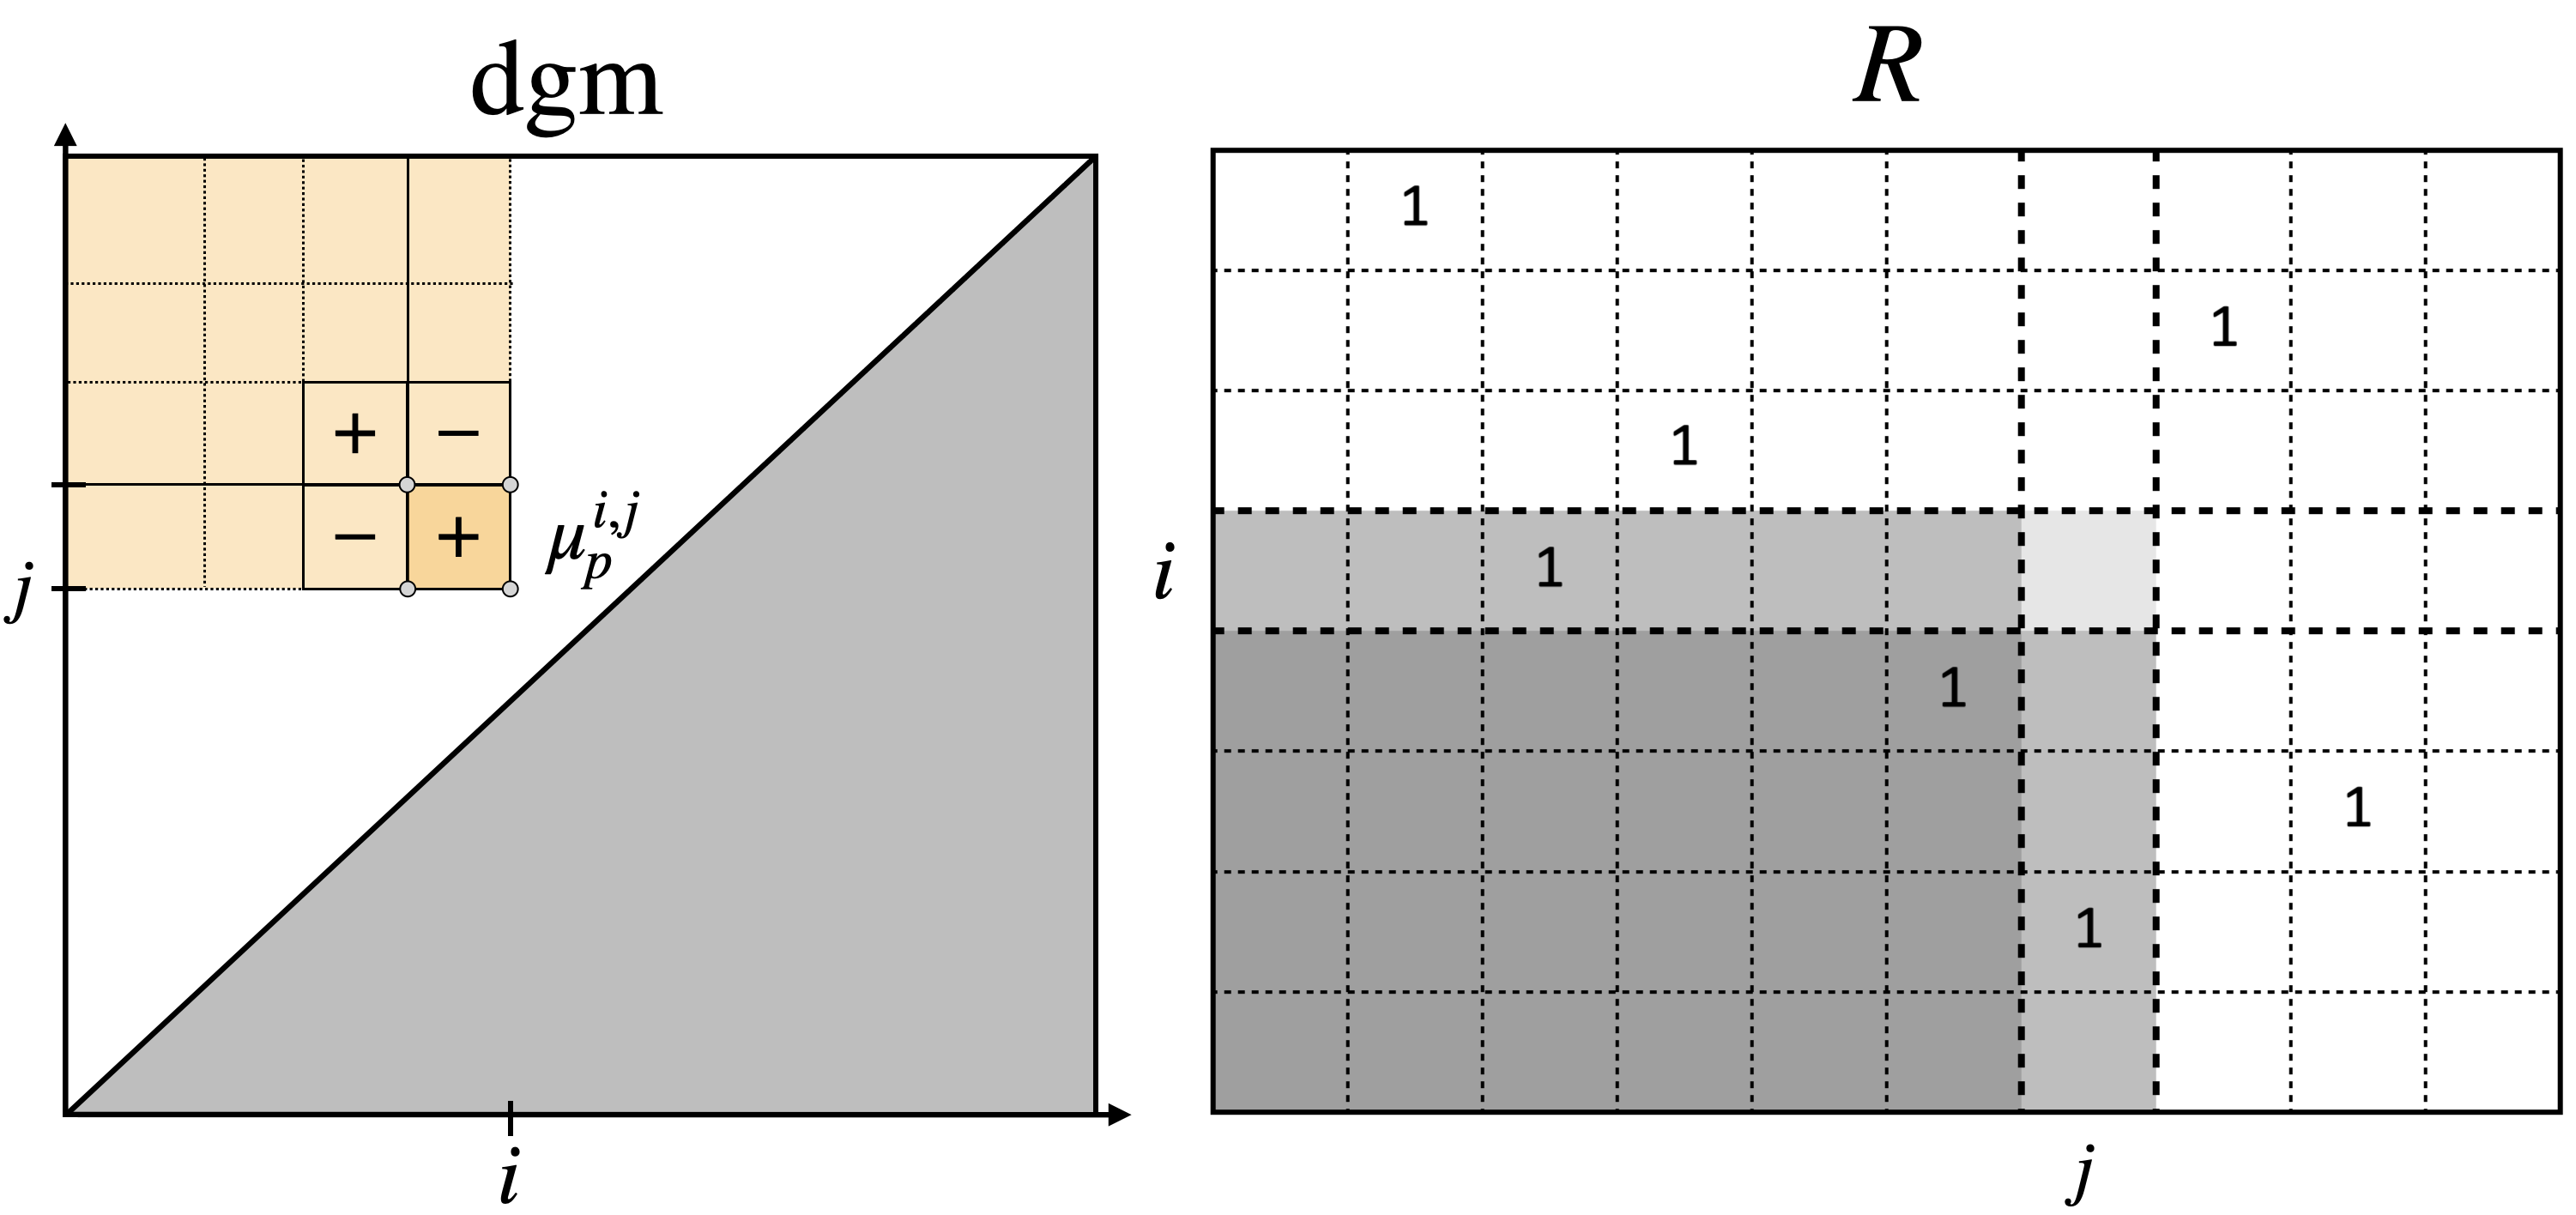
\includegraphics[width=0.45\textwidth]{mult_both}
%	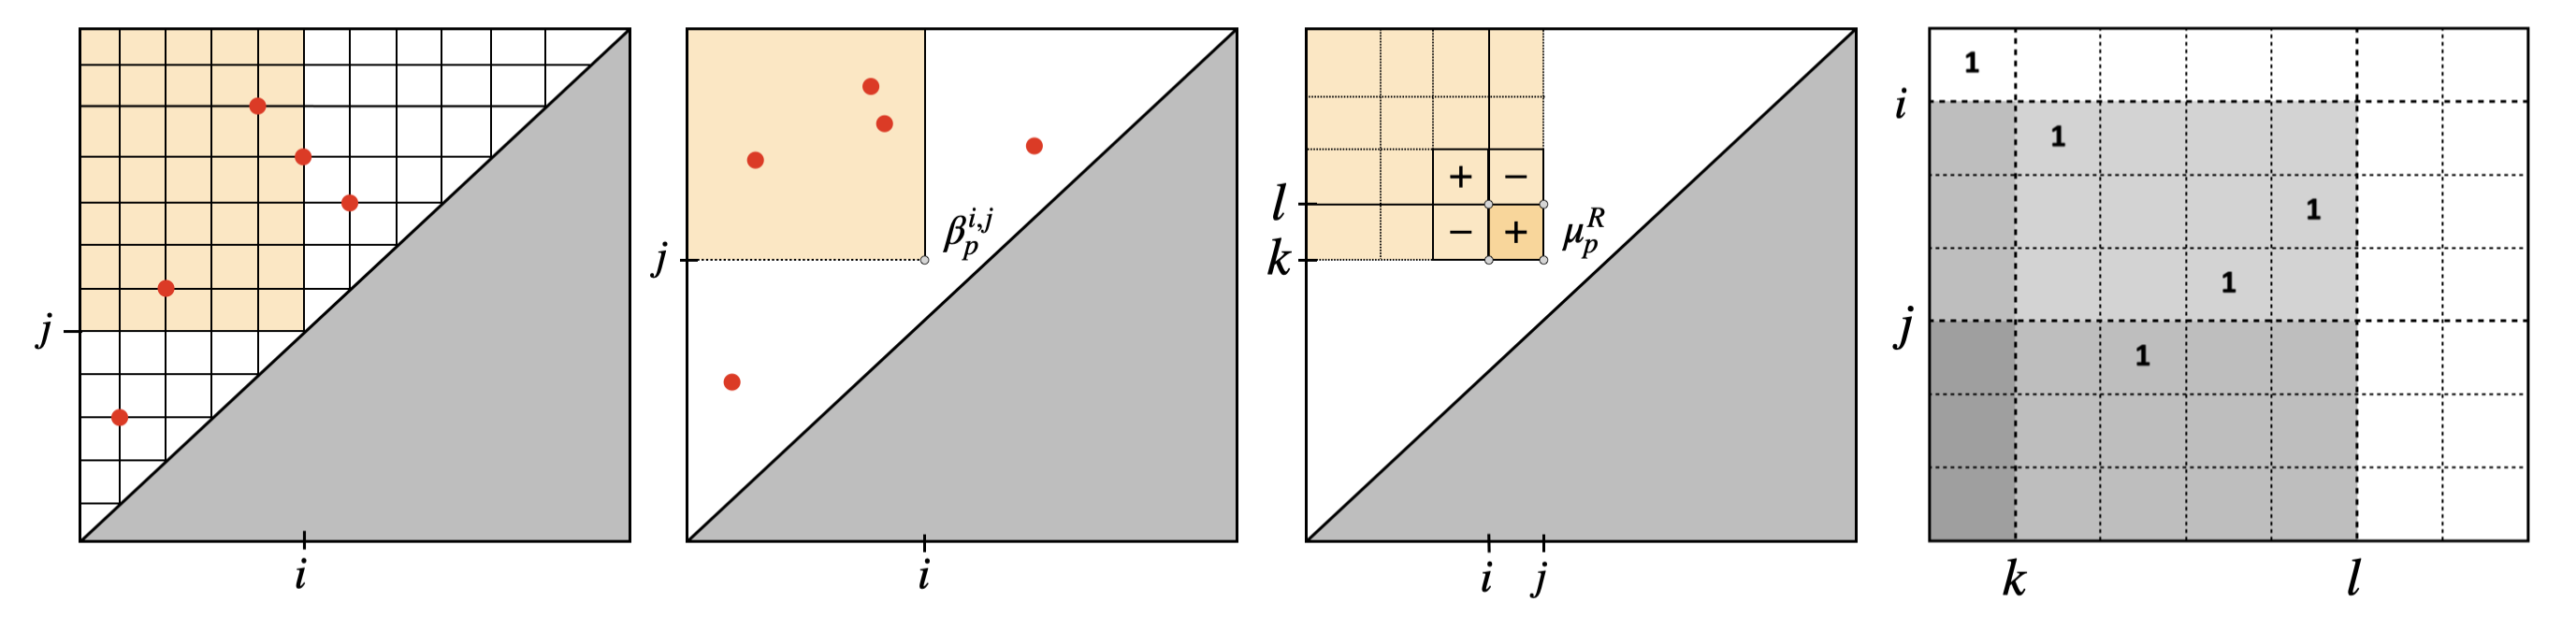
\includegraphics[width=0.85\textwidth]{betti_add}
%	\caption{From left to right, $\beta_p^{i,j}$ counts the number of points (3) in upper left-corner of $\mathrm{dgm}_p(K_\bullet)$, where $(i,j) \in \Delta_+^N$; the same $\beta_p^{\hat\imath, \hat\jmath}$  with $(\hat\imath, \hat\jmath) \in \Delta_+$; the additivity of $\beta_p^{\ast}$ illustrates the form of $\mu_p^{R}$ over $R=[i,j] \times [k,l]$; $\mu_p^R = 4 - 1 - 0 + 0 = 3$ counts pivot entries in the reduced matrix $R = \partial V$ using fact~\eqref{eq:uniq_pivot}.}
%	%$r_R(i,j) = 3 - 2 + 1 - 2 = 0$ yields whether the entry $R[i,j]$ is non-zero.}
%	\label{fig:mult}
%\end{figure}
the corresponding Pairing Uniqueness Lemma~\cite{cohen2006vines} asserts that if $R = \partial V$ decomposes the boundary matrix $\partial \in \mathbb{F}^{N \times N}$ to a \emph{reduced} matrix $R \in \mathbb{F}^{N \times N}$ using left-to-right column operations, then:
%whose lowest non-zero entries satisfy $\mathrm{low}_R(i) \neq \mathrm{low}_R(j)$ whenever both $\mathrm{col}_i(R) \neq 0$ and $\mathrm{col}_j(R) \neq 0$, then:  
\begin{equation}\label{eq:uniq_pivot}
R[i,j] \neq 0 \;\; \Leftrightarrow \;\; \mathrm{rank}(\partial^{i,j}) - \mathrm{rank}(\partial^{i\texttt{+}1,j}) + \mathrm{rank}(\partial^{i\texttt{+}1,j\text{-}1}) - \mathrm{rank}(\partial^{i,j\text{-}1}) \neq 0 
\end{equation}
%where, for any $1 \leq i < j \leq N$, the quantity $r_A(i,j)$ is defined as:
%\begin{equation}
%	r_R(i,j) = \mathrm{rank}(R^{i,j}) - \mathrm{rank}(R^{i\texttt{+}1,j}) + \mathrm{rank}(R^{i\texttt{+}1,j\text{-}1}) - \mathrm{rank}(R^{i,j\text{-}1})
%\end{equation}
where $\partial^{i, j}$ denotes the lower-left submatrix defined by the first $j$ columns and the last $m - i + 1$ rows (rows $i$ through $m$, inclusive). 
Thus, the existence of non-zero ``pivot'' entries in $R$ may be inferred entirely from the ranks of certain submatrices of $\partial$. Part of the validity of~\eqref{eq:uniq_pivot} can be attributed to the following Lemma: 
%the fact that left-to-right elementary column operations, which are known to preserve the ranks of such matrices. 
%As we will use this fact frequently in this paper, we record it formally with a lemma. 
\begin{lemma}\label{lemma:rank}
Given filtration $(K, f)$ of size $N = \lvert K \rvert$, let $R = \partial V$ denote the decomposition of the filtered boundary matrix $\partial \in \mathbb{F}^{N \times N}$. Then, for any pair $(i,j)$ satisfying $1 \leq i < j \leq N$, we have:
	\begin{equation}\label{eq:lower_left_rank}
		\mathrm{rank}(R^{i,j}) = \mathrm{rank}(\partial^{i, j})
	\end{equation}
Equivalently, all lower-left submatrices of $\partial$ have the same rank as their corresponding submatrices in $R$.
\end{lemma} % 
\noindent
%\noindent \textbf{Remark: } Though Lemma~\ref{lemma:rank} is defined over the full boundary matrix $\partial$, there is no loss in generality in its restriction to $p$-dimensional homology exclusively, for any fixed $p \geq 0$. To see this, note that since the reduction algorithm only adds $p$-chains to $p$-chains. Hence, if we set all columns corresponding to simplices of dimension $q \neq p$ to $0$ in the $m \times m$ boundary matrix $\partial$, then $\partial$ recovers the $p$-th boundary operator $\partial_p : C_p(K_\bullet) \to C_{p-1}(K_\bullet)$. 
%In what follows, we will use $\partial_p$ and $R_p$ to refer to matrices of $\partial$ and $R$ whose $q$-chains are set to $0$, for $q \neq p $. 
An explicit proof of both of these facts can be found in~\cite{dey2022computational}, though the latter was also noted in passing by Edelsbrunner~\cite{edelsbrunner2000topological}. 
Though typically viewed as minor facts needed to prove the correctness of the reduction algorithm, the implications of these two observations are are quite general, as recently noted by~\cite{bauer2022keeping}:
\begin{corollary}[Bauer et al.~\cite{bauer2022keeping}]\label{cor:valid_pers}
	Any persistence algorithm which preserves the ranks of the submatrices $\partial^{i,j}(K, f)$ for all $i,j \in [N]$ satisfying $1 \leq i < j \leq N$ is a valid persistence algorithm. 
\end{corollary}

\noindent Indeed, though $R$ is not unique, its non-zero pivots are, and these pivots \emph{define} the persistence diagram. Moreover, due to~\eqref{eq:lower_left_rank}, both $\beta_p^{\ast}$ and $\mu_p^{\ast}$ may be written as a sum of ranks of submatrices of $\partial_p$ and $\partial_{p+1}$:
\begin{corollary}[\cite{chen2011output, dey2022computational}]\label{cor:rank_reduction}
Given a fixed $p \geq 0$, a filtration $(K,f)$ with filtration values $\{ \, a_i \, \}_{i=1}^N$, and a rectangle $R =  [a_i,a_j] \times [a_k,a_l] \subset \Delta_+$,
%satisfying $1 \leq i < j \leq k < l \leq N$, 
the persistent Betti and multiplicity functions may be written as:
	\begin{align*}\label{eq:betti_four}
	% \mathrm{rank}(I_p^{1,i})
	\beta_p^{a_i,a_j}(K,f) &= \mathrm{rank}(C_p(K_i)) - \mathrm{rank}(\partial_p^{1,i}) - \mathrm{rank}(\partial_{p\+1 }^{1,j}) + \mathrm{rank}(\partial_{p\+1}^{i \+ 1, j} ) \numberthis  \\
	\mu_p^{R}(K, f) &= \mathrm{rank}(\partial_{p\+1}^{j \+ 1, k})  - \mathrm{rank}(\partial_{p\+1}^{i \+ 1, k})  - \mathrm{rank}(\partial_{p\+1}^{j \+ 1, l}) + \mathrm{rank}(\partial_{p\+1}^{i \+ 1, l}) \numberthis \label{eq:mu_four}
	%\mathrm{rank}(\partial_{p+1}^{i+1,\ast} \otimes\partial_{p+1}^{\ast,j} )
	\end{align*}
%	where $\lvert K_i^p \rvert$ denotes the number of $p$-simplices in $K_p$. 
%where $I_p^{1,i}$ denotes the first $i$ columns of the $n \times n$ identity matrix.
\end{corollary}
%Dey \& Wang
\noindent Though~\eqref{eq:mu_four} was pointed out by Cohen-Steiner et al. in~\cite{cohen2006vines} and exploited computationally by Chen \& Kerber in~\cite{chen2011output}, to the authors knowledge the only explicit derivation and proof of~\eqref{eq:betti_four} is given by Dey \& Wang~\cite{dey2022computational} (see section 3.3.1). 
For completeness, we give our own detailed proof of corollary~\ref{cor:rank_reduction} in the appendix. 
In practice, neither expressions seem used or even implemented in any commonly used persistence software. 

%If $K$ is finite and $f$ is injective with values $a_j$, ordered, then we can use $\beta_p^{a_i, a_j}(K ,f)$ on the left-hand side of 2.7 and 2.8, and the integers (i,j) on the right. 

%By combining Proposition~\ref{prop:rank_reduction} with~\eqref{eq:dgm}, we recover a submatrix-rank-based $p$-th multiplicity function $\mu_p^{R}(\cdot)$, which to the authors knowledge was first pointed out by Chen \& Kerber~\cite{chen2011output}: 
%\begin{proposition}[Chen \& Kerber~\cite{}]\label{prop:mu_reduction}
%Given a fixed $p \geq 0$, a filtration $K_\bullet = \{K_i\}_{i\in [N]}$ of size $N = \lvert K \rvert$, and a rectangle $R = [i,j] \times [k,l] \subset \Delta_+$,
%%whose indices $(i,j,k,l)$ satisfy $0 \leq i < j \leq k < l \leq N$, 
%the $p$-th multiplicity $\mu_p^{R}$ of $K_\bullet$ is given by:
%	\begin{equation}\label{eq:mu_four}
%	\mu_p^{R}(K_\bullet) = \mathrm{rank}(\partial_{p\+1}^{j \+ 1, k})  - \mathrm{rank}(\partial_{p\+1}^{i \+ 1, k})  - \mathrm{rank}(\partial_{p\+1}^{j \+ 1, l}) + \mathrm{rank}(\partial_{p\+1}^{i \+ 1, l}) 
%	%\mathrm{rank}(\partial_{p+1}^{i+1,\ast} \otimes\partial_{p+1}^{\ast,j} )
%	\end{equation}
%\end{proposition}

% TODO: define beta and mu w.r.t alpha 

%\noindent To gain some intuition of the computational nature of these facts, see Figure~\ref{fig:mult}.
%Note the differences between these two quantities: whereas $\beta_p^{i,j}$ captures points on the diagram that may have unbounded persistence (``essential'' classes~\cite{edelsbrunner2000topological}), the multiplicity function $\mu_p^{R}$ by definition is restricted to classes with bounded persistence\footnote{One may always \emph{cone} the filtration to extend $\mu_p^{R}$ to the unbounded case, see~\cite{chen2011output}}.'

%% Not sure what exactly I want to say here
%For a given $(K, f)$, if $f$ is injective, then every $a_i$ from Corollary~\ref{cor:rank_reduction} will be a homological critical value, as adding a simplex creates or removes a class.  
%it is natural to consider their generalizations under the \emph{persistent measures} setting~\cite{chazal2016structure}.

Two important properties of the expressions from Corollary~\ref{cor:rank_reduction} are: (1) they are comprised strictly of \emph{rank} computations, and (2) all terms involve \emph{unfactored} boundary matrices.
% is that they imply the complexity of obtaining either $\beta_p^{i,j}(K_\bullet)$ or $\mu_p^{R}(K_\bullet)$ may be reduced to the complexity of computing the rank of a set of submatrices of $\partial$---a fact that actually motivated the rank-based persistence algorithm from Chen et al~\cite{chen2011output}.
%Our contributions in this effort stem from the observation that the constitutive terms in these expressions are \emph{unfactored} boundary (sub)matrices---thus, 
Coupled with measure-theoretic perspectives on persistence~\cite{chazal2016structure}, the former suggests variational perspectives of the rank function might yield interesting spectral relaxations of~\eqref{eq:betti_four} and~\eqref{eq:mu_four} useful for e.g. optimization purposes. 
Combined with Corollary~\ref{cor:valid_pers}, the latter property suggests a path to compute persistence information \emph{without} matrix reduction.
%by using e.g. iterative, \emph{matrix-free} approximation schemes 
Moreover, combining these observations suggest advances made in other areas of applied mathematics may be readily exploited, such as the rich theory of matrix functions~\cite{bhatia2013matrix}, the tools developed as part of ``The Laplacian Paradigm''~\cite{teng2010laplacian}, or the recent connections between rank and trace estimation~\cite{ubaru2016fast}.
%with the fact that the rank function is invariant under adjoint transformations with zero-characteristic fields 
%using random matrix theory~\cite{chen2011output}. 
%as opposed to  direct methods that decompose $\partial$ (i.e.~\cite{edelsbrunner2022computational, zomorodian2004computing}).
%The latter fact suggests multiplicity information can be obtained from combination of boundary operators without decomposing or even constructing $\partial$ in memory, enabling the efficient computation of the former using e.g. iterative Krylov or subspace acceleration methods~\cite{golub2013matrix, parlett1994we}. 
%Moreover, the measure-theoretic counter-parts~\eqref{eq:pbn_cont} and~\eqref{eq:measure} suggests we may re-use  
%may be exploited to accelerate the computation further. 
%the structure of $\partial \cdot \partial^T$, 
%---such as invariance under permutations and adjoint multiplication---
%may lead to interesting overlap in other popular areas of applied mathematics, such as compressive sensing, 
%By working with persistence modules indexed with real-valued coefficients, we naturally recover the measure-theoretic perspective from~\eqref{eq:measure}.
The rest of the paper is dedicated to exploring these connections and their implications. 

%\begin{remark}
%% Change index set
%We have thus far used integer indices $(\,i, j\,) \in \Delta_+^N$ to describe persistent quantities over a filtration $K_\bullet = (K, f)$ of size $\lvert K \rvert = N$, which is equivalent to filtering $K$ over the index set $f : K \to [N]$.
%It is more common in practice to define persistence of a persistent-pair $(f(\sigma_i),f(\sigma_j)) \in \mathrm{dgm}(K_\bullet)$ via $f(\sigma_j) - f(\tau_i)$, rather than as $j - i$, especially when $f$ is  geometric in nature.
%%For example, when $f : K \to \mathbb{R}$ satisfies $f(\sigma') \leq f(\sigma)$ for every $\sigma' \subseteq \sigma$, the subcomplexes $K_i = f^{-1}(-\infty, \hat\imath \,]$ of $K$ represent sublevel sets $f^{-1}(-\infty, \hat\imath \,]$ for every $\hat\imath \in \mathbb{R}$. 
%In this setting, each pair $(i,j) \in \mathrm{dgm}(K_\bullet)$ is typically represented as the point $(\, \hat\imath, \hat\jmath \, )$ where $\hat\imath = f(\sigma_i)$ and $\hat\jmath = f(\sigma_j)$.
%% In theory, any function satisfying $f(\tau) \subseteq f(\sigma)$ for every face/coface pair $(\tau, \sigma)$ yields a well defined persistence diagram. 
%%Unless it is clear from the context, we alter our notation by re-defining $\beta_p^{\hat\imath,\hat\jmath}$ using pairs $(\,\hat\imath,\hat\jmath\,) \in \Delta_{+}$ from the upper-half plane $\Delta_{+} = \{ \, (x,y) \in \mathbb{R}^2 : y > x \, \} $ for the remainder of the paper.
%%Since this is equivalent to reindexing a given filter $f : K \to \mathbb{R}$ over the index set $[N]$, 
%%Since persistence diagrams are isomorphic under monotone transformations of the index set, 
%For simplicity of notation, we will exploit the inclusion-exclusion property of persistence measures~\cite{chazal2016structure} by continuing to use the notation $(\,i, j\,)$ to denote pairs $(\,i, j\,) \in \Delta_{+}$ from the upper-half plane $\Delta_{+} = \{ \, (x,y) \in \mathbb{R}^2 : y > x \, \} $.
%\end{remark}

%In contrast to the persistence diagram, note that both of counting invariants are neither stable nor smooth as they are integer-valued quantities.
%However, as~\eqref{eq:mu_four} makes clear, the restriction to sub-matrices is akin to computing $R$-parameterized multiplicities over the index-persistence plane $\Delta_+^N$. 
%Moreover, suppose we: 
%\begin{enumerate}
%	\item Restrict ourselves to $H_p(K; \mathbb{R})$
%	\item Index $K_\bullet$ over the (real) upper-half plane $\Delta_+$
%	\item Parameterize the chains $C_p(K_\bullet; \mathbb{R})$ with real-valued entries
%\end{enumerate}


%We exploit various properties of the rank function to 
%Using various properties of the rank function, this accelerate the computation of both invariants. 
%Combined with various properties of the rank function, we exploit this aspect of to accelerate the computation of both invariants in~\eqref{eq:betti_four} and~\eqref{eq:mu_four}. 

%To get some intuition on what the structure and size of these matrices, we include a picture of each of the terms in Equation~\eqref{eq:betti_four}. 
%\begin{figure}[!h]
%	\centering
%	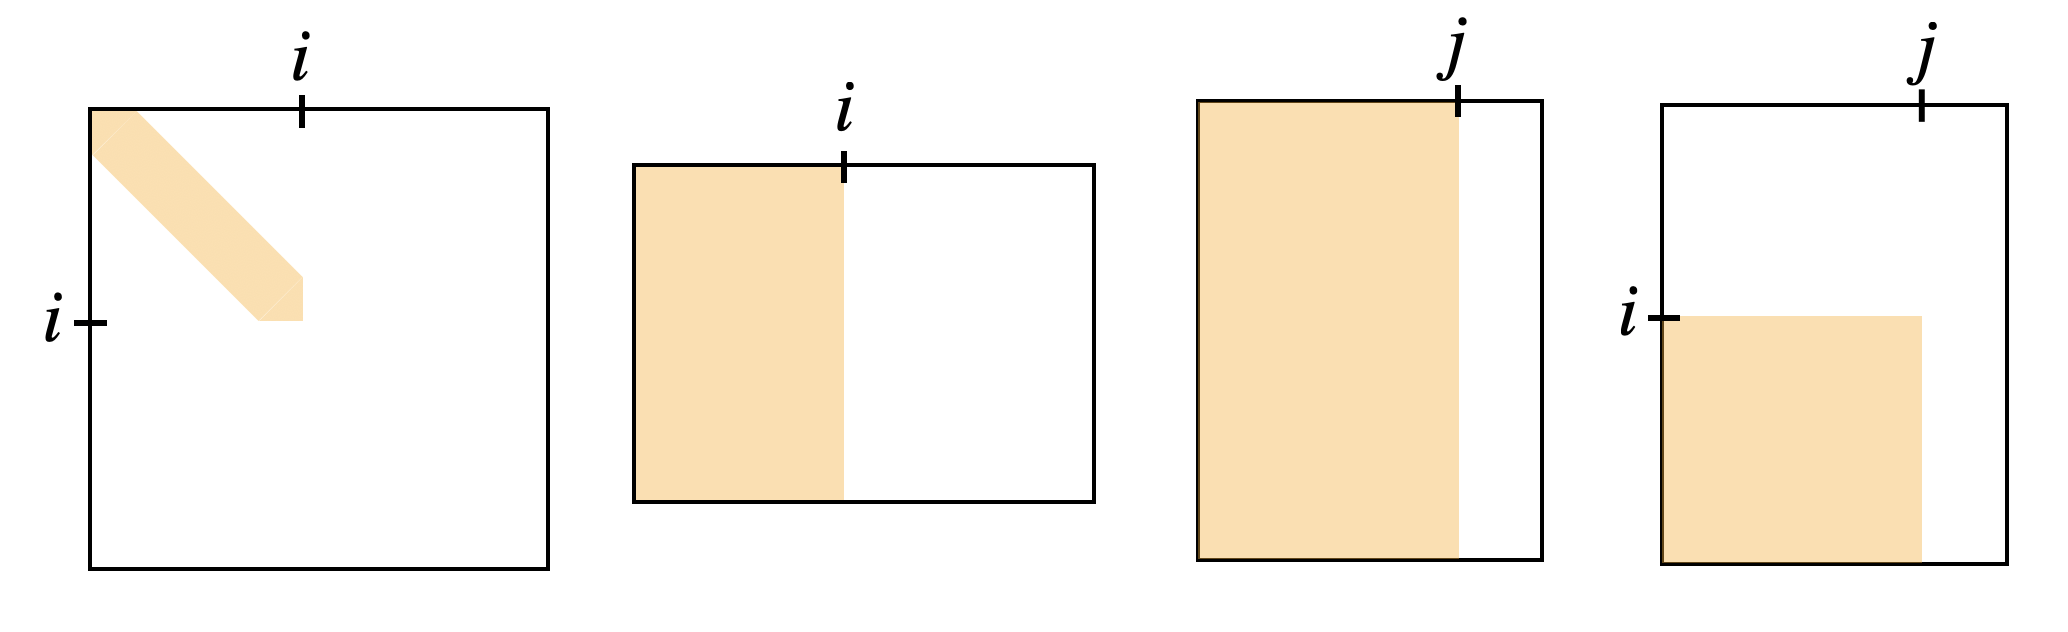
\includegraphics[width=0.70\textwidth]{four_matrices}
%	\caption{The four matrices whose ranks yield $\beta_p^{i,j}$ in the same order as given in~\eqref{eq:betti_four}. Each solid portion represents (sparse) blocks of non-zero entries, while each white portion is zero. Observe $\partial_{p+1}^{i+1, j} \subseteq \partial_{p+1}^{1,j}$ can be obtained by intersecting the non-zero entries of $\partial_{p+1}^{1,j}$ with the non-zero entries in the complement of $\partial_p^{1,i}$.  }
%\end{figure}
%Boundary matrices are sparse and highly structured: given $K_\bullet$ with $m$ simplices $\sigma_1, \sigma_2, \dots, \sigma_m$ constructed from a $p$-dimensional complex $K$, its full boundary matrix $\partial$ is upper-triangular and has a storage complexity of: 
%\begin{equation}
%	\mathrm{nnz}(\partial) \sim O(m \log m)
%\end{equation} 
%To see this, note that since a $p$-simplex has $2^{p+1} - 1$ faces, we have $p \leq \log(m + 1) - 1$. Moreover, since each column of $\partial_p^\ast$ contains exactly $p+1$ non-zero entries, $\mathrm{nnz}(\partial) \sim O((p+1)m)$.


%\begin{proposition}\label{prop:mu_query}
%For any fixed $p \geq 0$, let $\partial_p$ denote the $p$-dimensional boundary matrices of filtration $K_\bullet$ of size $n = \lvert K^{(p)} \rvert$, $m = \lvert K^{(p\+1)} \rvert$.
%Let $R = [i,j] \times [k,l]$ denote a fixed rectangle in $\mathbb{R}^2$ satisfying $a < b \leq c < d$. The multiplicity $\mu_p^R$ of this box is given by:
%	\begin{equation}\label{eq:mu_four}
%	\mu_p^{R} =  \mathrm{rank}(\partial_{p\+1}^{j} ) - \mathrm{rank}(\partial_{p\+1}^{i \+ 1, j} )
%	%\mathrm{rank}(\partial_{p+1}^{i+1,\ast} \otimes\partial_{p+1}^{\ast,j} )
%	\end{equation}
%where $I_p^{1,i}$ denotes the first $i$ columns of the $n \times n$ identity matrix.
%\end{proposition}
%\begin{corollary}
%	Given a filtration $K_\bullet$ of size $n = \lvert K_{i}^{(p)} \rvert$ and $m = \lvert K_{j}^{(p+1)} \rvert$ and two indices $i \in [n]$, $j \in [m]$, computing $\beta_p^{i,j}$ can be done in time and storage complexity $O(\max \{\, R_\partial(n, i, p), \, R_\partial(m, j, p+1) \,\})$ where $R_\partial(a,b,c)$ is the complexity of computing the rank of a $c$-dimensional $a\times b$ boundary matrix with $b\cdot (c+1)$ non-zero $\mathbb{F}$ entries. 
%	%with $n < m$
%\end{corollary} 

% --- Generic Rank approximation via eigenvalues --- 
\section{Spectral relaxation and its implications}\label{sec:spectral_sec}
%The following derivations of the persistent Betti number will be used in proofs and serve as the primary technical motivations for this effort.
%To begin introducing our proposed relaxation, we successively  relaxing and generalizing different aspects of~\eqref{eq:betti_four}. 
Prior to introducing our proposed relaxation, it is instructive to examine the how traditional expressions of the persistent rank invariants compare to  those from Corollary~\ref{cor:rank_reduction}. 
Given a filtration $(K,f)$ of size $N = \lvert K\rvert$ with $f: K \to I$ defined over some index set $I$, its $p$-th persistent Betti number $\beta_p^{a,b}$ at index $(a,b) \in I \times I$, is defined as follows: 
\begin{align*} \label{eq:pbn}
	\centering
	\beta_p^{a,b } &= \mathrm{dim} \left ( Z_p(K_a) / B_p(K_b) \right ) \\
	& = \mathrm{dim} \left( Z_p(K_a) / (Z_p(K_a) \cap B_p(K_b) \right) \\
	& \numberthis = \mathrm{dim} \left( Z_p(K_a) \right) - \mathrm{dim}\left( Z_p(K_a) \cap B_p(K_b) \right ) 
\end{align*}
%As the multiplicity function $\mu_p^R$ can be written~
%By definition, the boundary and cycle groups $B_p(K_b)$ and $Z_p(K_a)$ are subspaces of the operators $\partial_p(K_a)$ and $\partial_{p+1}(K_b)$, yielding the following two-term expression: 
%\begin{equation}\label{eq:pbn_simple}
%	\beta_p^{a,b} = \mathrm{dim}\big( \; \mathrm{Ker}(\partial_p(K_a)) \; \big) - \mathrm{dim}\big( \; \mathrm{Ker}(\partial_p(K_a)) \cap \mathrm{Im}(\partial_{p+1}(K_b)) \; \big) 
%\end{equation}
Computationally, observe that~\eqref{eq:pbn} reduces to one nullity computation and one subspace intersection computation. % via matrix reduction or projector-based techniques 
While the former is easy to re-cast as a spectral computation, computing the latter typically requires obtaining bases via matrix decomposition. Constructing these bases explicitly using conventional~\cite{bhatia2013matrix, golub2013matrix} or persistence-based~\cite{memoli2022persistent, zomorodian2004computing} algorithms effectively\footnote{Note about matrix multiplication constant} requires $\Omega(N^3)$ time and $\Omega(N^2)$ space.
As the persistence algorithm also exhibits $O(N^3)$ time complexity and completely characterizes $\beta_p^{a,b}$ over \emph{all} values $(a,b) \in I \times I$, there is little incentive to compute $\beta_p^{a,b}$ with such direct methods (and indeed, they are largely unused). Because of this, we will focus on expressions~\eqref{eq:betti_four} and~\eqref{eq:mu_four} throughout the rest of the paper.
%or they involve forming orthogonal projectors
%re are both general-purpose~\cite{bhatia2013matrix, golub2013matrix} and persistence-specific algorithms to compute.
% Moreover, all of these methods have been shown to 
%Specializations of these direct methods to filtered simplicial complexes have proven challenging to efficiently extend to the parameterized setting~\cite{piekenbrock2021move}, prompting questions of whether alternative derivations (e.g.~\eqref{eq:mu_four}) exhibit different computational characteristics.

%$\mathrm{dim}\big(\mathrm{Ker}(\partial_p(K_i))\big) = \mathrm{nullity}(\partial_p(K_i))$
%Since the nullity of an operator may be reduced to a rank computation via rank-nullity, the complexity of first term may be reduced to the complexity of computing the rank of a sparse $n \times m$ matrix. 
%In contrast, the persistence term 

% This subsection shows the benefits of rank(P^T A P) = rank(A)
\subsection{Parameterized boundary operators}\label{sec:param_boundary}
%As stated in section~\ref{sec:intro}, we are concerned with the computation of certain topological invariants in \emph{parameterized} settings, i.e. settings where the input data---geometrically realized as simplicial complexes---is thought to be generated from a parameterized family. Such families naturally arise in many applications, e.g. in Rips filtrations parameterized by dynamic metric spaces~\cite{} or in multi-parameter persistence settings~\cite{}.  
%Though the boundary matrices in~\eqref{eq:betti_four} are given in filtration order to preserve the inclusion relations between simplices in $K_\bullet$, the permutation invariance of the rank function suggests $\partial$ need not be ordered at all to be evaluated---so long as each constitutive term has the same non-zero pattern as its filtration-ordered counterpart, their ranks will be identical.
%% Another approach to tracking the PBNs in parameterized setting is to maintain a persistence diagram through the vineyards algorithm~\cite{cohen2006vines}. This, however, requires $O(m^2)$ memory and an $\approx O(m^2)$ preprocessing procedure to detect changes in the filtration order\footnote{The bound $O(m^2)$ assumes the homotopy changes each filtration value monotonically throughout the homotopy. Otherwise the number of order changes is clearly unbounded.} to simulate persistence across a homotopy, the canonical continuous parameterized setting. In contrast, as we show below, PBNs need no such preprocessing procedure and may be computed in effectively $O(m)$ memory, even in parameterized settings. 
%Recall that the boundary operator $\partial_p$ for a filtration pair $(K_{\bullet}, f)$ of size $m = \lvert K \rvert$ is represented by an ordered $(m \times m)$ boundary matrix $\partial_p$ whose columns and rows corresponding to $q$-simplices and $(q-1)$-simplices are zero, for $q \neq p$.
%After orienting $K$ in an arbitrary but consistent way, the entries of $\partial_p$ have the form: 
%\begin{equation}\label{eq:matrix_pchain}
%	\partial_p[k, l] = \begin{cases} 
%	c(\sigma_j)  & \text{if } \sigma_l \in \partial_p(\sigma_k) \\
%	0 & \text{otherwise}
%   \end{cases}
%\end{equation}
%where $c(\sigma_\ast) \in \mathbb{F}$ is an arbitrary constant satisfying $c(\sigma) = -c(\sigma')$ if $\sigma$ and $\sigma'$ are opposite orientations of the same simplex, typically set to $\pm 1$. In what follows, we assume a fixed orientation is given on $K$, and write $\pm c(\sigma)$ to indicate the sign of $c(\sigma)$ depends on the orientation of $\sigma$. Note that, for the reduction algorithm, the ordering of $\partial_p$ must respect the facet poset of $K_\bullet$: if $\tau, \sigma \in K_\bullet^{(p)}$ and $f(\tau) \leq f(\sigma)$, then the chain $\partial_p(\tau)$ must appear before $\partial_p(\sigma)$ in $\partial_p$. %such that the elementary left-to-right matrix operations. 
%such that $\mathrm{range}(f) = \mathbb{R}$, and it is often more informative to work with the pairs $(f(\tau_i), f(\sigma_j))$ stemming from the persistent-pairs $()$ persistence diagram 
% A common scenario is where $K_\bullet$ is obtained via a Rips filtration constructed over a metric space $(X, d_X)$. In this case $f : \mathcal{P}(X) \to \mathbb{R}_+$ is given as the diameter $f(\sigma) = \max_{x,x' \in \sigma} d_X(x,x')$. 
% mention DMSs 
%In many applications it is of interest to study such filter function in parameterized settings, e.g. given some set of parameters $\mathcal{H}$, the goal is to understand a given topological invariant at many  parameters $h \in \mathcal{H}$, i.e. treat $f : \mathcal{P}(X) \times \mathcal{H} \to \mathbb{R}_+$. We include several example in section~\ref{}.
%To see the utility of this fact, consider a filtration $(K_\bullet, f)$ equipped with a \emph{parameterized} filter function $f : \mathcal{A} \times K \to \mathbb{R}$ with respect to some set $\mathcal{A}$.
In typical dynamic persistence settings (e.g.~\cite{cohen2006vines}), a decomposition $R = \partial V$ of the boundary matrix $\partial$ must be permuted and modified frequently to maintain a simplexwise order respecting $f_\alpha$.  %$P R P^T = (P \partial P^T)(P V P^T)$
In contrast, one benefit of the rank function is its permutation invariance: for any $X \in \mathbb{R}^{n \times n}$ and permutation $P$ we have: 
$$ \mathrm{rank}(X) = \mathrm{rank}(P^T X  P) $$
%There are computational advantages to the lesser known rank invariant expressions~\eqref{eq:betti_four} and~\eqref{eq:mu_four} due to the many invariances of the rank function. One such property is permutation invariance: given any $A \in \mathbb{R}^{n \times n}$, it is easy to see that $\mathrm{rank}(A) = \mathrm{rank}(P^T A P)$ for any permutation matrix $P$.  
% In contrast, the permutation invariance of the rank function suggests $\partial$
This suggests persistent rank computations like those from Corollary~\ref{cor:rank_reduction} need not maintain this ordering---as long as the constitutive boundary matrices the same non-zero pattern as their filtered counterparts, their ranks will be identical.
%In this section, we exploit this fact by showing how~\eqref{eq:betti_four} and~\eqref{eq:mu_four} may be made \emph{continuously parameterized}.
In what follows, we demonstrate how exploiting this permutation invariance significantly simplifies the practical use of~\eqref{eq:betti_four} and~\eqref{eq:mu_four} in \emph{parameterized} settings. 

%Permutation invariance is a useful property for computation in parameterized setting. 
%\begin{definition}[Parameterized $\partial_p$]\label{def:time_boundary_matrix}
Let $(K, f_\alpha)$ denote parameterized family of filtrations of a simplicial complex of size $\lvert K^p \rvert = n$. Fix an arbitrary linear extension $(K, \preceq)$ of the face poset of $K$. 
Define the $\mathcal{A}$-\emph{parameterized} \emph{boundary operator} $\hat{\partial}_p(\alpha) \in \mathbb{R}^{n \times n}$ of $(K, f_\alpha)$ as the $n \times n$ matrix ordered by $\preceq$ for all $\alpha \in \mathcal{A}$ whose entries $(k,l)$ satisfy:
\begin{equation}\label{eq:param_boundary_matrix}
	\partial_p(\alpha)[k,l] = \begin{cases}
	% \pm \, S_{i,j}(\sigma_k, \sigma_l) & \text{if } \sigma_k \in \partial_p(\sigma_l) \\
s_{kl} \cdot f_\alpha(\sigma_k) \cdot f_\alpha(\sigma_l) & \text{if } \sigma_k \in \partial_p(\sigma_l)\\
%	s_{kl} \cdot (\bar{S}_{i} \circ f_h)(\sigma_k)^+ \cdot (S_{j} \circ f_h)(\sigma_l) & \text{if } \sigma_k \in \partial_p(\sigma_l)\\
	%, \text{ where } \epsilon = f(\sigma_l) \\
	0 & \text{otherwise}
\end{cases}
\end{equation}
%where $S_{i} : \mathbb{R} \to \{0, 1\}$ is a \emph{step} function satisfying $S_i(x) = 0$ if $x > i$ and $1$ otherwise, $\bar{S}_{i} = 1 - S_i$, $f_h(\sigma) = f(\sigma, h)$, 
where $s_{kl} = \mathrm{sgn}([\sigma_k], \partial [\sigma_l])$ is the sign of the oriented face $[\sigma_k]$ in $\partial[\sigma_l]$.
% and the quantity $x^{+} = x^{-1}$ if $x > 0$ and $0$ otherwise.
%\end{definition}
\noindent
Observe that $\partial_p(\alpha)$ may be decoupled~\eqref{eq:param_boundary_matrix} into a product of diagonal matrices $D_\ast(f_\alpha)$: 
	\begin{equation}\label{eq:decouple}
		\partial_p(\alpha) \triangleq D_p(f_\alpha) \cdot \partial_p(K_\preceq) \cdot D_{p+1}(f_\alpha) 
	\end{equation}
	where $D_p(f_\alpha)$ and  $D_{p+1}(f_\alpha)$ are diagonal matrices whose non-zero entries are ordered by restrictions of $f_\alpha$ to $K_\preceq^p$ and $K_\preceq^{p+1}$, respectively.
	%based on restrictions of $f_\alpha$ to $K^p$ and $K^{p+1}$, respectively.
%We refer to the fixed inner matrix $\partial_p \in \{-1, 0, 1\}^{n \times m}$ as the \emph{sign pattern matrix}.
Clearly, $\mathrm{rank}(\partial_p(\alpha)) = \mathrm{rank}(\partial_p(K_\preceq))$ when the diagonal entries of $D_p$ and $D_{p+1}$ are strictly positive. Moreover, observe we may restrict to those ``lower left'' matrices from Lemma~\ref{lemma:rank} via post-composing step functions $\bar{S}_a(x) = \mathbbm{1}_{x > a}(x)$ and $S_b(x) = \mathbbm{1}_{x \leq b}(x)$ to $D_p$ and $D_{p+1}$, respectively:
\begin{equation}\label{eq:rank_equiv_param}
%	\mathrm{rank}(\, \partial_p^{i,j}(K_\bullet) \, ) = 
	 \hat{\partial}_p^{a,b}(\alpha) \triangleq D_p(\bar{S}_a \circ f_\alpha) \cdot \partial_p(K_\preceq) \cdot D_{p+1}(S_b \circ f_\alpha) 
	\end{equation}
%where $\bar{S}, S : \mathbb{R} \to \{0,1\}$ are up and down step functions, respectively,.
%\begin{equation}\label{eq:step_functions}
%	\bar{S}_i(x) = \begin{cases} 1 & \text{if } x > i \\ 0 & \text{otherwise}\end{cases}, \quad \quad S_j(x) = \begin{cases} 1 & \text{if } x \leq j \\ 0 & \text{otherwise}\end{cases}
%\end{equation}
% TODO: maybe mention relative chains
Though these step functions are discontinuous at their chosen thresholds $a$ and $b$, we may retain the element-wise continuity of~\eqref{eq:decouple} by exchanging them with clamped \emph{smoothstep} functions $\mathcal{S}: \mathbb{R} \to [0, 1]$ that interpolate the discontinuous step portion of $S$ along a fixed interval $(a,a+\omega)$, for some $\omega > 0$ (see Figure~\ref{fig:smoothstep}).
%of the form: 
%In particular, we swap out the step functions $S : \mathbb{R} \to \{ 0, 1\}$ from~\eqref{eq:param_boundary_matrix} with \emph{smoothstep} functions $\mathcal{S}: \mathbb{R} \to [0, 1]$. 
%\begin{equation}\label{eq:smoothstep}
%\mathcal{S}_a^{\omega} (x) = \begin{cases}
%	0 & x \leq a \\
%	P_n\big( \omega^{-1}((a + \omega) - x) \big) & a < x < a + \omega \\
%	1 & a + \omega \leq x
%\end{cases}
%\end{equation} 
%where $P_n: [0,1] \to [0,1]$ is a $n$-th order polynomial satisfying $P_n(0) = 0$ and $P_n(1) = 1$.

%\\
%\\
%\noindent To adapt these relaxations to the rank expressions given in Proposition~\ref{prop:mu_betti_1}, we need to modify the boundary chains in~\eqref{eq:alt_sum} to vary continuously in $\mathcal{A}$, which remain discontinuous due to the use of step functions~\eqref{eq:step_functions}.

The observations above collectively motivate our first relaxation. Without loss in generality, assume the orientation of the simplices $(K, \preceq)$ is induced by the order on the vertex set $V$. To simplify the notation, we write $A^{x} = A^{\ast,x}$ to denote the submatrix including all rows of $A$ and all columns of $A$ up to $x$. 
%We also write $r(A) = \mathrm{rank}(A)$.
% TODO: ask Jose about this
%We also use $\mathcal{K}_f$ to denote the space of all filtration pairs $(K, f)$.
\begin{proposition}\label{prop:mu_betti_1}
	Given $(K, f_\alpha)$, any rectangle $R = [a,b] \times [c,d] \subset \Delta_{+}$, and $\delta > 0$ the number satisfying $a + \delta < b - \delta$ from~\eqref{eq:measure}
	%satisfying $i < j \leq k < l$, 
	the $\mathcal{A}$-parameterized invariants $\beta_p^{a,b} : \mathcal{A} \times K \to \mathbb{N}$ and $\mu_p^{R} : \mathcal{A} \times K \to \mathbb{N}$ defined by: 
	\begin{align*}\label{eq:pbn_parameterized}
%	\lvert K_a^{p}(\alpha) \rvert 
		\beta_p^{a,b}(\alpha) &\triangleq \mathrm{rank}\big(D_p(S_a \circ f_\alpha)\big) - \mathrm{rank}\big(\,\hat{\partial}_{p}^{a}(\alpha)\,\big) - \mathrm{rank}\big(\,\hat{\partial}_{p+1}^{b}(\alpha)\,\big) + \mathrm{rank}\big(\,\hat{\partial}_{p+1}^{a \+ \delta, b}(\alpha)\,\big) \numberthis \\
%	\end{align*}
%	\vspace{-2.1em}
%	\begin{align*}
	\mu_p^{R}(\alpha) &\triangleq \mathrm{rank}\big(\, \hat{\partial}_{p+1}^{b \+ \delta, c}(\alpha)\,\big) - \mathrm{rank}\big(\, \hat{\partial}_{p+1}^{a \+ \delta, c}(\alpha)\,\big) - \mathrm{rank}\big(\, \hat{\partial}_{p+1}^{b \+ \delta, d}(\alpha)\,\big) + \mathrm{rank}\big(\, \hat{\partial}_{p+1}^{a \+ \delta, d}(\alpha)\,\big) \numberthis \label{eq:mu_parameterized}
	\end{align*}
	yield the correct quantities $\mu_p^R(K, f_\alpha) = \mathrm{card} \left( \, \restr{\mathrm{dgm}_p(f_\alpha)}{R} \, \right)$ and $\beta_p^{a,b} = \mathrm{dim}(H_p^{a,b}(K, f_\alpha))$ for all $\alpha \in \mathcal{A}$. 
%	Moreover, if $f_\alpha$ is Lipshitz continuous in $\alpha$ and the step functions $S_\ast$ are replaced by smoothstep functions $\mathcal{S}_\ast$, then the non-zero entries $\hat{\partial}_{p+1}^{\ast}[i,j]$ of $\hat{\partial}_{p+1}^{\ast}$ are also Lipshitz in $\alpha \in \mathbb{R}$. 
%	Moreover, the entries of $\hat{\partial}_p^\ast(\alpha)$ vary continuously in $\mathcal{A}$.
\end{proposition}
\noindent For completeness, a proof of Proposition~\ref{prop:mu_betti_1} is given in the appendix. 
%\begin{remark}
Note that in~\eqref{eq:rank_equiv_param}, we write $\partial_p(K_{\preceq})$ (as opposed to $\partial_p(K, f)$) to emphasize $\partial_p(K_{\preceq})$ is ordered  according to a fixed linear ordering $(K, \preceq)$. The distinction is necessary as evaluating the boundary terms from corollary~\ref{cor:rank_reduction} would require $\partial$ to be explicitly filtered in the total ordering induced by $f_\alpha$---which varies in $\mathcal{A}$---whereas the expressions obtained by replacing the constitutive terms in~\eqref{eq:betti_four} and~\eqref{eq:mu_four} with~\eqref{eq:pbn_parameterized} and~\eqref{eq:mu_parameterized}, respectively, require no such explicit filtering.  
%permutation invariant in $\mathcal{A}$. 
%\end{remark}
%To 
\begin{corollary}
	Given a boundary matrix $\hat{\partial}_p(\alpha) \in \mathbb{R}^{n \times n}$ constructed at time $\alpha \in \mathbb{R}$ from a parameterized family of filtrations $(K, f_\alpha)$ with linear extension $\preceq$, 
	the time complexity of constructing $\hat{\partial}_p(\alpha')$ for any other $\alpha' \neq \alpha$ is $O(\mathrm{max}(\lvert K^p \rvert, \lvert K^{p+1} \rvert))$, assuming the evaluation of $f_\alpha(\tau)$ is $O(1)$ for every simplex $\tau \in K$.  
	
%	 Let $\hat{\partial}_p = \hat{\partial}_p^{-\infty, \infty}$ denote the full boundary matrix constructed from a fixed simplexwise filtered simplicial complex $(K, \preceq)$. add linear-time complexity result related to considering sub-complexes at varying $\alpha \neq \alpha'$. 
	% TODO: add a remark about how constructing boundary matrices / complexes in general is often the bottleneck  
\end{corollary}

%Thus we may solve this problem by solving $n$ sparse linear systems of that take the form $Ax = b$, where here $A$ is a Laplacian matrix with an $\epsilon \cdot I_n$ addition to it's diagonal. 
\subsection{Parameterized Laplacians}\label{sec:laplacian_theory2}
 For generality's sake, it is important to make the class of expressions for $\beta_p^\ast$ and $\mu_p^\ast$ as large as possible.
%elucidate the necessary conditions under which the spectral operators from section~\ref{sec:spectral_relax} are differentiable, so as to make the class of such operators as large as possible. 
%Towards this, we exploit another identity of the rank function applicable to zero-characteristic fields $\mathbb{F}$:
Since we are only concerned with homology over $\mathbb{R}$, we may exploit another identity of the rank function which is only applicable to zero characteristic fields: 
%$$\mathrm{rank}(\partial_p) = \mathrm{rank}(\partial_p \circ \partial_p^T) = \mathrm{rank}(\partial_p^T \circ \partial_p)$$ 
$$\mathrm{rank}(X) = \mathrm{rank}(X X^T) = \mathrm{rank}(X^T X), \quad \text{for all } X \in \mathbb{F}^{n \times m}$$ 
% study of spectra of \emph{combinatorial Laplacians}
In the context of boundary operators, note that $\partial_1 \partial_1^T$ is the well known \emph{graph Laplacian}~\cite{chung1997spectral}, indicating we may express $\beta_0^\ast(\alpha)$ and $\mu_0^\ast(\alpha)$ using the ranks of Laplacian\footnote{By convention, we define $\partial_p = 0$ for all $p \leq 0$.} matrices.
%Indeed, as the eigenvalues of $XX^T$ (or $X^T X$) are given by the squares of the singular values of $X$, we may study the singular values of boundary operators through the spectra of Laplacians.  

Following the seminal results from Horuk and Jost~\cite{horak2013spectra}, there are three natural ways to define ($p$-) Laplacian operators over a fixed simplicial complex $K$: the \emph{up}-Laplacian $L_p^{\text{up}}(K)$, the \emph{down}-Laplacian $L_p^{\text{dn}}(K)$, and their sum, which we refer to as the \emph{combinatorial} Laplacian $\Delta_p(K)$: 
\begin{equation}\label{eq:comb_lap}
	\Delta_p = \underbrace{\partial_{p\+1} \circ \partial_{p\+1}^T}_{L_p^{\text{up}}} + \underbrace{\partial_{p}^T  \circ  \partial_{p}}_{L_p^{\text{dn}}} 
%	\simeq H() 
\end{equation}
\noindent 
All three operators $\Delta_p$, $L_p^{\text{up}}$, and $L_p^{\text{dn}}$ are symmetric, positive semi-definite, and compact~\cite{memoli2022persistent}---moreover, the \emph{non-zero} multisets $\Lambda(L_p^{\text{up}})$ and $\Lambda(L_{p+1}^{\text{dn}})$ are equivalent, implying they must have identical ranks (see Theorem 2.2 and 3.1 of~\cite{horak2013spectra}). 
%and thus have real, non-negative eigenvalues
Thus, for rank computations, it suffices to consider only one of them.
%Thus, from a rank-based perspective, any of these operators may be readily substituted for $\hat{\partial}_p^\ast$ in Proposition~\ref{prop:mu_betti_1}.

%moreover, as shown by~\cite{horak2013spectra}, their spectra are related by the identities $\Lambda(\Delta_p(K)) \doteq \Lambda(L_p^{\text{up}}) \, \cupdot \, \Lambda(L_p^{\text{dn}})$ and $\Lambda(L_p^{\text{up}}) \doteq \Lambda(L_{p+1})$,
%where $A \doteq B$ and $A \cupdot B$ denotes equivalence and union between the \emph{non-zero} elements of the multisets $A$ and $B$, respectively.
%\begin{equation}\label{eq:lap_spectra_conn}
%	\Lambda(\Delta_p(K)) \doteq \Lambda(L_p^{\text{up}}) \stackrel{\cdot}{\cup} \Lambda(L_p^{\text{dn}}), \quad \quad \Lambda(L_p^{\text{up}}) \doteq \Lambda(L_{p+1}^{\text{dn}})
%\end{equation}

Let $(K, f_\alpha)$ denote a parameterized family of filtrations of a simplicial complex $K$ equipped with a fixed but arbitrary linear extension $ \preceq$ of its face poset and fixed orientations $s(\sigma)$ inherited from the total order on the vertex set $(V, \preceq)$.
Without loss of generality, we define the weighted $p$ up-Laplacian $\mathcal{L}_p \triangleq  L_p^{\mathrm{up}}$ at index $(a, b)$ as follows: 
%Let $\mathcal{L}_p^\ast$ denote any choice of $p$-Laplacian, which may generically of the forms given below: 
\begin{align}\label{eq:laplacian_decouple}
%\mathcal{L}_p^{\text{up}}(f) & \triangleq D_p^{1/2}(f) \cdot \partial_{p+1}(K_\preceq) \cdot D_{p+1}(f) \cdot \partial_{p+1}^T(K_\preceq) \cdot D_p^{1/2}(f) 
\mathcal{L}_{p, \preceq}^{a,b}(\alpha) & \triangleq D_p(\bar{S}_a \circ f_\alpha) \cdot \partial_{p+1}(K_\preceq) \cdot D_{p+1}(S_b \circ f_\alpha) \cdot \partial_{p+1}^T(K_\preceq) \cdot D_p(\bar{S}_a \circ f_\alpha) 
%\mathcal{L}_p^{\text{dn}}(\alpha) & \triangleq D_p^{1/2}(\alpha) \cdot \partial_p^T(K_\preceq) \cdot D_{p+1}(\alpha) \cdot \partial_p(K_\preceq) \cdot D_p^{1/2}(\alpha) \\
%\Delta_p(\alpha) & \triangleq \mathcal{L}_p^{\text{up}}(\alpha) + \mathcal{L}_p^{\text{dn}}(\alpha) 
\end{align}
where $D_p(f)$ denotes a diagonal matrix whose entries represent the application of $f$ to the $p$-simplices of $K$.
As in~\eqref{eq:rank_equiv_param}, fixing step function $S_a$ and $\bar{S}_b$ at values $a, b \in \mathbb{R}$ yields operators whose ranks correspond to the ranks of certain ``lower-left'' submatrices of the corresponding full boundary matrix $\partial$ of $(K, f)$. 
In particular, if $R = \partial V$ is the decomposition of $(K, f_\alpha)$ for some fixed choice of $\alpha \in \mathcal{A}$, then for any pair $(a,b)\in \Delta_+$ there exists indices $i = \sum_{\sigma \in K} (S_a \circ f_\alpha)(\sigma)$ and $j = \sum_{\sigma \in K} (S_b \circ f_\alpha)(\sigma)$ such that:
\begin{equation}
	\mathrm{rank}(R_{p+1}^{i,j}) = \mathrm{rank}(\partial_{p+1}^{i, j}) = \mathrm{rank}(\hat{\partial}_{p+1}^{a,b}) = \mathrm{rank}\left((\hat{\partial}_{p+1}^{a,b})(\hat{\partial}_{p+1}^{a,b})^T \right) = \mathrm{rank}(\mathcal{L}_{p, \preceq}^{a,b})
\end{equation}
%\begin{align*}	
%	\mathrm{rank}(R_p^{i,j})& = \mathrm{rank}(\partial_p^{i, j})  \\
%	& = \mathrm{rank}(\hat{\partial}_p^{a,b}) = \mathrm{rank}(D_{p-1}(\bar{S}_a \circ f_\alpha) \cdot \partial_p(K_\preceq) \cdot D_{p}(S_b \circ f_\alpha)) \\
%	& = \mathrm{rank}(\hat{\partial}_p^{a,b} (\hat{\partial}_p^{a,b})^T ) \\
%%	 & = \mathrm{rank}(D_{p-1}^{1/2}(\bar{S}_a \circ f_\alpha) \cdot \partial_{p+1}(K_\preceq) \cdot D_{p}(S_b \circ f_\alpha) \cdot \partial_{p+1}^T(K_\preceq) \cdot D_{p-1}^{1/2}(\bar{S}_a \circ f_\alpha)) \\
%	 & = \mathrm{rank}(\mathcal{L}_{p-1}^{a,b}) \numberthis
%\end{align*}
where the second last equality uses the identity $\mathrm{rank}(X) = \mathrm{rank}(X^T X)$. This confirms that we may substitute any of the parameterized boundary operators used in Proposition~\ref{prop:mu_betti_1}  with weighted Laplacian operators $\partial_{p+1}^\ast \mapsto \mathcal{L}_p^\ast$ equipped with the appropriate down- and up-step functions $S_\ast$ and $\bar{S}_\ast$, respectively.   

%This will become particularly important in section~\ref{sec:computational_imp}, where we 

\begin{remark}
One may interpret the action of sending a subset $S \subseteq K$ of $p$-simplices to $0$ as a restriction of $K$ to a sub-complex $L = K \setminus S$, which suggests e.g.~\eqref{eq:pbn} and~\eqref{eq:laplacian_decouple} could be alternatively defined using the inclusion maps $L \hookrightarrow K$ between \emph{simplicial pairs} $(L, K)$, as in~\cite{memoli2022persistent}. 
We prefer the use of index notation $(a,b)$ here as it is simpler notationally to generalize to arbitrary rectilinear subsets $\mathcal{R} \subset \Delta_+$.
%, cumbersome to do notationally, . 
%While this is viable, we prefer to use the inde
%However, doing so would as the multiplicity function $\mu_p$ can be generalized to any rectilinear subset of the upper-left half plane $\Delta_+$, we prefer the notation that 
%However, our parameterized definition of a boundary operator~\eqref{eq:param_boundary_matrix} may not always correspond to a subcomplex in the sense that if two distinct $p$-simplices $\tau, \tau' \in K^p, \tau \neq \tau'$ sharing a coface $\sigma \in K^{p+1}$, we allow the situation where $f(\tau) > 0$ and $f(\sigma) > 0$ but $f(\tau') = 0$ (due to the arbitrary choice of $a, b \in \mathbb{R}$). 
\end{remark}

%Unlike $\partial_p(\alpha)$, the set $\{ \, \hat{L}_p^{\mathrm{up}}(\alpha) : \alpha \in \mathcal{A} \, \}$ lies strictly within $\mathbb{S}^n_+$, implying $\lVert \Phi(\hat{L}_p^{\mathrm{up}})(\alpha) \rVert_\ast$ is continuously differentiable. 
%Moreover, Laplacian operators are known to encode rich geometric information in their spectra~\cite{horak2013spectra}, suggesting this geometric structure may now be used in a persistence setting. We give exemplary applications exploiting both facts in section~\ref{sec:applications}. 

% Maybe not relevent anymore
% We now describe an $\mathcal{A}$-parameterized variation of $L_p^{\mathrm{up}}$. Following~\cite{}, we write $X^+$ to denote the Moore-Penrose pseudoinverse and for brevity write $X^{+/2} = (X^{+})^{1/2}$. Using the decoupling observation from~\eqref{eq:decouple}, observe we may write the inner operator from~\cite{} as follows:
%$$ \hat{L}_p^{\text{up}}(\alpha) = D_p^{+/2}(f_\alpha) \circ \partial_p(K_{\preceq^\ast}) \circ D_{p+1}(f_\alpha) \circ \partial_p(K_{\preceq^\ast})^T \circ D_p^{+/2}(f_\alpha) $$ 
%Like $\partial_p(\alpha)$, the entries of $\hat{L}_p^{\text{up}}(\alpha)$ vary continuously in $\alpha$ and may be thresholded using step (or smoothstep) functions to yield any the constitutive terms from proposition~\ref{prop:mu_betti_1}. 
%Algebraically, 
%$\mathcal{L}_{a,b}(\cdot, \alpha) : C^p(K_b, K_a; \mathbb{R}) \to C^p(K_b, K_a; \mathbb{R})$
 
%Let $K$ denote a simplicial complex and parameters $(p, \epsilon, \omega)$ satisfying $p \geq 0$, $\epsilon > 0$, and $\omega > 0$, respectively, define the $\mathcal{A}$-parameterized  \emph{spectral multiplicity} of $R$ as:
%	\begin{equation}\label{eq:mu_cont_lap}
%	\hat{\mu}_{p,\epsilon}^R(\alpha) = 
%		 \lVert \Phi_{p\+1}^{j \+ \delta, k}) \rVert_\ast - 
%		 \lVert \Phi_\epsilon^\alpha(\hat{\partial}_{p\+1}^{i \+ \delta, k}) \rVert_\ast -  
%		 \lVert \Phi_\epsilon^\alpha(\hat{\partial}_{p\+1}^{j \+ \delta, l}) \rVert_\ast + 
%		 \lVert \Phi_\epsilon^\alpha(\hat{\partial}_{p\+1}^{i \+ \delta, l}) \rVert_\ast \numberthis
%	\end{equation}


%Note that, as with the other operators mentioned, the nullity is not affected by this normalization---the rank function is invariant under scalar products with identical sign.   

%Thus, we may retain the inner product interpretation from~\eqref{} while working with PSD operators---
%One shortcoming of the stability result shown above is that the Lipshitz constant depends explicitly on the magnitude of $f_\alpha$, which in-turn affects the stability of the proposed relaxation if $f_\alpha$ is scaled poorly, i.e. $\lambda \cdot f_\alpha$. 
%Moreover, the continuous differentiability of $\lVert \Phi_\epsilon(\cdot) \rVert_\ast$ only extends to linear operators defined over the positive semi-definite cone, and the explicit form of the differential $\partial \lVert \Phi_\epsilon(\cdot) \rVert_\ast$ depends on the domain of its corresponding spectral function $\phi(\cdot)$ being bounded to some interval $(a,b)$~\cite{bhatia2013matrix}.  
%
%Consider the $\mathcal{H}$-parameterized boundary matrix from Definition~\eqref{def:time_boundary_matrix}. Assume that the filter function $f : K \to \mathbb{R}_+$ is strictly positive. By taking the product $(\hat{\partial}_p^{i,j})(\hat{\partial}_p^{i,j})^T$ for some choice of $h \in \mathcal{H}$, we have:
%\begin{align*}\label{eq:param_up_lap}
%	\hat{L}_p^{\text{up}}(K, f) &= (\hat{\partial}_p^{i,j})(\hat{\partial}_p^{i,j})^T \\
%	&= (V_p^i)^{+} \circ \partial_p \circ (W_{p+1}^j)^2 \circ \partial_p^T \circ (V_p^i)^{+} \\
%	&\propto (V_p^i)^{+/2} \circ \partial_p \circ W_{p+1}^j \circ \partial_p^T \circ (V_p^i)^{+/2}  \numberthis
%\end{align*}
%where $A^{+/2} = (A^{1/2})^+$. 

%A second difficulty that arises with both the symmetric and asymmetric forms of~\eqref{eq:l_up} is the problem of unbounded spectra. It is not difficult to see that the inverse terms in~\eqref{eq:l_up} drive $\lVert L_p^{\textrm{up}}\rVert_2$ upwards indefinitely as $f(\sigma) \to 0^{+}$. 

%By choosing the weights, one effectively determines the corresponding inner product, which in-turn determines the spectral range of the corresponding operator.
%We expect the spectra of $\hat{L}_p^{\text{up}}$ to obey many of the properties enjoyed by $L_p^{\text{up}}$ and its variants. 
%Indeed, though the spectrum of $\hat{L}_p^{\text{up}}$ is unbounded for general choices of $f$, we show that the normalized up-Laplacian given by:
%\begin{equation}\label{eq:param_normalized_up_lap}
%	 \hat{\mathcal{L}}_p^{\text{up}}(K, f) = \mathcal{D}_p(\mathcal{S}_i \circ f_\alpha)^{+/2} \circ \partial_p \circ W_{p+1}(\mathcal{S}_j \circ f_\alpha) \circ \partial_p^T \circ (\mathcal{D}_p^i)^{+/2} 
%\end{equation}
%has its spectrum bounded in the interval $[0, p+2]$, where $\tilde{D}_p^i$ corresponds to the weighted degree matrix with entries $\{ \mathrm{deg}_w(\sigma) \}$. We defer discussion of the exact forms of these matrices, including the computational details the matrix-vector product $x \mapsto \hat{L}_p^{\text{up}}$, to section~\eqref{sec:comb_lap}. 



%\begin{remark}
%~\cite{} studied a persistent version of the~\eqref{}, a \emph{persistent laplacian}, whose nullity yields the persistent Betti number. Additionally, satisfies many attractive qualities one would want out of a laplacian, including multiplicity of its 0th eigenvalue, disjoint spectra of disjoint components, and connections to notions of effective resistance. 
%Thus, one would hope there to be a $p$-th persistent version of equation~\eqref{eq:laplace_hom} whose form is akin to ~\eqref{}, however as~\cite{} showed, the matrix representation. 
%\end{remark}

%In this effort, we consider a very general kind of combinatorial Laplacian. GHere, we define the combinatorial $p$-th weighted up-Laplacian of the triple $(w_{p}^l, w_{p+1}, w_{p}^r)$ by: 
%\begin{equation}\label{eq:weighted_up_laplace}
%	L_p^{\mathrm{up}}(K) := W_p^l \circ \partial_{p+1} \circ W_{p+1} \circ \partial_{p+1}^T \circ W_p^r
%\end{equation} 
%where $W_p^\ast = \mathrm{diag}(\{ w_i \})$ is a diagonal weight matrix whose corresponding weights are given by the appropriate function of $(w_{p}^l, w_{p+1}, w_{p}^r)$, respectively. 
%Setting all weight functions to the identity yields the combinatorial Laplacian~\cite{}. 
%When $p = 0$ and $K = (V,E)$ is a graph, setting the diagonal entries of $W_1$ to edge weights and $W_0^l = W_0^r = I$ yields Kirchoff's \emph{weighted graph Laplacian}. 
%Alternatively, setting $W_0^l[i,i] = 1/\mathrm{deg}(v_i)$ and $W_0^r = I$ yields the \emph{normalized graph Laplacian} studied by Chung~\cite{}.
%Setting $W_p^l[i,i] = w_{p}^l(\sigma_i)^{-1}$ for all $\sigma \in K^p$ and $W_p^r = I$ yields the \emph{up Laplacian} from~\cite{}.
%\begin{align*}\label{eq:up_laplace_2}
%	\tilde{L}_p^{\mathrm{up}} &= \partial_{p+1} W_{p+1} \partial_{p+1}^T W_p^{-1}  \\
%	&= W_p^{1/2} \left ( W_p^{-1/2}  \partial_{p+1} W_{p+1} \partial_{p+1}^T   W_p^{-\frac{1}{2}} \right ) W_p^{-\frac{1}{2}} \numberthis
%\end{align*}
%Note that $\tilde{L}_p^{\mathrm{up}}$ is not be symmetric matrix in general. However, like the vertex-weighted graph laplacian from~\cite{}, the expression from~\eqref{eq:up_laplace_2} is of the form $W^{-1} P W$ where $P$ is symmetric positive semi-definite and $W$ is a positive diagonal matrix. 



%\documentclass[10pt]{article}
%\usepackage[margin=0.5in]{geometry}
%\usepackage{amsmath, amsthm, amssymb}
%\usepackage{mathtools}
%\usepackage{hyperref}
%\usepackage{url}
%
%\DeclareMathOperator*{\argmax}{arg\,max}
%\DeclareMathOperator*{\argmin}{arg\,min}
%
%\title{\vspace{-2.0em} Interpreting the spectrum of the Graph Laplacian\vspace{-0.5em}}
%\author{Matt Piekenbrock}
%\date{}
%
%\begin{document} \vspace{-2em} \maketitle \vspace{-1em}
%Let $G = (V, E)$ denote a graph with vertex set $V = \{v_1, v_2, \dots, v_n\}$ and edge set $E \subseteq V \times V$. A weighted graph is a pair $(G, \mu)$ where $\mu: V \times V \to \mathbb{R}_+$ is an weight function satisfying $\mu_{v,v'} = \mu_{v', v}$, $\mu_{v,v'} > 0$ iff $(v,v') \in E$. Note that the last condition implies $\mu$ completely characterizes the connectivity of $G$, i.e. positive values of $\mu$ indicate the presence of edges. 
%
%We recall the Spectral Theorem, which characterizes the eiegnvlaues of a linear operator in terms of \emph{Rayleigh quotients}. If $U$ is a finite dimensional vector space and $A$ a linear operator on $U$, then for any non-zero $u \in U$, the Rayleigh quotient of $u$ is defined as: 
%$$ \mathcal{R}(u) = \frac{\langle Au, u \rangle}{\langle u, u\rangle}$$
%
%Any Laplacian operator $\mathcal{L} = A - D$ has a spectrum of $\lambda \in [0,2]$ for any $\lambda \in \Lambda(L)$.
%
%Let $(\lambda, f)$ denote a eigenvalue/eigenfunction pair of $L$, respectively. 
%$$\langle L f, f \rangle = \frac{1}{2} \sum\limits_{v \in V} \sum\limits_{v' \in V} \mu(v,v') \cdot \left(f(v) - f(v')\right)^2$$
%
%
%% From: Eigenvalues of the Laplacian on inhomogeneous membranes
%One can interpret the eigenvalues of the Laplacian physically as the frequencies of vibration of a membrane, as energy levels of a Hamiltonian in an infinite potential well, as rates of decay for the heat (or mass diffusion) equation, and as cut-off frequencies for waveguides.
%
%Two Laplacians $L_1$ and $L_2$ are cospectral if and only if $\alpha L_1 + \beta I + \gamma J$ and $\alpha L_2 + \beta I + \gamma J$ are (where $\alpha \neq 0$). 
%
%% Which graphs are determined by their spectrum?
%The following can be deduced from the spectrum of the adjacency matrix or Laplacian matrix of $G$: 
%\begin{enumerate}
%	\item The number of vertices
%	\item Number of edges
%	\item Whether $G$ is a regular 
%	\item Whether $G$ is regular with any fixed girth 
%\end{enumerate}
%Additional, the spectrum of the Laplacian contains information about 1. the number of connected components and 2. the number of unique spanning trees. The former is given by the algebraic multiplicity of the $0$ eigenvalue of $L$ (the corank of $L$), and the latter is given by---if $G$ is connected---$1/n$ times the product of $L$ non-zero eigenvalues. 
%
%There are many graphs which are determined by their spectrum (DS). 
%
%\end{document}


%% TODO: proof of sign pattern stuff 

%In the following sections, we will exploit the continuity of the entries in  of~\eqref{eq:param_boundary_matrix} to ease the computation of both counting invariants in parameterized settings.

%In summary, by restricting ourselves to homology defined over real-valued coefficients, we may parameterize the non-zero entries of the $p$-th boundary matrix $\partial_p$ from~\ref{eq:boundary_matrix} directly using $f : K \times \mathcal{H} \to \mathbb{R}$. 
% Moreover, since $\mathrm{rank}(A) = \mathrm{rank}(P^T A P)$ for any permutation matrix $P$, it is clear that expressions of the counting invariants from Propositions~\ref{prop:rank_reduction} and~\ref{prop:mu_reduction} yield equivalent values to the parameterized expressions in~\eqref{eq:pbn_parameterized} and~\eqref{eq:mu_parameterized}. 
%\end{proof}
%The parameterized PBN can be written as: 
%\begin{align*}\label{eq:pbn_parameterized}
%	\beta_p^{i,j} : \mathcal{H} \times \mathcal{P}(V) &\to \mathbb{N} \\
%	%h &\mapsto \lvert K_i^{(p)}(h) \rvert  -  (\mathrm{r} \circ \hat{\partial}_{p}^{i})(h) - (\mathrm{r} \circ \hat{\partial}_{q}^{j})(h) + (\mathrm{r} \circ \hat{\partial}_{q}^{i \+ \epsilon, j})(h) \numberthis
%	h, K &\mapsto \lvert K_i^{p}(h) \rvert - \mathrm{rank}\big(\,\hat{\partial}_{p}^{i}(h)\,\big) - \mathrm{rank}\big(\,\hat{\partial}_{q}^{j}(h)\,\big) + \mathrm{rank}\big(\,\hat{\partial}_{q}^{i \+ \delta, j}(h)\,\big) \numberthis
%\end{align*}
%% deflation?
%. Observe~\eqref{eq:pbn_parameterized} is essentially the same form as~\eqref{eq:betti_four}. 
%By Proposition~\ref{prop:mu_reduction}, we also have a parameterized multiplicity function for any rectangle $R = [i,j] \times [k,l]$ in the upper half-plane $\Delta_{+}$ satisfying $i < j \leq k < l$: 
%\begin{align*}\label{eq:mu_parameterized}
%	\mu_p^{R} : \mathcal{H} \times \mathcal{P}(V) &\to \mathbb{N} \\
%	h, K & \mapsto  \mathrm{rank}\big(\,\hat{\partial}_{q}^{j \+ \delta, k}(h)\,\big) - \mathrm{rank}\big(\,\hat{\partial}_{q}^{i \+ \delta, k}(h)\,\big) - \mathrm{rank}\big(\,\hat{\partial}_{q}^{j \+ \delta, l}(h)\,\big) + \mathrm{rank}\big(\, \hat{\partial}_{q}^{i \+ \delta, l}(h)\,\big) \numberthis
%\end{align*}

%One remark is in order: note that although definition~\ref{def:time_boundary_matrix} specifies $\hat{\partial}_p^{i,j}$ as a full $\binom{n}{p} \times \binom{n}{q}$ matrix, implying a memory complexity of $O(q\cdot n^{q})$ for all $h \in \mathcal{H}$, we remark that there is no need to fully allocate this much memory as the rows/columns corresponding to the set of $p$/$q$ face/coface pairs $(\sigma_k, \sigma_l)$ with $f(\sigma_l) < i$ or $f(\sigma_k) > j$ are entirely $0$. 
%As we will show below, it is enough to have access to the simplices $K_j^{(q)}(h)$. % and $\bar{K}_i^{(p)}(h)$?

% In general, computing dgm_p(X) for p \geq 1 requires O(\lvert X \rvert^{3(p+2)}) [ p = 1 <=> O(n^9), p=2 <=> O(n^12)] (curvature sets paper) and O(\lvert X \rvert^{2(p+2)}) memory.

% Benefits of rank(A) = rank(A^T A) = rank(A A^T)


%\subsection{Special Cases} The spectrum of the graph Laplacian is known to have closed-form expressions for certain structured graphs. In particular, the spectra of the cycle graph $C_n$ and the path graph $P_n$ over $n$ vertices is given by: 
%\begin{equation}
%	\Lambda(C_n) = 1-\cos\left (\frac{2\pi k}{n} \right), \quad \Lambda(P_n) = 1-\cos\left (\frac{\pi k}{n-1} \right)
%\end{equation}
%for all $k = 0, 1, \dots, n-1$. Thus, if we know ahead of times the graph we are working with is one of these special graphs, it follows that may read off its $(i,j)$-th PBN in $O(n)$ time. 

%Moreover, by composing the vertex and edge functions $f_V$ and $f_E$, respectively, with the step functions $S_\ast : \mathbb{R} \to \{0, 1\}$

%graph has a unique Laplacian matrix, this matrix does not in general uniqueIy
%determine a graph: the Laplacian tells us nothing about how many Ioops were
%to be found in the original graph.
% The characteristic polynomial of L(G) is given as the product of the characteristic polynomial of its disjoint subgraphs L(G_1), ..., L(G_k).
% The Spectrum of the Laplacian in Riemannian 	Geometry
% The spectrum does not in general determine the geometry of a manifold. Nevertheless, some geometric information can be extracted from the spectrum. In what follows, we define a spectral invariant to be anything that is completely determined by the spectrum






% TODO: UNDERSTAND THE FOURTH TERM 
%The graph laplacian appears naturally in the computation of $\beta_0^\ast$. Consider the rank expression from~\eqref{eq:betti_four}. Since $\partial_0$ is trivial, the expression reduces to: 
%\begin{equation}
%	\beta_p^{i,j} = \lvert K_i^{(0)}\rvert - \mathrm{rank}(\partial_{1}^{j}) + \mathrm{rank}(\partial_{1}^{i \+ 1, j} )
%\end{equation} 
%Since $\mathrm{rank}(A) = \mathrm{rank}(A A^T) = \mathrm{rank}(A^T A)$, we may equivalently express the second and third terms in terms of their graph Laplacians. Let $G_j = \mathcal{L}(K_j)$ denote the graph of $K_j$...
%as $\mathrm{rank}(L(K_j))$ and $\mathrm{rank}(L(K_j \cap \bar{K}_i))$, where $\bar{K}_i = K_\bullet \setminus K_i$ denotes the complement. Since the rank of any (irreducible) graph Laplacian may be deduced by counting the connected components of the underlying graph, we deduce that the complexity of computing $\beta_0^{i,j}$ reduces to the complexity 
% TODO: compute this for small example to verify Laplacians

%\textbf{Example:} Consider a 2-simplex $K = \Delta_2$ with vertex weights $\mathrm{Im}(f_E) = \{a, b, c\}$ and edge weights $\mathrm{Im}(f_E) = \{d,e,f\}$. Suppose we augment the chain expressions in boundary matrix $\partial_p$ to reflect The matrix representations of 


%For $p \geq 1$, the PBN expression can still be generalized via \emph{up Laplacians}. The higher-dimensional generalizations of the graph Laplacian for simplicial complexes have been studied in a variety of settings, see e.g.~\cite{}. 
%In particular, given $K$ a finite oriented simplicial complex and some $p \geq 0$, the $p$-th \emph{combinatorial Laplacian} of $K$ is the linear operator $\mathcal{L}_p : C_p \to C_p$ given by: 
%\begin{equation}
%	\mathcal{L}_p = \partial_{p\+1} \circ \partial_{p\+1}^T + \partial_{p}^T \circ \partial_{p}
%\end{equation}
%For convenience, we use the notation ${\uparrow}L_p = \partial_{p\+1} \circ \partial_{p\+1}^T$ and ${\downarrow}L_{p} = \partial_{p}^T \circ \partial_{p}$ to denote the so-called \emph{up} and \emph{down} combinatorial $p$-th Laplacians, respectively. 
%With this notation, notice the computation of the PBN can be expressed via the ranks of up Laplacians...

%We now show a few properties that the rank-based formula $\beta_p^{i,j}$ exhibits that are advantageous in parameterized settings. 
%The first such property is a simple parameterized relaxation of PBN:
%\begin{align*}
%	\hat{\beta}_p^{i,j} &= \lvert K_i^{(p)} \rvert - \mathrm{rank}(\partial_{p}^{i}) - \mathrm{rank}(\partial_{q}^{j}) + \mathrm{rank}(\partial_{q}^{i \+ 1, j} ) \\
%%	&= \lvert K_i^{(p)} \rvert - \mathrm{rank}((\partial_{p}^{i})(\partial_{p}^{i})^T) - \mathrm{rank}(\underbrace{(\partial_{q}^{j})(\partial_{q}^{j})^T}_{\uparrow\mathcal{L}_1^i}) + \mathrm{rank}((\partial_{q}^{i \+ 1, j})(\partial_{q}^{i \+ 1, j})^T)
%&= \lvert K_i^{(p)} \rvert - \mathrm{rank}((\partial_{p}^{i})(\partial_{p}^{i})^T) - \mathrm{rank}((\partial_{q}^{j})(\partial_{q}^{j})^T) + \mathrm{rank}( (\partial_{q}^{i \+ 1, j})(\partial_{q}^{i \+ 1, j})^T)\\
%&= \lvert K_i^{(p)} \rvert - \mathrm{rank}(L_p^i) - \mathrm{rank}(L_q^j) + \mathrm{rank}(L_q^{i\+1,j}) \numberthis
%\end{align*}

% \hat{\beta}_p^{i,j} = \sum\limits_{\underset{\lvert \sigma \rvert = p+1}{\sigma \in \mathcal{P}(X)}} \mathrm{sgn}\left( \; \lvert i - f(\sigma) \rvert_{\+} \right)  - \mathrm{rank}(\partial_{p}^{i}) - \mathrm{rank}(\partial_{q}^{j}) + \mathrm{rank}(\partial_{q}^{i \+ 1, j} )

%Clearly the entries of $\partial_p(t)$ now vary smoothly in $t \in T$. Moreover, for fixed $p \geq 0$, we have:
%\begin{enumerate}
%	\item $\mathrm{rank}(\partial_p^t) = \mathrm{dim}(\mathrm{B}_{p-1}(K_t))$ for all $t \in T$ 
%	\item $\lVert \partial_p^t - \partial_p^{t'} \rVert_F \sim O(m_p)$ when $\delta_\mathcal{X}$ is $C$-Lipshitz over $T$ and $\lvert t - t' \rvert$ is small,
%	\item $\lVert \partial_p^t \rVert_{2} \leq \epsilon \sqrt{\kappa} \, (p+1)$ where $\kappa = \max \sum\limits_{t \in T}\sum\limits_{\sigma \in K_t}\mathds{1}(\mathrm{diam}(\sigma) \leq \epsilon)$
%	%\sqrt{\epsilon\,\kappa\,(p+1)}$ where $\kappa = \max \sum\limits_{t \in T}\sum\limits_{\sigma \in K_t}\mathds{1}(\mathrm{diam}(\sigma) \leq \epsilon)$ %$C(n,k) = \binom{n}{k}$
%\end{enumerate}


%In the spirit of~\cite{chen1996class}, 
% Computational results of being able to calculate/approximate rank quickly
%\subfile{generic_rank}
%On one hand, equation~\eqref{eq:pbn_stability} shows that PBN functions \emph{are} stable with respect to the extended matching distance: if the two filter functions $f, f'$ are $\epsilon$-close in the sense that $\lVert f - f' \lVert_\infty \leq \epsilon$, then the PBN functions have distance $d(\beta_f, \beta_{f'}) \leq \epsilon$. 
%On the other hand, computationally, the extending matching distance $d(\beta_f, \beta_{f'})$ requires finding the optimal matching between the points $p \in \Lambda_+$ with non-zero multiplicity, and determining the locations of these points effectively requires obtaining the persistence diagrams of both $f$ and $f'$---both of which are high complexity algorithms. 
%We would like to avoid both. The counting variants studied thus far are natural combinatorial invariants that 
%We tackled the form by fixing specific \emph{regions} of $\Lambda_+$ a-priori; we now focus on on the latter.
%persistence information contained in them, if possible. 

%for the multiplicity function $\mu_p^R$ to be considered stable we would need to show 
%$\lVert \mu_p^R(h,K) - \mu_p^R(h + \epsilon,K) \rVert \leq \epsilon$
%there exists a non-negative constant $C$ such that $\lVert \mu_h^R - \mu_{h + \epsilon}^R \rVert \leq \epsilon \cdot C$, where $\mu^R_{h} = \mu_p^R(K,h)$.
%$1/\epsilon \leq C$
%for $\mu_p(K, h)$ to be stable with respect to the matching distance from~\eqref{eq:pbn_stability} we need to show there exists a non-negative constant $C$ such that $1/\epsilon \leq C$

%Several other authors~\cite{}, have confronted this discontinuity by relaxing $\mathrm{rank}(X)$ with the nuclear norm $\lVert X\rVert_\ast$. 
%%To see the motivation for this, let $X \in \mathbb{R}^{n \times m}$ denote a given real matrix with SVD $X = U \Sigma V^T$, and let $\vec{\sigma} = (\sigma_1, \dots, \sigma_n)$ denote a vector containing the singular values of $X$.  
%%\begin{equation}\label{eq:pseudo_norm}
%%	\mathrm{rank}(X) = \lVert \vec{\sigma} \rVert_0  \approx \lVert \vec{\sigma} \rVert_1 = \lVert X \rVert_\ast 
%%\end{equation}
%In the context of the Rank Minimization Problem (RMP), the nuclear norm is often used as a surrogate for the rank function due to the fact that it forms a convex envelope of the rank function in the space of all $n \times n$ matrices on the unit-ball in the operator norm~\cite{}. 
%Paired with the observation that the rank function can be equivalently expressed as composing the singular value function with the $\ell_0$ \emph{pseudo-norm} (as in~\eqref{eq:pseudo_norm}), replacing rank optimization problems with nuclear norm minimization problems has become an active area of research which has lead to many fruitful results in the areas of compressed sensing and matrix completion. 
 
\subsection{Spectral rank relaxation}\label{sec:spectral_relax}
%Extending from the previous section, we now outline a continuous approximation for the discontinuous rank function. 
%Proposition~\ref{prop:mu_betti_1} lays the groundwork for continuous relaxations for both $\mu_p^\ast$ and $\beta_p^\ast$, as the only remaining noncontinuous aspect of their expressions is the rank function. 
%To further relax the rank-based expressions from Proposition~\ref{prop:mu_betti_1},
Under mild assumptions on $f_\alpha$, the entries of the boundary operators from~\eqref{eq:rank_equiv_param} are continuous functions of $\alpha$ when $S$ is substituted appropriately with smoothstep functions.
In contrast, the quantities from Proposition~\ref{prop:mu_betti_1} are by definition discontinuous functions, as they are integer-valued due to the rank function. To understand how these discontinuities arise, we consider the spectral characterization of the rank function:
%given a matrix $X \in \mathbb{R}^{n \times m}$, the \emph{rank} of $X$ is
% given by the composition:
%of the one-sided sign function with the singular value function:
\begin{equation}\label{eq:rank_def}
	\mathrm{rank}(X) = \sum\limits_{i=1}^{n} \mathrm{sgn}_+(\sigma_i(X)), \quad \quad \mathrm{sgn}_{+}(x) = \begin{cases}
		1 & \text{if } x > 0 \\
		0 & \text{otherwise}
	\end{cases}
\end{equation}
In the above, $\{\sigma_i \}_{i=1}^n$ are the singular values $\Sigma = \mathrm{diag}(\{\sigma_i \}_{i=1}^n)$ from the singular value decomposition (SVD) $X = U \Sigma V^T$ of $X \in \mathbb{R}^{n \times m}$, and $\mathrm{sgn}_+: \mathbb{R} \to \{0, 1\}$ is the one-sided sign function. 
 As the singular values vary continuously under perturbations in $X$~\cite{bhatia2013matrix}, it is clear the discontinuity in~\eqref{eq:rank_def} manifests from the one-sided sign function---thus, a natural approach to relaxing~\eqref{eq:rank_def} is to first relax the $\mathrm{sgn}+$ function.
% In the general setting, however, the nuclear norm deviates drastically from the rank function and tends to act as good rank substitute in low-rank regimes. We defer further discussion on this topic to section~\ref{}.  
%One way to counter this discontinuity is to replace the $\mathrm{sgn}_+$ function with an $\epsilon$-parameterized family of continuous $\mathrm{sgn}$ approximation functions $\phi: \mathbb{R}_+ \times \mathbb{R}_{++} \to \mathbb{R}_+$ satisfying:
%\begin{flalign}\label{eq:rank_sgn}
%	(\, \forall \, x > 0 \,)  & & \quad\quad\quad 
%%\begin{equation}
%	\mathrm{rank}(X) \approx \sum\limits_{i=1}^n \phi(\sigma_i(X), \epsilon), \quad \quad &  \lim_{\epsilon \to 0^+} \phi(x, \epsilon) = \mathrm{sgn}_+(x) &&
%\end{flalign}
%\end{equation}

%Following the seminal work done by Chen et al.~\cite{chen1996class}, 
Our approach follows the seminal work of Mangasarian et al.~\cite{mangasarian1994class}. Let $p: \mathbb{R}_+ \to \mathbb{R}_+$ denote a continuous density function and $\nu : \mathbb{R}_+ \to \mathbb{R}_+$ is a continuous increasing function satisfying $\nu(0) = 0$. One way to approximate the $\mathrm{sgn}_+$ function is to integrate $\tau$-smoothed variations $\hat{\delta}$ of the Dirac delta measure $\delta$:  
\begin{flalign}\label{eq:phi}
(\, \forall \, z \geq 0, \tau > 0  \,)  & &
\phi(x, \tau) \triangleq \int\limits_{-\infty}^x \hat{\delta}(z, \tau) \, dz, \quad \quad  & 
\hat{\delta}(z, \tau) = \frac{1}{\nu(\tau)} \cdot p \left( \frac{z}{\nu(\tau)} \right ) && 
\end{flalign}
In contrast to the $\mathrm{sgn}_+$ function, if $p$ is continuous on $\mathbb{R}_+$ then $\phi(\cdot, \tau)$ is continuously differentiable on $\mathbb{R}_+$, and if $p$ is bounded above on $\mathbb{R}_+$, then $\phi(\cdot, \tau)$ is globally Lipshitz continuous on $\mathbb{R}_+$. 
%Moreover, note that $\phi(0, \tau) = 0$ and ${\textstyle \lim_{\tau \to 0^{+}} } \phi(x, \tau) = \mathrm{sgn}_+(x)$ for any $x \geq 0$ and 
%for any choice of $(p, \nu)$ satisfying the assumptions above. 
Moreover, varying $\tau \in \mathbb{R}_{+}$ in~\eqref{eq:phi} yields an $\tau$-parameterized family of continuous $\mathrm{sgn}_+$ relaxations $\phi: \mathbb{R}_+ \times \mathbb{R}_{++} \to \mathbb{R}_+$, where $\tau > 0$ controls the accuracy of the relaxation. 
%\begin{flalign}\label{eq:phi2}
%(\, \forall x \geq 0 \,)  && \lim\limits_{\epsilon \to 0^{+}} \phi(x, \epsilon) = \mathrm{sgn}_+(x) && 
%\end{flalign}

Many properties of the sign approximation from~\eqref{eq:phi} extend naturally to the rank function when substituted appropriately via~\eqref{eq:rank_def}. In particular, pairing $X = U\Sigma V^T$ with a scalar-valued $\phi$ that is continuously differentiable at every entry $\sigma$ of $\Sigma$ yields a corresponding \emph{Löwner operator} $\Phi_\tau$~\cite{bi2013approximation}: 
\begin{definition}[Spectral $\phi$-approximation]
	Given $X \in \mathbb{R}^{n \times m}$ with SVD $X = U \Sigma V^T$, a fixed $\tau > 0$, and any choice of $\phi: \mathbb{R}_+ \times \mathbb{R}_{++}$ satisfying~\eqref{eq:phi}, define the \emph{spectral $\phi$-approximation} $\Phi_\tau(X)$ of $X$ as:
%	and its Schatten-1 norm via: 
	\begin{equation}\label{def:lowner}%\label{eq:lowner} 
%		\lVert \Phi_\tau(X) \rVert_\ast = \sum\limits_{i=1}^n \phi(\sigma_i, \tau), \quad \quad 
		\Phi_\tau (X) \triangleq \sum\limits_{i=1}^{n} \phi(\sigma_i, \tau) u_i v_i^T
	\end{equation}
	where $u_i$ and $v_i$ are the $i$th columns of $U$ and $V$, respectively. 
	%$U = [u_1, u_2, \dots, u_n]$ and....
% \Phi_\epsilon (X) & = U \, \mathrm{diag}( \phi(\sigma_1, \epsilon), \phi(\sigma_2, \epsilon), \dots, \phi(\sigma_n, \epsilon)) \, V^T \\ 
%	where $\sigma_\ast$ are the singular values $\Sigma = \mathrm{diag}(\sigma_1, \sigma_2, \dots, \sigma_n)$ of $X$. 
\end{definition}
% $f$ is continuous differentiable at every eigenvalue of $X$
%This is done and mapping $X$ as follows: %$\sigma \mapsto \phi(\sigma, \epsilon)$
%$X \mapsto U \tilde{\Sigma} V^T = \tilde{X}$ where $\tilde{\Sigma} = \mathrm{diag}( \phi(\sigma_1, \epsilon), \phi(\sigma_2, \epsilon), \dots, \phi(\sigma_n, \epsilon))$, 

%\begin{align*}\label{eq:lowner}
% \Phi_\epsilon : \quad \mathbb{R}^{n \times m}  & \; \to \; \mathbb{R}^{n \times m}  \\
%						           X & \; \mapsto \; U \, \mathrm{diag}( \tilde{\phi}(\sigma_1, \epsilon), \tilde{\phi}(\sigma_2, \epsilon), \dots, \tilde{\phi}(\sigma_n, \epsilon)) \, V^T \numberthis
%\end{align*} 
%The operator $\Phi_\epsilon$ from~\eqref{} is called \emph{Löwners} operator. One can verify that the nuclear norm of the operator is given by composing $\phi(\cdot, \epsilon)$ with the singular value function. 
%The formal connection between $\Phi_\epsilon$ and $\phi$ is characterized by the following definition:
%whose nuclear norm is semismooth on $\mathbb{R}^{n \times m}$. 
\noindent 
%Just as the rank can be interpreted as the $\ell_0$ (pseudo)-norm on the singular values of $X$.  
%Apart from serving as a smooth approximation of the $\mathrm{rank}$ function, 
Observe Definition~\eqref{def:lowner} is closely related to that of a \emph{matrix function} $f(A) \triangleq U f(\Lambda) U^T$ defined over square matrices~\cite{bhatia2013matrix}. 
Due to the restrictions on $\phi$~\eqref{eq:phi}, the operator $\Phi_\tau$ exhibits a variety of attractive properties related to rank-approximation, monotonicity, and differentiability.
\noindent
%The set of functions whose nuclear norms arecompatible 
\begin{proposition}[Bi et al.~\cite{bi2013approximation}]\label{prop:phi_prop} The operator $\Phi_\tau: \mathbb{R}^{n \times m} \to \mathbb{R}^{n \times m}$ defined by~\eqref{def:lowner} satisfies: 
	\begin{enumerate}[topsep=0pt,itemsep=-0.50ex,partopsep=1ex,parsep=1ex]
		\item For any $\tau \geq 0$, the Schatten-1 norm $\lVert \Phi_\tau(X) \rVert_\ast$ of  $\Phi_\tau(X)$ is given by $\sum\limits_{i=1}^n \phi(\sigma_i, \tau)$
		\item For any $\tau' \geq \tau$, $\lVert \Phi_{\tau'}(X) \rVert_\ast \leq \lVert \Phi_{\tau}(X) \rVert_\ast$ for all $X \in \mathbb{R}^{n \times m}$.
		\item For any given $X \in \mathbb{R}^{n \times m}$ with rank $r = \mathrm{rank}(X)$ and positive singular values $\Lambda(X) = \{\sigma_1, \sigma_2, \dots, \sigma_r\}$:
%		\item %if $\tau$ satisfies $0 < \tau \leq \sigma_r / r$,  
		$$ 0 \leq r - \lVert \Phi_\tau(X) \rVert_\ast \leq r\cdot (1 - \phi(\sigma_r, \tau))$$
		%c(r, \nu, p)
		Moreover, if $\tau$ satisfies $0 < \tau \leq \sigma_r / r$, then $r - \lVert \Phi_\tau(X) \rVert_\ast$ is bounded above by a constant $c_\phi(r) \geq 0$. %dependent only on $\phi$. 
		\item $\lVert \Phi_\tau(X) \rVert_\ast$ is globally Lipshitz continuous and semismooth\footnote{Here, ``semismooth'' refers to the existence certain directional derivatives in the limit as $\tau \to 0^+$, see~\cite{bhatia2013matrix, bi2013approximation}.} on $\mathbb{R}^{n \times m}$.
%		\item $\phi(\cdot, \epsilon)$ is continuously differentiable in $\mathbb{R}_+$ if $p$ is continuous on $\mathbb{R}_+$
%		\item For any given $x \in \mathbb{R}_+$, $\phi(x, \epsilon') \leq \phi(x, \epsilon)$ whenever $\epsilon' > \epsilon$
%		\item If $p$ is bounded above on $\mathbb{R}_+$, then $\phi(\cdot, \epsilon)$ is globally Lipshitz continuous on $\mathbb{R}_+$
	\end{enumerate}
	\label{prop:operator_props}
\end{proposition}
%\begin{remark}
%	% TODO: Gauge function remark
%\end{remark}
\begin{figure}
\centering
%	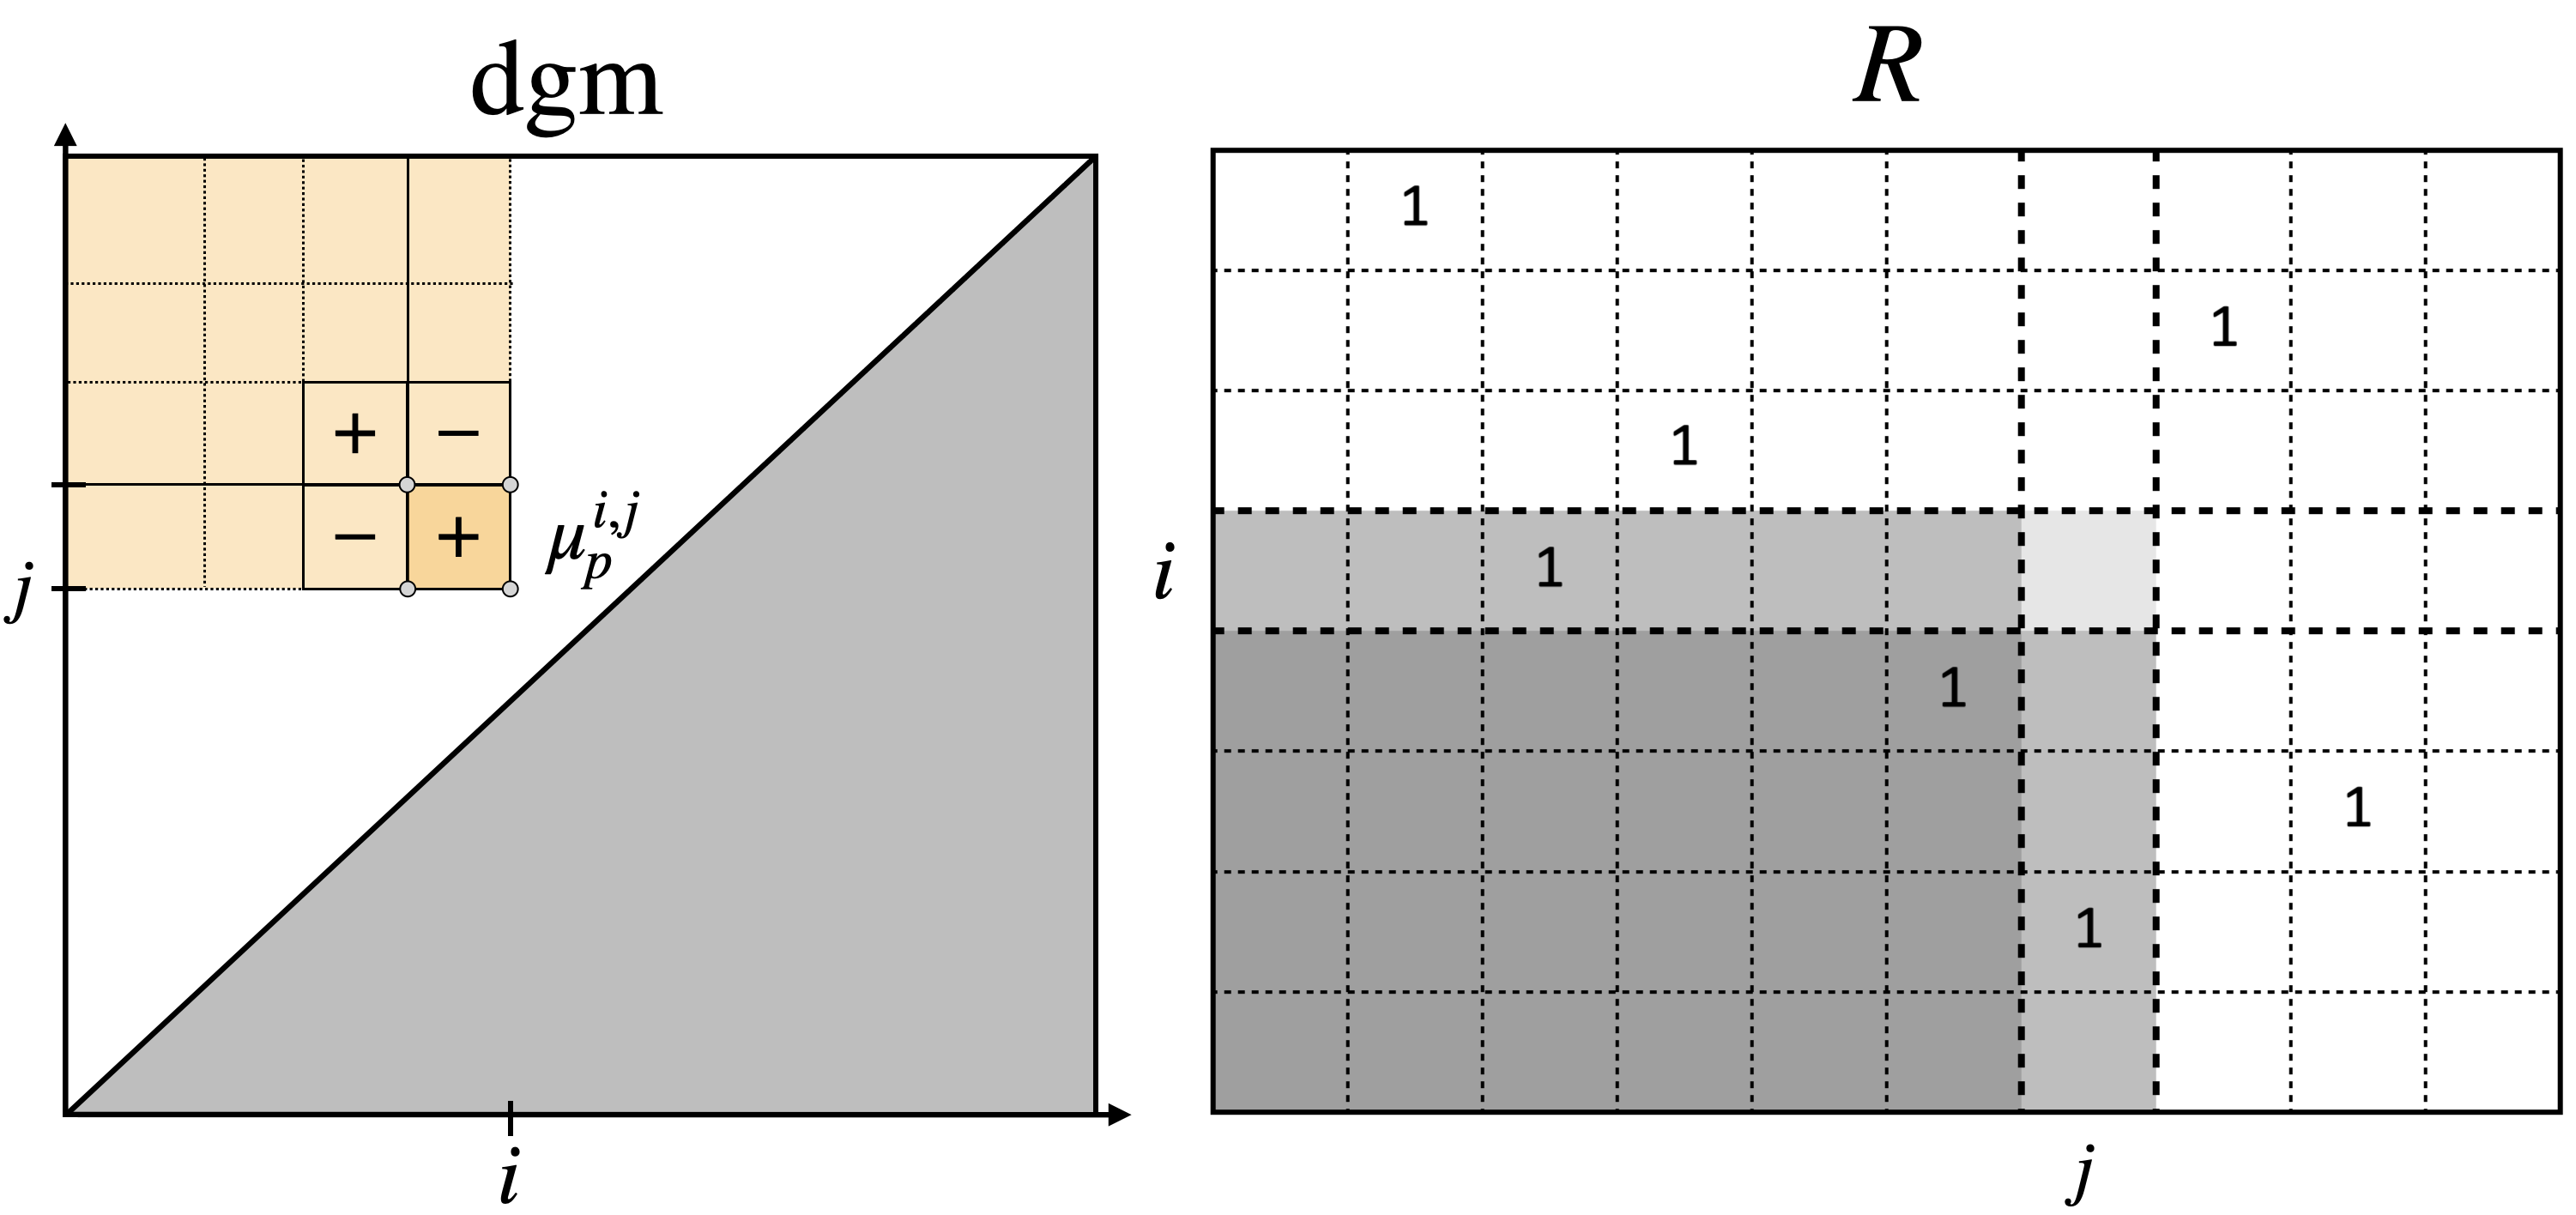
\includegraphics[width=0.45\textwidth]{mult_both}
	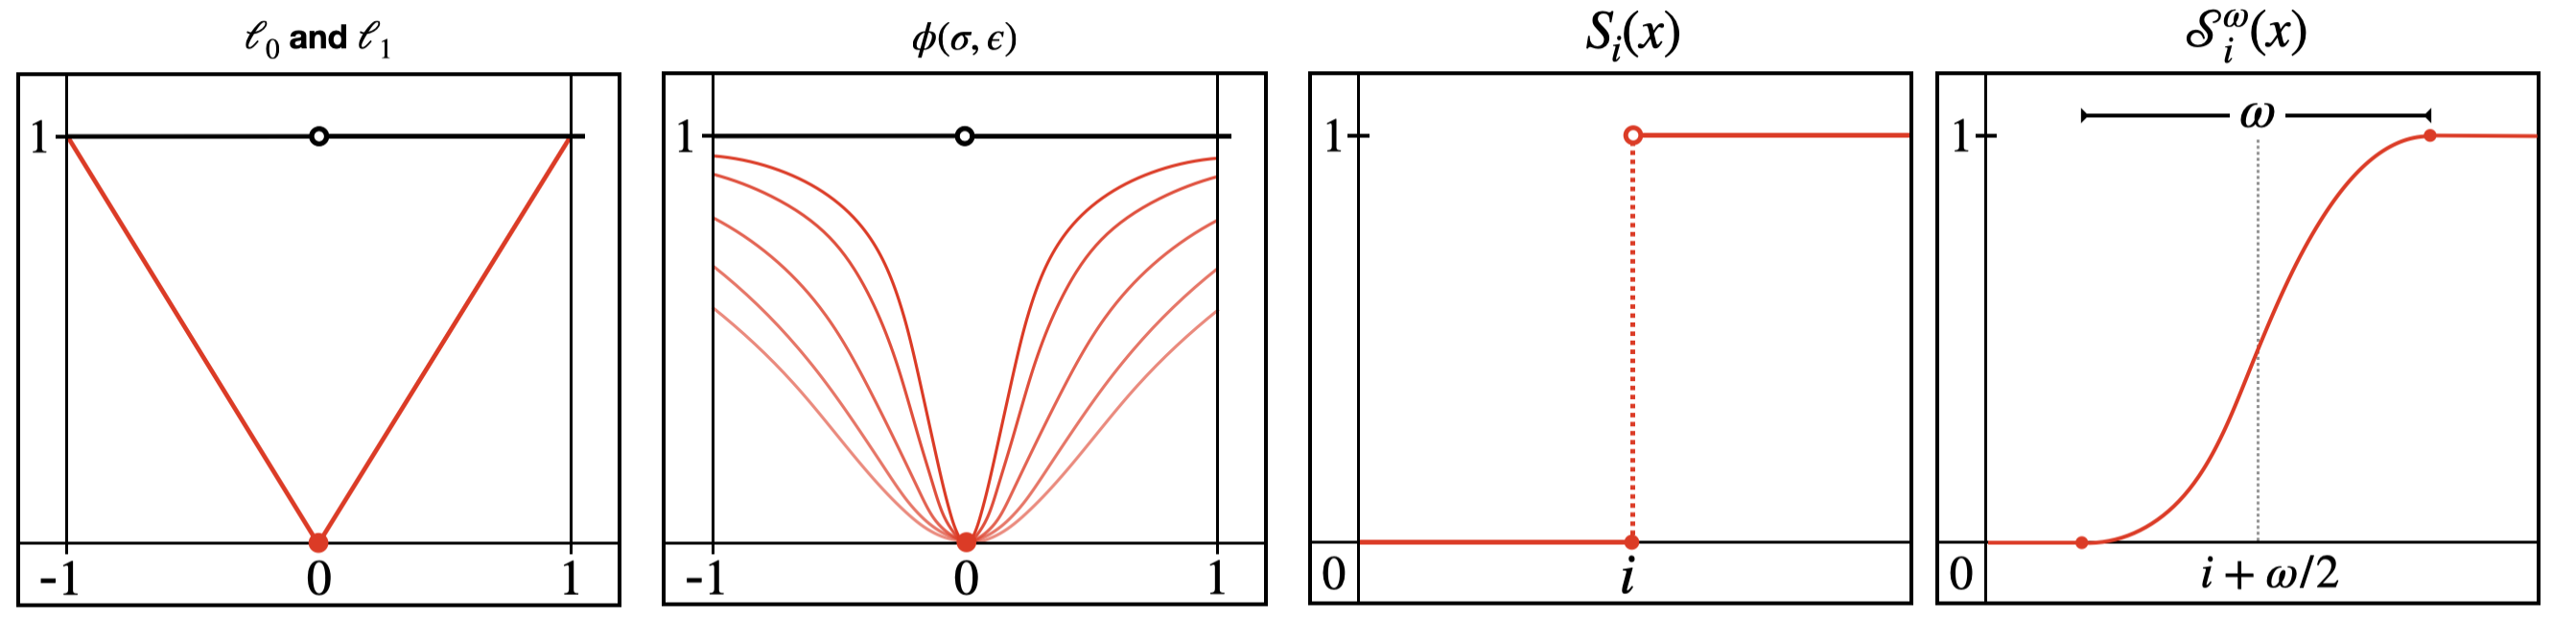
\includegraphics[width=0.90\textwidth]{cont_relax}
	\caption{From left to right---the $\ell_1$ norm (red) forms a convex envelope over the $\ell_0$ (black) pseudo-norm on the interval $[-1, 1]$; 
	$\phi(\cdot, \tau)$ from~\eqref{eq:tikhonov_sf} at various values of $\tau > 0$ (red) and at $\tau = 0$ (black); 
	the step function $S_i(x)$ from~\eqref{eq:rank_equiv_param}; 
	the smoothstep relaxation $\mathcal{S}_i^{\omega}$ from~\eqref{eq:smoothstep}.
	}
	\label{fig:smoothstep}
\end{figure}
%Since smoothstep functions retain the sign of their input, composing with~\eqref{eq:mu_four} and substituting $\mathrm{rank}(\cdot)$ with $\Phi(\cdot, \epsilon)$ yields a continuously-varying $\epsilon$-approximation of the rank function, which we call a \emph{spectral rank function}. 
%\begin{definition}[Spectral Rank]\label{def:smooth_mu}
%Given the same inputs as Proposition~\ref{prop:mu_betti_1},
%let $K$ denote a simplicial complex and parameters $(p, \epsilon, \omega)$ satisfying $p \geq 0$, $\epsilon > 0$, and $\omega > 0$, respectively, define the $\mathcal{A}$-parameterized \emph{spectral persistent Betti number} and \emph{spectral multiplicity} of $R$ as:
%	\begin{equation}\label{eq:bett_cont}
%\hat{\beta}_p^{i,j}(\alpha) = 
%\lVert \Phi_\epsilon^\alpha(\,\hat{I}_{p}^i\,)\rVert_\ast -
%\lVert \Phi_\epsilon^\alpha(\hat{\partial}_{p}^{1, i}) \rVert_\ast - 
%\lVert \Phi_\epsilon^\alpha(\hat{\partial}_{p+1}^{1, j}) \rVert_\ast + 
%\lVert \Phi_\epsilon^\alpha(\hat{\partial}_{p+1}^{i\+\delta, j}) \rVert_\ast \numberthis
%	\end{equation}
%	\begin{equation}\label{eq:mu_cont}
%	\hat{\mu}_{p,\epsilon}^R(\alpha) = 
%		 \lVert \Phi_\epsilon^\alpha(\hat{\partial}_{p\+1}^{j \+ \delta, k}) \rVert_\ast - 
%		 \lVert \Phi_\epsilon^\alpha(\hat{\partial}_{p\+1}^{i \+ \delta, k}) \rVert_\ast -  
%		 \lVert \Phi_\epsilon^\alpha(\hat{\partial}_{p\+1}^{j \+ \delta, l}) \rVert_\ast + 
%		 \lVert \Phi_\epsilon^\alpha(\hat{\partial}_{p\+1}^{i \+ \delta, l}) \rVert_\ast \numberthis
%\end{equation}
%where $\Phi_\epsilon^\alpha(\partial) = (\Phi_\epsilon \circ \partial)(\alpha)$ for any $\alpha \in \mathcal{A}$, $\hat{I}_{p}^i = \mathrm{diag}(\{ \mathcal{S}_i^\omega(f(\tau_j)) \}_{j=1}^{n} )$, and $\hat{\partial}_p$ is $\mathcal{A}$-parameterized $p$-th boundary matrix from~\eqref{eq:rank_equiv_param} with step functions $S_\ast$ replaced by the smoothstep $\mathcal{S}_\ast^\omega$ from~\eqref{eq:smoothstep}.
%\end{definition}
\noindent Noting property (4), since the sum Lipshitz functions is also Lipshitz, it is easy to verify that 
%combining the smoothness of $\mathcal{S}_\ast^\omega$ with the global Lipshitz continuity of~\eqref{def:lowner} that 
replacing the rank function in all of the constitutive terms from Proposition~\ref{prop:mu_betti_1} yields Lipshitz continuous functions whenever the filter function $f_\alpha$ is itself Lipshitz and the step functions from~\eqref{eq:rank_equiv_param} are smoothed ($\omega > 0$). 
\begin{remark} 
	Though $\Phi_\tau$ is a continuously differentiable operator\footnote{In fact, it may be shown to be twice continuously differentiable at $X$ if $\phi$ is twice-differentiable at each $\sigma_i(X)$, see~\cite{ding2018spectral})} in $\mathbb{R}^{n \times m}$ for any $\tau > 0$, % for all $i = 1, \dots, n$, 
	%% TODO: mention that directional differentiability is not enough
	%% see: https://math.stackexchange.com/questions/1410308/is-the-total-differential-the-same-as-the-directional-derivative
its Schatten-1 norm $\lVert\Phi_\tau(X)\rVert_\ast$ is only directionally differentiable everywhere on $\mathbb{R}^{n \times m}$ in the Hadamard sense, due to Proposition 2.2(d-e)  of~\cite{bi2013approximation}. $\lVert\Phi_\tau(X)\rVert_\ast$ is differentiable on the positive semi-definite cone $\mathbb{S}^n_+$.
%We defer the formal definition this persistence-based relaxation and its properties to section~\ref{sec:spri_properties}.
\end{remark}
\noindent
\textbf{Interpretation \#1:} In many applications, it is common to regularize an ill-posed objective function to encourage simpler solutions or to prevent overfitting. 
For example, the classical least-squares approach to solving the linear system $A x = b$ is often augmented with the \emph{Tikhonov regularization} (TR) for some $\tau > 0$:
 \begin{equation}\label{eq:tikhonov}
	x_\tau^\ast = \argmin\limits_{x \in \mathbb{R}^n} \lVert Ax - b\rVert^2 + \tau \lVert x \rVert^2 = (A^T A + \tau I)^{-1} A^T b
\end{equation}
When $\tau = 0$, one recovers the standard $\ell_2$ minimization, whereas when $\tau > 0$ solutions $x_\tau^\ast$ with small norm are favored. 
%\begin{equation}\label{eq:least_squares}
%	x^\ast = \argmin\limits_{x \in \mathbb{R}^n} \lVert A x - b \rVert^2	
%\end{equation}
% ng $A = X$, solutions $x_\epsilon^\ast$ to TR problems in standard form satisfy 
%The solution to~\eqref{eq:tikhonov} is given by the regularized form of the pseudo-inverse given below:  
%\begin{equation}\label{eq:tikhonov_soln}
%	x_\epsilon^\ast = (A^T A + \epsilon I)^{-1} A^T b
%\end{equation}
%To illustrate the relevance of TR with our proposed approximation, 
Similarly, by parameterizing
%\footnote{Similar regularization interpretations may be derived for other choices of $\nu(\epsilon)$ and $p(x)$.}
$\phi$ by $\nu(\tau) = \sqrt{\tau}$ and $p(x) = 2x (x^2 + 1)^{-2}$, one obtains via ~\eqref{eq:phi}:
\begin{equation}\label{eq:tikhonov_sf}
	\phi(x, \tau) = \int\limits_{0}^z \hat{\delta}(z, \tau) dz = \frac{2}{\tau}\int\limits_{0}^z z \cdot  \big((z/\sqrt{\tau})^2+1\big)^{-2} dz = \frac{x^2}{x^2 + \tau} % \nu(1/\epsilon) \cdot p \big( z \, \nu (1/\epsilon) \big ) 
\end{equation}
By substituting $\mathrm{sgn}_+ \mapsto \phi$ and composing with the singular value function~\eqref{def:lowner}, the corresponding spectral rank approximation reduces\footnote{See Theorem 2 of~\cite{zhao2012approximation} for a proof of the second equality.} to the following \emph{trace} formulation:
\begin{equation}\label{eq:tikhonov_1}
%	\Phi_\epsilon(A) = (A^T A + \epsilon \, I_n)^{-1} A^T A, \quad \quad 
	\lVert \Phi_\tau(A) \rVert_\ast = \sum\limits_{i = 1}^n \frac{\sigma_i(A)^2}{\sigma_i(A)^2 + \tau} = \mathrm{Tr}\left[(A^T A + \tau \, I)^{-1} A^T A \right]
	%\mathrm{Tr}\left[(X^T X + \epsilon \, I_n)^{-1} X^T X \right] 
\end{equation}
%Thus, composing the singular value of $\partial_p$ (or $\partial_p^T$) with the spectral function $\phi$ from~\ref{eq:tikhonov_sf} may be interpreted as regularizing the spectrum of the inverse of the given Laplacian.
The relaxation level $\tau$ may be thought of as a regularization term that preferences smaller singular values: larger values smooth out $\lVert \Phi_\tau(\cdot) \rVert_\ast$ by making the pseudo-inverse less sensitive to perturbations, whereas smaller values lead to a more faithful\footnote{This can be seen directly by~\eqref{eq:tikhonov} as well, wherein increasing $\tau$ lowers the condition number of $A^T A + \tau I$ monotonically, signaling a tradeoff in stability at the expense of accuracy.} approximations of the rank.
%$\lVert \Phi_\epsilon(\cdot) \rVert_\ast$ is equivalent to $n$ TR-regularized least-squares problems of the form~\eqref{eq:tikhonov} where $A$ is substituted with $\partial_p$ (or $\partial_p^T$) and $b$ is substituted with an $\alpha$-parameterized $p$-(co)chain.
In this sense, we interpret the quantities obtained by applying~\eqref{def:lowner} to the terms from Proposition~\ref{prop:mu_betti_1} as \emph{regularized RI approximation}.
\\
\\
\noindent \textbf{Interpretation \#2:} 
%In shape analysis applications, diffusion processes are often simulated on meshes or graphs embedded in $\mathbb{R}^d$ to obtain information of about their geometry. 
In shape analysis applications, matrix functions are often used to simulate diffusion processes on meshes or graphs embedded in $\mathbb{R}^d$ to obtain information of about their geometry. 
For example, consider a weighted graph $G = (V, E)$ with $n = \lvert V \rvert$ vertices with graph Laplacian $L_G = \partial_1 \partial_1^T$. 
The \emph{heat} of every vertex $v(t) \in \mathbb{R}^n$ as a function of time $t \geq 0$ is governed by $L_G$ and the \emph{heat equation}~\cite{}: 
\begin{equation}\label{eq:heat_eq}
	v'(t) = -L_G v(0) \quad \Longleftrightarrow \quad L_G \cdot u(x, t) = - \partial u(x, t) / \partial t
\end{equation}
To simulate a diffusion process on $G$ from an initial distribution of heat $v(0) \in \mathbb{R}^n$, it suffices to construct the \emph{heat kernel} $H_t \triangleq \mathrm{exp}(-t \cdot L_G)$ via the spectral decomposition $L_G = U \Lambda U^T$ of $L_G$: 
%where $v(t) \in \mathbb{R}^n$ represents the time-varying vector whose value $v_i(t) \in \mathbb{R}$ represents the amount of heat at vertex $v_i$ at time $t \geq 0$.
%To simulate heat diffusion, given an initial distribution of heat $v(0)$, one begins with a graph $G = (V, E, W)$ with $n = \lvert V\rvert$ vertices and edge weights $W \in \mathbb{R}^m$ representing the conductivity across the $m = \lvert E \rvert$ edges; then, the value of the diffusion process on $G$ at time $t$ is given by \emph{exponential diffusion kernel}:
\begin{equation}\label{eq:heat_kernel}
v(t) = H_t \, v(0), \text{ where } H_t = \sum\limits_{i=1}^n e^{-t \lambda_i} \, u_i \, u_i^T
\end{equation}
The heat kernel is invariant under isometric deformations, stable under perturbations, and is known to contain multiscale geometric information due to its close connection to geodesics~\cite{}. As is clear from~\eqref{eq:heat_kernel}, it is also a matrix function. Now, consider~\eqref{eq:phi} with $\nu(\tau) = \tau$ and $p(\lambda) = \mathrm{exp}(-\lambda_+)$ where $x_+ = \max(x, 0)$: 
\begin{equation}\label{eq:heat_sf}
	\phi(\lambda, \tau) = \int\limits_{0}^z \hat{\delta}(z, \tau) dz = \frac{1}{\tau}\int\limits_{0}^z \mathrm{exp}(-z / \tau) dz = 1 - \mathrm{exp}(- \lambda / \tau), \quad \text{ for all } \lambda \geq 0% \nu(1/\epsilon) \cdot p \big( z \, \nu (1/\epsilon) \big ) 
\end{equation}
In the context of diffusion, observe the parameter $\tau$ is inversely related diffusion time (i.e. $t = 1 / \tau$) and that as $t \to 0$ (or $\tau \to \infty$) the expression $1 - \mathrm{exp}(-\lambda / \tau)$ approaches the $\mathrm{sgn}_+$ function on the interval $[0, \infty)$. 
As above, substituting $\phi$ appropriately into Definition~\eqref{def:lowner} again yields an equivalent trace expression:
%$L_G$: 
\begin{equation}\label{eq:heat_trace}
%	\Phi_\epsilon(A) = (A^T A + \epsilon \, I_n)^{-1} A^T A, \quad \quad 
	\lVert \Phi_\tau(L_G) \rVert_\ast = \sum\limits_{i = 1}^n 1 - \mathrm{exp}(-\lambda_i/\tau) = n - \mathrm{Tr}\left[H_{1/\tau}\right]
\end{equation}
The heat kernel $H_t$ has been shown to fully characterize shapes up to isometry, motivating the creation of various geometric signatures, such as the Heat Kernel Signature (HKS)~\cite{} and the Heat Kernel Trace~\cite{}. 
In this sense, we interpret a spectral rank relaxation using~\eqref{eq:heat_sf} as a \emph{geometrically informative RI approximation}.

% Indeed, informative multiscale signatures, such as the Heat Kernel Signature (HKS), are often used in shape analysis applications due to their rich information content. 
  
%where the matrix function $\mathrm{exp}(-t \cdot \partial_1 \partial_1^T)$, which is the solution the heat equation~\cite{}, is called the \emph{heat kernel} $H_t$ at time $t$:
%$$H_t \triangleq \mathrm{exp}\left(-t \cdot \partial_1 \partial_1^T\right) = U \mathrm{exp}(-t \Lambda) U' = \sum\limits_{i=1}^n e^{-t \lambda_i} \, u_i \, u_i^T$$
%Heat tends to diffuse slower at points with positive curvature and faster at points with negative curvature. 
 
%a function $v(t) \in \mathbb{R}^n$ representing the time-varying vector whose value $v_i(t) \in \mathbb{R}$ represents the value of the diffusion at vertex $v_i \in V$ in a graph $G = (V, E)$ with $n = \lvert V\rvert$ vertices, then the diffusion 
 
%We now discuss the various properties that these smoothed-counting invariants obey. 
%\subsubsection*{Properties}
%
%Basic properties of $\hat{\mu}$. % pseudo-monotonicity, additivity 
%Consider a filtration $(K, f)$ indexed over the real line $f : K \to \mathbb{R}$ whose filter function $f$ is perturbed by some positive amount $\delta > 0$, such that $f' = f + \delta$.
%\begin{equation}
%	\lVert f - f' \rVert_{\infty} \leq \delta 
%\end{equation} 
%Moreover, since operator norm determines the Lipshitz constant of a given function, $\epsilon$ not only plays the role of an accuracy parameter, but as a \emph{smoothing parameter}. 
%Moreover, by the cyclic property of the trace operator, since $X = \partial_1$ here and $L = \partial_1 \partial_1^T = [l_1, l_2, \dots, l_n]$ we have: 
%\begin{equation*}
%	\lVert \Phi_\epsilon(X) \rVert_\ast = \mathrm{Tr}[(L + \epsilon I_n)^{-1} L] = \sum\limits_{i=1}^n (L_\epsilon^{-1} l_i)_i
%\end{equation*}


% ---- PROPERTIES -----
% \subsection{Properties \& Interpretations}\label{sec:spri_properties}
% 
%\subsubsection*{Basic Properties}
% Laplacian Energy
%We start with some basic properties of the function constitutive terms used in both $\beta_p$ and $\mu_p$, which mirror the well-studied Laplacian ``energy'' family of invariants~\cite{}. 
%For some fixed simplicial complex $K$, weight function $w: K \to \mathbb{R}_+$, and index $(i,j) \in \Delta_+$, consider the function:
%$$ \lVert \Phi(\hat{\partial}_p^{i,j} \circ \hat{\partial}_p^{i,j}) \rVert_\ast : \Delta_+ \to \mathbb{R}$$
%where we use the notation $\mathcal{L}_p^{i,j}$ to indicate...
%We have, as its very basic properties: 
%\begin{enumerate}
%	\item $\lVert \Phi(\mathcal{L}_p^{\ast})(K) \rVert_\ast \geq 0$, with equality when $i = j$.
%	%$K^p_i \cap K^{(p+1)}_j = \emptyset$
%	\item If $K$ is the union of disjoint subcomplexes $K_1, K_2, \dots, K_c$, then $\lVert L_p^\ast(K)\rVert_{\Phi} = \sum\limits_{i=1}^c \lVert L_p^\ast(K_i)\rVert_{\Phi}$ 
%	\item If $\tau \in K^p$ does not have a proper coface $\sigma \in K^{p+1}$, then $\lVert L_p^{\text{up}}(K \setminus \tau)\rVert_{\Phi} =\lVert L_p^{\text{up}}(K)\rVert_{\Phi}$. %Similarly, 
%\end{enumerate}
%Many of these properties inherit from the fact that $\lVert \cdot \rVert_\Phi$ is a norm. 
To better understand the implications of the relaxations discussed so far, we establish some of its properties. 
%Let $\mathcal{R} \subset \Delta_+$ denote an arbitrary rectilinear shape with corner points $\partial \mathcal{R} = \{ \, (i_1, j_1), (i_2, j_2), \dots,  (i_h, j_h) \, \}$, 
In what follows, let $\mathcal{L}_p : C^p(K, \mathbb{R}) \to C^p(K, \mathbb{R})$ denote some choice of Laplacian operator and $(\Phi, \phi)$ a $\tau$-parameterized spectral pair satisfying the conditions in definition~\ref{def:lowner}. 
%In full generality, any spectral relaxation generalizing~\eqref{eq:mu_four} will have the form:
%and $R = [i,j] \times [k,l] \subset \Delta_+$. 
%$$ \hat{\mu}^\mathcal{R}_p(\alpha) = \sum\limits_{(i,j) \in \partial \mathcal{R}} s_{ij} \cdot \lVert \Phi(\hat{\mathcal{L}}^{i,j}_p)(\alpha) \rVert_\ast$$
%where the sign $s_{ij} \in \{-1, 1\}$ is determined by the inclusion-exclusion relationship given below.
%Proposition~\ref{prop:include_exclude}
\begin{proposition}\label{prop:include_exclude}
Given any pair $(K, f)$, a rectangle $R = [a,b] \times [c,d] \subset \Delta_+$, and any $\tau$-parameterized spectral function $\phi: \mathbb{R} \to \mathbb{R}$ from definition~\ref{def:lowner}, the spectral rank invariants $\hat{\mu}_{p}^R(\tau)$ and $\hat{\beta}_{p}^{a,b}(\tau)$ satisfy: 
$$ \lim_{\tau \to 0^+ }\hat{\mu}_{p}^R(\tau) = \mu_p^R(K,f), \quad \quad \lim_{\tau \to 0^+ } \hat{\beta}_{p}^{a,b}(\tau) = \beta_{p}^{a,b}(K,f)$$
Moreover, for any $\tau \geq 0$, the following inclusion-exclusion relationship always holds:
$$\hat{\mu}_{p}^R(\tau)= \hat{\beta}_{p}^{b,c}(\tau) - \hat{\beta}_{p}^{a,c}(\tau) - \hat{\beta}_{p}^{b,d}(\tau) + \hat{\beta}_{p}^{a,d}(\tau)$$
\end{proposition}
\begin{proof}
	For limit, use monotonicity + corollary that shows $\phi \to \mathrm{sgn}_+$ in the limit. 
	For the inclusion exclusion, use additivity/ cancellation property / maybe norm properties of $\Phi$ from Chazal. 
\end{proof}
\noindent As an immediate corollary of this, we may generalize the multiplicity function $\hat{\mu}_p^\ast$ to any arbitrary rectilinear $\mathcal{R} \subset \Delta_+$. This follows from the general theory developed by Chazal et al.~\cite{chazal2016structure} on \emph{persistence measures}.
\begin{corollary}
	The spectral-relaxed \emph{persistence measure} of any simple and connected rectilinear sieve $\mathcal{R} \subset \Delta_+$ with $h$ corner points $\partial \mathcal{R} = \{ \, (a_1, b_1), (a_2, b_2), \dots,  (a_h, b_h) \, \}$ given by: 
	$$ \hat{\mu}^\mathcal{R}_p = \sum\limits_{(a,b) \in \partial \mathcal{R}} s_{ab} \cdot \lVert \Phi(\hat{\mathcal{L}}^{a,b}_p) \rVert_\ast$$
	can be computed using at most $O(h)$ spectral rank computations, where the sign $s_{ij} \in \{-1, 1\}$ is determined by the inclusion-exclusion relationship given by Proposition~\ref{prop:include_exclude}. 
\end{corollary}
\begin{proof}
	By the additivity of the multiplicity function, we can vertically or horizontally partition any rectangular into two disjoint rectangles and add their total multiplicity to recover the multiplicity of the whole~\cite{}. Moreover, if $\mathcal{R}$ is simple and hole-free with $h$ corner points, then it is known that it can be decomposed into a minimal set of $h/2-g-1 \sim O(h)$ disjoint rectangles (of which several algorithms are known), where $g$ is the number of axis-parallel line segments connecting concave vertices of $\mathcal{R}$~\cite{}.
\end{proof}

\noindent Though the inclusion-exclusion relationship between the relaxations $\hat{\mu}_{p}^\ast(\tau)$ and $\hat{\beta}_{p}^{\ast}(\tau)$ holds for any $\tau \geq 0$, certain monotonicity properties of $\hat{\beta}_{p}^{\ast}(\tau)$ lose their exactness when $\tau > 0$.
As the rank invariant is fundamentally a combinatorial invariant, this is in some sense necessary.
  
Fortunately, we may bound the degree to $\hat{\beta}_p^\ast$ remains ``Betti-like'' in the sense of being cumulative. 
\begin{proposition}[$\phi$-monotone]
For all $a < b$ and all $c < d$, there exists a positive constant $c_\phi(\tau) \in \mathbb{R}_+$ such that $\hat{\beta}_p^\ast$ satisfies the following monotonicity properties:
%\begin{align*}
%(\tau = 0) & \quad \hat{\beta}_p^{i,k} \leq \hat{\beta}_p^{j,k}, \quad \quad \hat{\beta}_p^{i,k} \geq \hat{\beta}_p^{i,l} \\
%(\tau > 0) & \quad 
\begin{equation}
	\hat{\beta}_p^{a,c} \leq \hat{\beta}_p^{b,c} + c_\phi(\lvert a - b \rvert), \quad \quad \hat{\beta}_p^{a,c} \geq \hat{\beta}_p^{a,d} - c_\phi(\lvert c - d \rvert)
\end{equation}
When $\phi = \mathrm{sgn}_+$, $c_\phi$ is identically zero, recovering the monotonicity of the PBN (see section 2.1 of~\cite{cerri2013betti}). 
%the constant map $c_\phi(x) = 0$
%\end{align*}
\end{proposition}
\begin{proof}
	Use Proposition above part (b) with a specific $\phi$, then use PBN property.
\end{proof}
In fact, under mild conditions, its been shown that the Tikhonov relaxation $\phi_\tau$ is actually a \emph{uniform} approximation of the rank function~\cite{}. 
%This is important in rank minimization contexts, wherein it is 


%\begin{corollary}
%	For every $\alpha \in \mathcal{A}$, there exists a value $\tau^\ast > 0$ such that $\lfloor$
%\end{corollary}



%TODO: 
%\noindent
%As signaled in the outline of the paper, one tradeoff in relaxing the exact monotonicity of the $\beta_p$ is \emph{relative} stability in the associated invariants as function of $\alpha \in \mathcal{A}$. 
%\begin{proposition}[Relative stability]
%Let $\alpha, \alpha' \in \mathbb{R}$ denote parameters satisfying $\lvert \alpha - \alpha' \rvert \leq \delta$, $\mathcal{R} \subset \Delta_+$ a fixed sieve, and let $\hat{\mu}_p(\alpha')$ represent a \emph{relative perturbation} of $\hat{\mu}_p(\alpha')$
%%each of the constitutive terms of ~\eqref{} satisfy $\hat{\mathcal{L}}^\ast_p(\alpha') = Q^T \hat{\mathcal{L}}^\ast_p(\alpha) Q$ 
%$$ 
%\hat{\mu}_p^\mathcal{R}(\tilde{\alpha}) = \sum\limits_{(i,j) \in \partial \mathcal{R}} s_{ij} \cdot \lVert Q_{i,j}^T \left ( \Phi(\hat{\mathcal{L}}^{i,j}_p)(\alpha) \right ) Q_{i,j} \rVert_\ast
%$$
%where $Q \in \mathbb{R}^{n \times n}$ is symmetric and non-singular. Then the spectral multiplicities $\hat{\mu}_p^R(\alpha)$ and $\hat{\mu}_p^R(\alpha')$ satisfy: 
%$$\lvert \, \hat{\mu}_p^\mathcal{R}(\alpha') - \hat{\mu}_p^\mathcal{R}(\alpha) \, \rvert \leq \sum\limits_{(i,j) \in \partial\mathcal{R}} \lVert I - Q_{i,j}^T Q_{i,j}\rVert_2 $$
%\end{proposition}

%the  we have: $Q^T A Q $where $Q \in \mathbb{R}^{n \times n}$ is non-singular and $A, \tilde{A} \in \mathbb{R}^{n \times n}$ are the original and perturbed matrices, respectively. 
%%If the perturbation is small, the intuition is that $Q^T Q$ will be close to identity. This is captured by an extension of Ostrowski's Theorem, as summarized by Li~\cite{}. 

%\begin{proof}
%	Li et al established $\lvert \tilde{\lambda}_j - \lambda_j \rvert \leq \lambda_j  \cdot  \lVert I - Q^T Q\rVert_2 \quad \Leftrightarrow \quad\tilde{\lambda_j} = \lambda_j(1 + \delta_j), \quad \lvert \delta_j \rvert \leq \lVert I - Q^T Q\rVert_2 $
%\end{proof}

%\begin{proposition}\label{prop:include_exclude}
%For any $\tau > 0$ and spectral function $\phi : \mathbb{R} \to \mathbb{R}$ satisfying~\eqref{eq:phi}, the spectral multiplicity invariant $\hat{\mu}_{p,\tau}^R$ of any rectangle $R = [i,j] \times [k,l] \subset \Delta_+$ obeys the following inclusion exclusion: 
%$$ \hat{\mu}_{p,\tau}^R(K, f)= \hat{\beta}_{p,\tau}^{j,k} - \hat{\beta}_{p,\tau}^{i,k} - \hat{\beta}_{p,\tau}^{j,l} + \hat{\beta}_{p,\tau}^{i,l}
%$$
%\end{proposition}
%\begin{proof}
%	Use additivity / inclusion exclusion / cancellation property / maybe norm properties of $\Phi$
%\end{proof}
%$$ \hat{\mu}_p^{\mathcal{R}}(K,f) = \mathrm{card}\left(\restr{\mathrm{dgm}_p(K,f)}{\mathcal{R}} \right) $$ 



%any simple and connected rectilinear sieve $\mathcal{R} \subset \Delta_+$ with $h$ corner points 
%Another property is 



%\subsubsection*{Stability}
%One disadvantage of rank functions restricted to subsets of the real-plane is that they are integer-valued and unstable. Indeed, one may easily construct examples of $\mathcal{A}$-parameterized filtrations 
%$(K, f_\alpha)$ where $\lVert \mu_p^R(\alpha) - \mu_{p}^R(\alpha + \delta) \rVert \sim O(\lvert K_p \rvert )$ for some arbitrarily small $\delta > 0$, as there may be up to $O( \lvert K_p \rvert)$ points in $\mathrm{dgm}_p(K)$.
%On the other hand, our spectral rank invariants derive from symmetric Laplacian operators, and the spectra of these are known to stable under certain kinds of perturbations~\cite{bhatia2013matrix}. 
%% is a well-studied topic in numerical analysis~\cite{bhatia2013matrix}, which should inherit  
%%Intuitively, since both counting invariants are $0$ outside of the portions of $\Delta_+$ they restrict  too, it's always possible to encounter situations where small changes in the input affect the corresponding invariant in a non-Lipshitz way. 
%%Relaxing $\mu_p^R \mapsto \hat{\mu}_p^R$ fixes this instability when $\epsilon > 0$, though the Lipshitz constant may be arbitrarily high.
%In what follows, we investigate how to exploit the structure of $L_p^\ast$ and the smoothness of $f_\alpha$ to stabilize the constitutive terms in $\hat{\mu}_p^\ast$ and $\hat{\beta}_p^{\ast}$. 
%We will exclusively consider the spectra of normalized combinatorial Laplacian operators:
%$$ \lVert \Phi( \partial_p 	) \rVert_\ast = \sum\limits_{i = 1}^n \phi_{\epsilon}(\lambda_i(\mathcal{L}))
%$$
%under some choice of regularization $(\Phi, \phi)$ and $\epsilon > 0$. Our focus is on the \emph{relative} perturbation model, which seeks to describe perturbations of the form: 
%$$ \tilde{A} = Q^T A Q $$
%where $Q \in \mathbb{R}^{n \times n}$ is non-singular and $A, \tilde{A} \in \mathbb{R}^{n \times n}$ are the original and perturbed matrices, respectively. If the perturbation is small, the intuition is that $Q^T Q$ will be close to identity. This is captured by an extension of Ostrowski's Theorem, as summarized by Li~\cite{}. 
% $$ \lvert \tilde{\lambda}_j - \lambda_j \rvert \leq \lambda_j  \cdot  \lVert I - Q^T Q\rVert_2 \quad \Leftrightarrow \quad\tilde{\lambda_j} = \lambda_j(1 + \delta_j), \quad \lvert \delta_j \rvert \leq \lVert I - Q^T Q\rVert_2 $$ 
% Connections to Laplacian Energy


 
 
\section{Computational Implications}\label{sec:computational_imp}
%\subsection*{An quadratic-time rank computation}
%In this section, we discuss several of the computational advantages that arise by combining the results of section~\ref{sec:spectral_sec}, focusing on iterative subspace acceleration techniques that decouple explicit matrix representations from the computation.

%As the singular values of boundary operators can be obtained are the square roots of eigenvalues of an appropriate Laplacian operator, we focus on spectral methods specialized for symmetric positive semi-definite operators.
%In the following sections, we (1) recall the method of minimized iterations in section~\ref{sec:lanczos_it}, (2) explore the efficiencies and subtleties of simplicial Laplacian $\mathtt{matvec}$ operators, and (3) discuss the modern advances to estimating spectral quantities of combinatorial Laplacians efficiently, such as preconditioning methods and convergence rates. 

%In particular, combinatorial Laplacians form a subset of the very important class of diagonally dominant (DD) matrices. % combinatorial number system


% Benefits of rank(A) = < non-zero eigenvalues >
\subsection{Exact computation}\label{sec:lanczos_it}
As evidenced by Section~\ref{sec:spectral_sec},
%sections~\ref{sec:laplacian_theory2} and~\ref{sec:spectral_relax}, 
computing $\hat{\mu}_p^\ast$ and $\hat{\beta}_p^\ast$ may be reduced to computing eigenvalues of $p$-Laplacians. To do this efficiently, we employ the \emph{Lanczos method}~\cite{lanczos1950iteration}, which estimates the eigenvalues of any symmetric linear operator $A$ via projection onto successive Krylov subspaces. 
Formally, given a symmetric $A \in \mathbb{R}^{n \times n}$ with eigenvalues $\lambda_1 \geq \lambda_2 > \dots \geq \lambda_r > 0$ and a vector $v \neq 0$, the Lanczos method generates the triplet:
%the order-$j$ Krylov subspaces of the pair $(A, v)$ are the spaces spanned by: 
%\begin{equation}
%	\mathcal{K}_j(A, v) \triangleq \mathrm{span}\{ A^0 v, A^1 v, A^2 v, \dots, A^{j-1}v \}	
%\end{equation}
\begin{align*}
K &= [\, A^0 v \mid A^1 v \mid A^2 v \mid \dots \mid A^{r-1}v \,]  \\
Q &= [\, q_1, q_2, \dots, q_r \,] \gets \mathrm{qr}(K)   \\
T &= Q^T A Q 
\end{align*}
where $K \in \mathbb{R}^{n \times r}$ is the \emph{Krylov matrix} with respect to $(A, v)$, $Q \in \mathbb{R}^{n \times r}$ is an orthogonal change-of-basis, and $T \in \mathbb{R}^{r \times r}$ is symmetric tridiagonal \emph{Jacobi matrix}. 
It is well known that $Q$ is a similarity transform, i.e. $T$ preserves the spectrum of $A$ and the problem of finding eigenvalues reduces to diagonalizing $T$.

The Lanczos method is often called a ``matrix free'' method due to the fact that only a matrix-vector product operator $v \mapsto Av$ is required for execution---$A$ need not necessarily be stored in memory explicitly.  
This aspect alone suggests Lanczos may be a viable low-memory option for computing eigenvalues. 
%keeps its memory footprint small, as the storage complexity of effectively reduces to that of $A$.
%For this reason, the Lanczos method is often preferred for sparse or heavily structured operators
Indeed, due to its \emph{three-term recurrence}~\cite{simon1984analysis}, the Lanczos method requires just three $O(n)$-sized vectors and a few $O(n)$ vector operations to obtain $T$---neither $K$ nor $Q$ need be formed explicitly. 
\begin{lemma}[\cite{parlett1994we}]\label{lemma:exact_arith_lanczos}
	Given a symmetric rank-$r$ matrix $A \in \mathbb{R}^{n \times n}$ whose matrix-vector operator $x \mapsto A x$ requires $O(\eta)$ time and $O(\nu)$ space, the Lanczos iteration computes $\Lambda(A) = \{ \lambda_1, \lambda_2, \dots, \lambda_r \}$ in $O(\max\{\eta, n\}\cdot r)$ time and $O(\max\{\nu, n\})$ space, when computation is done in exact arithmetic. 
\end{lemma}
%\begin{corollary}\label{cor:finite_arith_lanczos}
%	Given the same inputs as Lemma~\ref{lemma:exact_arith_lanczos}, any implementation that computes $\Lambda(A) = \{ \lambda_1, \lambda_2, \dots, \lambda_r \}$ using the Lanczos iteration in finite-precision arithmetic requires $\Omega(\max\{\eta, n\} \cdot r)$ time and $\Omega(\max\{\nu, n\})$ space complexity. 
%\end{corollary}
%\subsection{The combinatorial Laplacian \texttt{matvec}}\label{sec:comb_lap}
\noindent As evidenced by Lemma~\ref{lemma:exact_arith_lanczos}, the efficiency of the Lanczos method depends on the availability of a fast \texttt{matvec} operator, such as those arising from structured or sparse\footnote{For example, the Lanczos method has expected time complexity $O(n z r)$ for sparse matrices containing an average of $z$ nonzeros per row~\cite{golub2013matrix}} operators.
%the former of which arises in the decomposition of symmetric matrices while the latter depends on the structure of $A$. 
An exemplary structured operator is the graph Laplacian $L = \partial_1 \partial_1^T$, whose $x \mapsto L x$ operation has complexity linear in the number of edges $\lvert E \rvert$ due to its graph structure.
%In particular, sign cancellations in $\partial_1 \partial_1$ ensures the operation $x \mapsto (D - A)x$ reduces to a two phase computation: one to accumulate the degrees of the vertices and one to subtract off components from neighboring vertices, both of which can be computed in $O(\lvert E \rvert)$ by enumerating edges in e.g. an edgelist data structure.
Though this is result is well established for the graph Laplacian, it is not immediately clear whether a similar guarantee generalizes to combinatorial Laplacian operators derived from simplicial complexes---our next result affirms this.
% and as previously mentioned, the Lanczos iteration is only efficient if one as has access to a fast matrix-vector product.  By our definition of rank in~\eqref{eq:rank_def}, this implies $\mathrm{rank}(\partial) = \mathrm{rank}(\partial \partial^T) = \mathrm{rank}(\partial^T \partial)$ and thus the Lanczos method may be readily applied to $\partial \partial^T$ or $\partial^T \partial$. % up to a change in the multiplicity of the zero 
%since the latter are by definition the nonnegative square roots of former and thus . 
%Since a $p+1$-simplex has $p$ proper faces in its boundary, and we need to iterate through the $p+1$ simplices $\sigma \in K^{p+1}$ just once in the case of the $\mathrm{up}$-Laplacian,
%We combine the above observations into a proposition. 
\begin{lemma}\label{lemma:matvec_lap}
	For any $p \geq 0$ and simplicial complex $K$ with $n = \lvert K^p \rvert$ and $m = \lvert K^{p+1} \rvert$, if there exists a hash function $h: K^p \to [n]$ with $O(1)$ access time and $O(c)$ storage, then there exists a two-phase algorithm for computing the product $x \mapsto L_p x$ in $O(m(p+1))$ time and $O(\mathrm{max}(c,m))$ space. 
	%Moreover, the matrix-vector product may be implemented \emph{efficiently} in the sense that the memory access pattern to $K^{p+1}$ can easily be made cache-optimal. 
	%If $K$ is sufficiently dense such that $m \sim O(\lvert V \rvert^{p+1})$, we may accelerate the computation via~\cite{}. 
\end{lemma}
%\begin{proof}
%	See appendix section~\ref{app:lap_matvec}
%\end{proof}
\noindent The algorithm and proof are given in appendix section~\ref{app:lap_matvec}. From a practical perspective, many hash table implementations achieve expected $O(1)$ access time using only a linear amount of storage, and as $p \geq 0$ is typically quite small---the operation $x \mapsto L x$ in practice exhibits $\approx O(m)$ time and space complexities. 
%This matrix-free approach has the same time complexity as is only a slight improvement over $\partial_p$ 
We delegate more practical issues regarding the computation to appendix~\ref{alg:lap_matvec}.
Combining Lemmas~\ref{lemma:exact_arith_lanczos} and~\ref{lemma:matvec_lap} yields our main result. 
\begin{proposition}\label{prop:spectral_rank_complexity}
For any constant $p \geq 0$ and box $R = [a,b] \times [c,d] \subset \Delta_+$, the persistent multiplicity function $\mu_p^R(K)$ derived from a simplicial complex $K$ with 
$n_{ad} = \lvert K_d^{p} \rvert - \lvert K_a^{p} \rvert$ and $m_{ad} = \lvert K_d^{p+1} \rvert - \lvert K_a^{p+1} \rvert$, can be computed in exact arithmetic in the following time and space complexities:
%$n = \lvert K^p \rvert$ and $m = \lvert K^{p+1} \rvert$ simplices can be computed in: 
$$ \mu_p^R(K) \overset{\mathrm{time}}{=} O(n_{ad}\cdot m_{ad}), \quad \mu_p^{R}(K) \overset{\mathrm{space}}{=} O(\mathrm{max}(n_{ad}, m_{ad}))$$
In particular, when $R = [-\infty, \ast] \times [\ast, +\infty]$, $\mu_p^R(K)$ has time and space complexities of $O(nm)$ and $O(\mathrm{max}(n, m))$, respectively, where $n = \lvert K^{p} \rvert$ and $m = \lvert K^{p+1} \rvert$.
\end{proposition}	
%\subsection{Computing diagrams}\label{sec:pers_alg}
%\begin{remark}
\noindent
It's worth noting that the standard reduction-family of algorithms computes the $p$-th persistent homology of a filtration $K$ of dimension $p + 1$ and of size $N = \lvert K \rvert \sim O(\lvert K^{p+1}\rvert)$ in $O(N^3)$ time and $O(N^2)$ space, respectively---these bounds are actually tight $\Theta(N^3)$.
%\footnote{
%A counter-example is given in the online note by Dmitriy Morozov. "Persistence algorithm takes cubic time in worst case." \url{https://citeseerx.ist.psu.edu/document?repid=rep1&type=pdf&doi=9f5b7f8d6616f6c1713178be0664b2c254960455}).
%}. 
Interestingly, Chen and Kerber~\cite{chen2011output} have shown that since the persistence diagram contains at most $N/2 = O(N)$ points, it may be constructed using at most $2N - 1$ ``$\mu$-queries'' (evaluations of $\mu_p^R$) via a divide-and-conquer scheme on the index-persistence plane. 
Since both $\lvert K^{p}\rvert$ and $\lvert K^{p+1}\rvert$ are trivially bounded above by $O(N)$, by Proposition~\ref{prop:spectral_rank_complexity}, we may recover the same $O(N^3)$ time complexity of the reduction algorithm using only rank computations, and we improve the space complexity by a factor of $N$, though at the cost of not having immediate access to cycle representatives.  
%	In contrast to the reduction algorithm Chen and Kerber's algorithm can detect  
	%In practice, the matrices involved in the computation are much 
%\end{remark}
\begin{remark}
	A similar result for computing [non-persistent] Betti numbers of simplicial complexes over finite fields was given by Edelsbrunner and Parsa in~\cite{}, wherein the complexity of computing the Betti numbers of a 2-dimensional simplicial complex $K$ with $n$ vertices was shown to be $\Omega(r(n,m))$, where $r(n,m)$ is the complexity of computing the rank of an $n$-by-$n$ binary matrix with $m$ non-zero entries. 
%	Though we also reduce a Betti number computation to constant number of rank computations, our result is distinct in that (1) we focus on the exact computation model in $\mathbb{R}$, and (2) we relegate the rank computation to the Lanczos procedure, as opposed to reduction, and finally (3) we address the space complexity. 
\end{remark}

%\begin{proposition}\label{prop:spectral_rank_complexity}
%For any constant $p \geq 0$, the spectra $\Lambda(L_p)$ of a rank-$r$ combinatorial Laplacian operator $L_p: \mathbb{R}^n \to \mathbb{R}^n$ derived from a simplicial complex $K$ with $n = \lvert K^p \rvert$ and $m = \lvert K^{p+1} \rvert$ can be computed in $O(mr)$ time and $O(m)$ storage via the Lanczos iteration, when carried out in exact arithmetic. 
%\end{proposition}	
%There are multiple optimizations we may make in the evaluation of~\eqref{eq:l_up_matvec} over the traditional sparse matrix multiplication---some due to the simplicial structure of the underlying operator, and some due to the permutation invariance mentioned in the previous section. 
%\begin{corollary}
%	For any constant $p \geq 0$, the persistent rank-based quantities $\mu_p^\ast(K)$ and $\beta_p^\ast(K)$ derived from a simplicial complex $K$ with $n = \lvert K^p \rvert$ and $m = \lvert K^{p+1} \rvert$ simplices can be computed in $O(mr)$ time and $O(m)$ storage via the Lanczos iteration, when carried out in exact arithmetic. 
%\end{corollary}




%For this reason, practitioners have tended to avoid 

\subsection{Randomized $(\eta, \epsilon)\,$-approximation via trace estimation}\label{sec:iterative_approx}
As in~\cite{parlett1994we}, Proposition~\ref{prop:spectral_rank_complexity} assumes an exact arithmetic computation model to simplify both the presentation of the theory and the corresponding complexity statements. In practice, finite-precision arithmetic introduces \emph{both} rounding and cancellation errors into the computation, which primarily manifests as loss of orthogonality between the Lanczos vectors---among other difficulties, these errors affect both the convergence rate and termination conditions of the algorithm~\cite{parlett1994we}, prohibiting its use practically.
%such as the generation of spurious ``ghost'' eigenvalues
Though many improvements have been proposed (e.g. selective re-orthogonalization, implicit restarting), it is well-known that the Lanczos method is not efficient at obtaining accurate eigenvalue approximations on the interior of the spectrum. 

Fortunately, accurately estimating eigenvalues is not necessary for accurately estimating the rank. Unlike eigenvalue estimation, it has been shown that using Lanczos in finite precision arithmetic is stable for matrix function\footnote{Recall that if $A \in \mathbb{R}^{n \times n}$ has eigenvalue decomposition $A = U \Lambda U^T$, the matrix function $f(A) \in \mathbb{R}^{n \times n}$ is $U f(\Lambda) U^T$, where $f(\Lambda)$ applies $f$ to each diagonal entry of $\Lambda$.} approximation $x \mapsto f(A)x$:
%A common application of the Lanczos method is to approximate the action $x \mapsto f(A)x$, where $f(A) = U f(\Lambda) U^T$ represents a matrix function\footnote{Recall a matrix function...} defined for the pair $(A, f)$:
$$Q^T A Q = T \quad \Leftrightarrow \quad f(A)v \approx \lVert x \rVert \cdot Q f(T) e_1$$
%Substituting $f(\lambda) = \sign_+$, 
%As our spectral RI approximation $\Phi$ derives from matrix functions, 
In particular, Paige's A27 Lanczos variant~\cite{} executed up to degree $k$ is no worse than the best degree-$p$ polynomial approximation to $f$, for any $p < k$.
For general matrix functions, this implies that finite-precision Lanczos essentially matches the strongest known exact arithmetic bounds.  
%In particular, to estimate the rank
The above results underpin the \emph{stochastic Lanczos quadrature} (SLQ) method employed by Ubaru et. al~\cite{ubaru2016fast}, who propose the use of SLQ method for estimating the trace of a matrix function by means of a Girard-Hutchinson (GH) estimator: 
$$ \mathrm{tr}(f(A)) = \sum\limits_{i=1}^{n} e_i^T f(A) e_i  \approx \frac{n}{n_v} \sum\limits_{j=1}^{n_v} e_1^T f(T_m^{(j)}) e_1  = \frac{n}{n_v} \sum\limits_{j=1}^{n_v} \left ( \sum\limits_{i=1}^m \tau_i^{(j)} f(\theta_i^{(j)}) \right ), \quad \tau_{i} = [e_1^T y_i]^2$$ 
where $T_m^{(j)}$ represents the result applying Lanczos to the degree-$(m+1)$ Krylov expansion of $(A, v^{(j)})$ and $(\theta_i, y_i)$ represent the Rayleigh-Ritz pairs associated with the tridiagonal eigendecomposition $T_m = Y \Theta Y^T$. 
When $v^{(j)} \sim \mathcal{D}$ is distributed on a sub-Gaussian distribution satisfying $\mathbb{E}[v^{(j)} \otimes v^{(j)}] = I$, the approximation above is known to be an unbiased estimator of $\mathrm{tr}(f(A))$.
%and $\tau_i = [e_1^T y_i]$ represents the square of the first component of the $i$th Ritz vector $y_i$. 
Note that setting $f(\lambda) = \mathrm{sgn}_+(\lambda)$ yields $\mathrm{tr}(f(A)) = \sum_{i=1}^n\mathrm{sgn}_+(\lambda_i) = \mathrm{rank(A)}$, motivating the use of trace estimation methods  for both rank and spectral sum approximation. 
%Using Lanczos quadrature estimates, the theory above enables the GH estimator to extend to be used as an estimator for the trace of a matrix function:
Under mild assumptions (see~\cite{ubaru2016fast}), and if the function of interest $f: [a,b] \to \mathbb{R}$ is analytic on $[\lambda_{\text{min}}, \lambda_{\text{max}}]$, then for constants $\epsilon, \eta \in (0, 1)$ the output $\Gamma$ of the GH estimator satisfies: 
$$\mathrm{Pr}\Bigg[ \lvert \mathrm{tr}(f(A)) - \Gamma \rvert \leq \epsilon \lvert \mathrm{tr}(f(A)) \rvert \Bigg] \geq 1 - \eta $$
In other words, we can achieve a relative $\epsilon$-approximation of $\mathrm{tr}(f(A))$ with success probability $\eta$ using on the order of $O(\epsilon^{-2} \log(\eta^{-1}))$ evaluations of $e_1^T f(T_m) e_1$, where each $T_m$ is generated by applying degree-$(m+1)$ Lanczos to pairs $(A, v)$ generated over random $v \sim \mathcal{D}$. This probabilistic guarantee is most useful when $\epsilon$ is not too small, i.e. only a relatively coarse approximation of $\mathrm{tr}(f(A))$ is needed.
More recent results by Musco et al.~\cite{} show how this approach can be modified to obtain a $(1 \pm \epsilon)$ approximation using only  $\sim O(\epsilon^{-1} \log(\eta^{-1}))$ samples using deflation techniques, though this does require additional re-orthogonalization and storage costs.


%Note that to estimate the rank  

%\subsection{Empirical experiments}
% The first and most general application of the work presented here is the matrix-free computation of persistent rank invariants in effectively $O(n^2)$ time and $O(m)$ storage, where $n = \lvert K^p \rvert$ and $m = \lvert K^{p+1}\rvert$. 
%Here, the primary difference between the persistent Betti number $\beta_p^{i,j}$ at index $(i,j) \in \Delta_+$ and the multiplicity function $\mu_p^{R}$ on some box $R=[i,j] \times [k,l]$ is that the former can capture essential homology classes (cycles which never die), whereas the multiplicity function by definition can only capture those classes whose persistence is bounded. 
%Our approach to computing persistence diagrams is to simply compute the multiplicities $\mu_p^{i,j}$ of all points $i,j \in \Delta_+$ following the algorithm from Chen \& Kerber~\cite{chen2011output}. The central idea of their approach is to compute the diagram by repeated multiplicity computations (``$\mu$-queries'') on the filtration boundary matrix $\partial$ in a divide-and-conquer like approach.  
%The first and most general application of the work presented here is the matrix-free computation of the spectra of various combinatorial Laplacian operators. 
%Since we may recover both the persistence diagram~\cite{chen2011output} and the rank invariants by repeated spectral computations, we focus examining the time and storage characteristics of Laplacian spectral computation itself rather than its corresponding persistence computations. 
To demonstrate this empirically, we sampled $30$ random graphs according to the Watts-Strogatz~\cite{} rules with parameters $n=500, k=10, p=0.15$. These graphs tend to exhibit `small world' characteristics inherited by many real-world networks, such as social networks, gene networks, and transportation networks.  
For our purposes, since the graph distance between pairs of nodes scale logarithmically with the size of the graph, we ensure the sampled random graphs to be uniformly sparse. 
The corresponding incidence matrix $\partial_1 \in \mathbb{R}^{n \times m}$ and up-Laplacians $L_0^{\mathrm{up}} \in \mathbb{R}^{n \times n}$ would have $\approx 5,000$ and  $\approx 5,500$ non-zero entries, were they to be formed explicitly, which are weighted according randomly by embedding the graph in the plane and filtering  graph via its sublevel sets in a random direction. 
%A much smaller Watts-Strogatz graph of the same type (but with only $50$ nodes) is shown on the left-side of figure~\ref{fig:watts_strogatz}, colored by the filtering of its lower stars. 
\begin{figure}[t]
	\includegraphics[width=\textwidth]{presentations/images/watts_strogatz_perf.png}
	\caption{Random Watts-Strogatz ``Small world'' graph example}
	\label{fig:watts_strogatz}
\end{figure}
To test the scability of the laplacian operator studied here, we computed various percentages of the spectra of these $30$ graphs via iterative methods discussed in section~\ref{} and reported various of their time- and storage- related statistics in figure~\ref{fig:watts_strogatz}. 
All statistics reported are the average statistics collected from all 30 random graphs, which were collected using  various iterative methods implemented the PRIMME software~\cite{}. 
On the far left of figure~\ref{fig:watts_strogatz}, we display a random metric embedding of a small Watts-Strogatz graph to convey the structure of the type of graphs we consider. 
On the left side of figure~\ref{fig:watts_strogatz} next to the example network model, we record the ratio of $\mathtt{matvec}$ operations (relative to $n$) needed to compute $p\%$ of the spectrum as a function of the maximum number basis vectors kept in-memory for reorthogonalization purposes. 
The ideal Lanczos method needs just $3$ such vectors in exact arithmetic due to the three-term recurrence, justifying the space complexity record in~\ref{lemma:exact_arith_lanczos}; in contrast, with finite-precision arithmetic, one needs additional basis vector to ensure the orthonormality of the eigenvectors to machine precision.
Each additional basis vector simultaneously increases both the cost of performing a Lanczos step and the accuracy of the orthogonalization, which subsequently decreases the number of total \texttt{matvec} operations needed. 
As one can see from the plot, having $\approx 20-25$ basis vectors is more than enough to ensure the ratio of $\mathtt{matvec}$ operations is kept to a small constant (in this case, less than $5$) when approximating any portion of the spectra. 
This justifies our claim that combinatorial Laplacian operators, for many real-world data sets, requires just $O(m)$ memory complexity to compute eigenvalues (and thus, the persistent rank invariants).
 The remaining two figures on the right side of figure~\ref{fig:watts_strogatz} show the same ratio of $\mathtt{matvecs}/n$---effectively the constant associated with quadratic time complexity statement in~\ref{lemma:exact_arith_lanczos}


\subsection{Apparent pairs optimization}
%One of the unique features of the reduction algorithm is how many improvements have been made to it compared to the generic PLU decomposition. Nowadays, many adances to the direct method of computing persistence have been made including e.g. the implicit matrix reduction, cohomology, the clearing optimization, the chunking algorithm, and so on. 
%As our approach to computing persistent related quantities does not involve reduction, it is not immediately clear if these optimizations are applicable. 
One of the defining aspects of the computation is that, unlike the reduction algorithm, execution does not require matrix decomposition. 
% it does not decompose the filtered boundary matrix $\partial$. 
While this distinction is important, it does not necessarily bar the transfer of persistence-specific optimizations to our matvec-based approach.
%Though this distinction is important, it does eliminate the possibility of transferring optimizations known to persistence computation. 
One such optimization applicable to clique filtrations---the identification of \emph{apparent pairs}---enables us to discard upwards of 90-99\% of the columns of $\partial_p$ prior to any rank computations. 
%In practice, this optimization alone enables us to scale the computation an order of magnitude 
%while simultaneously not changing any other aspects of the computation.  
%employed in several efficient persistence software, such as Ripser~\cite{bauer2021ripser}---is .
%applicable to clique filtrations. 

Apparent pairs (APs) are a class of persistence pairs that are already reduced in the filtration boundary matrix $\partial(K)$. For simplexwise clique filtrations, the main advantage of APs is that they can be readily identified based on a purely local condition, which is evident from their very definition:
\begin{definition}
	Given a simplexwise filtration $K_\preceq$ of a simplicial complex $K$, a pair of simplices $(\tau, \sigma)$ of $K$ is called an \emph{apparent pair} of $K_\preceq$ if (1) $\tau$ is youngest facet of $\sigma$, and (2) $\sigma$ is the oldest cofacet of $\tau$.
%	\begin{enumerate}
%		\item $\tau$ is youngest facet of $\sigma$, and
%		\item 
%	\end{enumerate}
\end{definition}
\noindent Equivalently, a pair $(\tau, \sigma)$ of $K$ is \emph{apparent} if all entries below or to the left of $(\tau, \sigma)$ in the filtered boundary matrix $\partial$ are zero.
%We denote the set of apparent pairs as follows: $\mathcal{AP}_p(K) \subset \mathrm{dgm}_p(K)$
%---thus, APs are a class of persistent pairs that already reduced in the filtration boundary matrix.
%---this follows from the definition of a persistent pair, as $\partial(\sigma)$ is a pivot column in the corresponding $R = \partial V$ decomposition. 
Note that any persistent pair $(\tau, \sigma) \in \mathrm{dgm}_p(K)$ corresponds to a pair of columns in $R$, one of which is entirely zero and one recording a non-zero pivot entry satisfying~\eqref{eq:uniq_pivot}.
From a rank-based perspective, this suggests we may safely discard $p+1$ simplices whose boundary chains lie in the kernel of $R$. 
%In other words, from a rank-based perspective, the positive simpl
%this implies that the boundary chain of only one of the simplices in pair contributes to the rank---using the definition of homology, the chain of the other simplex must lie in the kernel of the corresponding reduced operator one dimension lower. 
%simplex must lie in the of the of the operator one dimension lower. 
We formalize this with a lemma.
\begin{lemma}\label{lemma:ap_kernel}
	Let $\partial_{p+1}(K)$ denote the dimension $p+1$ filtered boundary matrix obtained from the $R = \partial V$ decomposition of a simplexwise filtration $(K, f)$. 
	Then, the $p$-th persistence diagram $\mathrm{dgm}_p(K)$ determines a partitioning of the columns of $\partial_{p+1}(K)$ into submatrices $\partial_{p+1}^{-}$ and $\partial_{p+1}^{+}$: 
		$$ \partial_{p+1}^{-} = \{ \, \partial[\sigma_j] : \mathrm{col}_R(j) \neq 0, \sigma_j \in K^{p+1} \, \}, \quad \partial_{p+1}^{+} = \{ \, \partial[\sigma_j] : \mathrm{col}_R(j) = 0, \sigma_j \in K^{p+1} \, \} $$
%	If $(\tau, \sigma) \in \mathrm{dgm}_p(K)$, then the following equality holds: 
%wherein the partitioning above satisfies:
and so that: 
	$$\mathrm{rank}\big(\partial_{p+1}(K)\big) = \mathrm{rank}\big(\partial_{p+1}^{-}(K)\big)$$
%	\partial_{p+1}(K) = [\; \partial_{p+1}^{-} \; | \; \partial_{p+1}^{+} \;]$$ 
%	where the partitioning of $\partial_{p+1}$ is determined by the location of the pivot entries in $R$:

%	Equivalently, the persistence diagram $\mathrm{dgm}_p(K)$ induces 
	%$$\mathrm{rank}(\partial_{p+1}(K)) = \mathrm{rank}([\, \partial_{p+1}[\sigma_j] : (\tau, \sigma_j) \notin \mathcal{AP}_p(K) \,])$$
%	where $J = \{\sigma_j] : (\tau, \sigma_j) \notin \mathcal{AP}_p(K) \,])$.
%	$$\mathrm{rank}(\partial_{p+1}(K)) = \mathrm{rank}(\partial_{p+1}(K))$$
%	$$\mathrm{rank}(\partial_p(K)) = \mathrm{rank}(\partial_p(K\setminus \{\tau\})) + 1$$
%	then $\partial(\tau) \in \mathrm{Ker}(\partial_p))$ and $\partial(\sigma) \in \mathrm{Ker}^\perp(\partial_{p+1})$. 
%in other words, the elementary boundary chain $\partial(\sigma)$ lies in the span 
% TODO: add index set J giving the indices of the zero coluksn 
\end{lemma}
%\begin{proof}
%	
%\end{proof}
\noindent The practical significance of Lemma~\ref{lemma:ap_kernel} is that, prior to any rank computations, we may detect and remove simplices whose elementary boundary chains do not affect the overall rank of the operator. 
In particular, though determining $\partial_{p+1}^{-}$ exactly requires constructing the full decomposition $R = \partial K$, an approximation $\hat{\partial}_{p+1}^{-} \supset \partial_{p+1}^{-}$ can be determined by identifying apparent pairs in $(\sigma, \eta) \in \mathrm{dgm}_{p+1}(K)$---the corresponding boundary chains $\partial[\sigma]$ generated by simplices outside of $\hat{\partial}_{p+1}^{-}$ must lie in the kernel of $\partial_{p+1} V_{p+1}$, and therefore can be safely discarded. 
Note that the set of APs does not depend on the coefficient field the homology of the complex is defined over, though they do depend on the simplexwise ordering.

%do not contribute the to the positive eigenspace of the corresponding boundary operator. 
%In particular, 

Identifying an AP $(\tau, \sigma) \in \mathrm{dgm}_p(K)$ can be reduced to enumerating cofacets of $\tau \in K^p$.
To do this efficiently, we follow the low-memory approach used in the popular software Ripser~\cite{bauer2021ripser}, which restricts its computation to simplexwise filtrations induced by the \emph{reverse colexicographical} vertex order.
In this setting, $p$-simplices $(\,v_{i_{p+1}}, \dots, v_{i_0}\,)$ satisfying $v_{i_{p+1}} > \dots > v_{i_0}$ are mapped to integers $r \in [0, {n \choose p+1})$ via a correspondence in the \emph{combinatorial number system}; when the colexicographical order is used, the bijection is given by the sum $(\,v_{i_{p+1}}, \dots, v_{i_0}\,) \mapsto \sum_{j=1}^{p+1} {i_j \choose j}$, and cofacets are given by the following relation:
%---a process  sometimes referred to as \emph{ranking}~\cite{}. 
%\begin{equation}\label{eq:colex_order_tau}
%	(\,v_{i_{p+1}}, \dots, v_{i_0}\,) \mapsto \sum\limits_{j=1}^{p+1} {v_{i_j} \choose j}
%\end{equation}
%Similarly, the index of $\tau$'s $k$-th cofacet is given by the following relation: 
\begin{equation}\label{eq:colex_order}
	(v_{i_{p+1}}, \dots, v_{i_{k+1}}, v_{j}, v_{i_{k}}, \dots, v_{i_0}) \mapsto \sum\limits_{l=k+1}^{p+1}{i_l \choose l+2} + {j \choose k+1} + \sum\limits_{l=0}^k {i_l \choose l+1}
\end{equation}
By enumerating $j = n -1, \dots, 0$ for $j \notin [n] \setminus \{i_p, \dots, i_0\}$, one recovers  all of $n - (p + 1)$ cofacets of $(\,v_{i_{p+1}}, \dots, v_{i_0}\,)$ in reverse colexicographic vertex order. 
Cofacet enumeration in the colexicographical order is particularly efficient due to the fact that the left and right partial sums in~\eqref{eq:colex_order} can be maintained throughout the enumeration: assuming all $O(n\cdot (p+1))$ binomial coefficients are precomputed, finding all the cofacets of any $p$-simplex $\tau$ requires just $O(n - p)$ additions in integer arithmetic. 
%Note that this efficiency is only applicable to colexicographically refined simplexwise filtrations.

The most prevalent subset of APs relevant to the clique-filtrations are those with zero persistence.
In practice, zero persistence APs may be identified without enumerating all cofacets by using a ``shortcut'' involving a correspondence between zero-persistence APs and lexicographically minimal (maximal, respectively) facet (cofacet, respectively) pairs (see Proposition~3.12 in~\cite{bauer2021ripser}). 
%a zero-persistence pair $(\tau, \sigma)$ is an AP if and only if $\sigma$ is the lexicographically maximal cofacet of $\tau$ and $\tau$ is the lexicographically minimal facet of $\sigma$ correspond, each satisfying $f(\tau) = f(\sigma)$.
%Thus, one can simply enumerate the cofacets of $\tau$
This ``shortcut'' is particularly useful due to the fact that zero persistence pairs comprise a large proportion of the apparent pairs---indeed, Theorem 3.10 in~\cite{bauer2021ripser} shows that in dimension 1, the zero persistence pairs of a simplexwise refinement of the Vietoris-Rips filtration are \emph{precisely} the apparent pairs of the same filtration.
%As a result, one may effectively identify and remove all pairs on the diagonal of $\mathrm{dgm}_1(K)$ prior to reduction. 
%For $p > 1$,
 
 
 % TODO: add table with some data sets? 
%To demonstrate this, we computed the number of apparent pairs in a variety of common data sets, including their apparent positive and negative
%\begin{center}
%\begin{tabular}{||c c c c c c||} 
% \hline
% Dataset & $n$ & $p$ & $\lvert K^p\rvert$ & \# apparent (+/-) & \# non-apparent \\ [0.5ex] 
% \hline\hline
%SW1Pers & 50 & 1 & 1,068 &  1,004 (49/954) & 64 \\ 
%& 50 & 2 & 13,300 & 13,051 (12,048/1,003) & 249 \\ 
% \hline 
%\end{tabular}
%\end{center}
%Note that positive apparent cofacets in dimension $p+1$ may be removed entirely from the computation of $\mu_p^\ast$ and $\beta_p^\ast$, prior to performing any matvecs. 
%On the contrary, we cannot remove negative apparent cofacets from the dimension $p+1$ boundary operators, as they may (or may not) have linear dependents---their effect on the rank of the constitutive boundary terms can only determined through reduction. 
%On the positive side, the vast majority of apparent pairs in dimension $p+1$ must be positive, for the number of negative such pairs is bounded by $O(\lvert K^p \rvert)$. Moreover, 

%This turns out to be very convenient computationally, as 
%In practice, most of the persistent pairs that arise from simplexwise clique filtrations fall into this class. In particular, it's been shown in ~\cite{bauer2021ripser} that Vietoris-Rips 
%Note that APs depend the choice of simplexwise refinement. 
%In practice, most of the persistent pairs 
%The persistence computation is 

\section{Applications \& Experiments}\label{sec:applications}


% --- APPLICATION: Circle codensity / filtration optimization ----
\subsection*{Filtration optimization}
It is common in TDA for the filter function $f : K \to \mathbb{R}$ to depend on hyper-parameters.
%to a means of building a filtration $(K,f)$ where $f : K \to \mathbb{R}$ is a filter function satisfying $f(\tau) \leq f(\sigma)$ for all $\tau \subseteq \sigma \in K$, but the . 
For example, prior to employing persistence, one often removes outliers from point set $X \subset \mathbb{R}^d$ via some density-based pruning heuristic that itself is parameterized. 
This is typically necessary due to the fact that, though stable under Hausdorff noise~\cite{cohen2005stability}, diagrams are notably unstable against \emph{strong outliers}---even one point can ruin the summary. As an exemplary use-case of our spectral-based method, we re-cast the problem of identifying strong outliers below as a problem of \emph{filtration optimization}. 
%such outliers can obscure the detection of non-trivial topological space. 
\begin{figure}
	\centering
	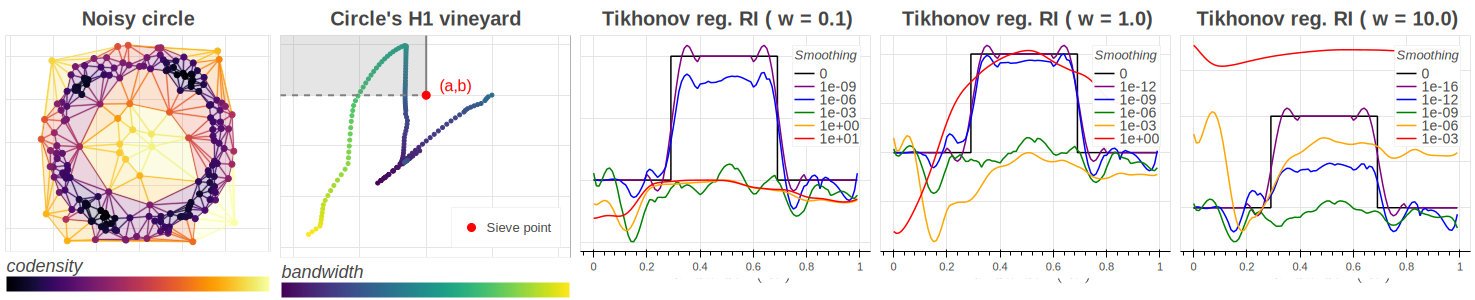
\includegraphics[width=\textwidth]{codensity_ex}
	\caption{From left to right: Delaunay complex $K$ realized from point set $X \subset \mathbb{R}^2$ sampled with multiple types of noise around $S^1$ (colored by codensity at optimal $\alpha^\ast \approx 1/2$); codensity vineyard  of $(K, f_\alpha)$ across varying bandwidths $\alpha$ and a fixed sieve point $(a,b) \in \Delta_+$; Tikhonov regularizations $\hat{\beta}_p^{a,b}(\alpha)$ at varying regularization ($\tau$) and sign width ($\omega$) values. Observe lower values of $\tau$ lead to approximations closer to the rank (black) at the cost of smoothness, while larger values can yield very smooth albeit possibly uninformative relaxations. 
	}\label{fig:codensity_opt}
%	Some choices of $(\tau, \omega)$ lead to continuous and differentiable functions with maxima matching $\alpha^\ast$ }
\end{figure}

 Consider a Delaunay complex $K$ realized from a point set $X \subset \mathbb{R}^2$ sampled around $S^1$ affected by both Hausdorff noise and strong outliers, shown in Figure~\ref{fig:codensity_opt}.
One approach to detect the presence of $S^1$ in the presence of such outliers is maximize $\beta_p^{a,b}(\alpha)$ for some appropriately chosen $(a,b)\in \Delta_+$ over the pair $(K, f_\alpha)$, where $f_\alpha : X \to \mathbb{R}_+$ is a kernel (co)-density estimate:
%bandwidth $\alpha^\ast$ maximizing the persistent Betti number  of 
%the sublevel sets $\hat{f}_h^{-1}((-\infty, t]) \subseteq X$ of $K$  and the choice of a smooth kernel function $\mathcal{K}_h : \mathbb{R} \to \mathbb{R}_+$.
%\begin{equation}
%	
%%	(K, f_h) = \{ \, \sigma \subset X : \max \hat{f}_h(\sigma) \leq t \, \}
%\end{equation}
\begin{equation}\label{eq:betti_opt}
	\alpha^\ast = \argmax_{\alpha \in \mathbb{R}} \; \beta_p^{a,b}(K, f_\alpha), \quad \text{ where } f_\alpha(x) = \frac{1}{n\alpha} \sum_{i} C(\mathcal{K}) - \mathcal{K}_\alpha(x_i - x)
\end{equation}
where $C(\mathcal{K}_\alpha)$ is a normalizing constant that depends on the bandwidth-parameterized kernel, $\mathcal{K}_\alpha$. 
Intuitively, if there exists a choice of bandwidth $\alpha^\ast$ which distinguishes strong outliers from Hausdorff noise clustered around $S^1$, then that choice of bandwidth should exhibit a highly persistent pair $(a^\ast, b^\ast) \in \mathrm{dgm}_1(K, f_{\alpha^\ast})$. 
%In contrast, the limiting cases $\alpha \to 0$ and $\alpha \to 1$ fails to distinguish large differences in such outliers. 
If the corner point $(a,b)$ captures this occurrence and $\lvert a-b \rvert$ is large enough, we expect $\beta_p^{a,b}(\alpha) = 1$ near the optimal bandwidth $\alpha^\ast$---matching the first Betti number of $S^1$---and $0$ otherwise.
%for bandwidth choices that cannot distinguish the points packed densely around $S^1$ against the strong outliers. 

In Figure~\ref{fig:codensity_opt}, we depict the vineyard of $\mathrm{dgm}_1$ of a simple Delaunay complex and codensity pair $(K, f_\alpha)$, along with the sieve point $(a,b)$ and the region wherein $S^1$ is accurately captured by persistence. 
As $\beta_p^{a,b}$ is an integer-valued invariant, it is discontinuous and difficult to optimize; in contrast, we know from Proposition~\eqref{prop:operator_props} that we can obtain a continuous and differentiable relaxation of $\beta_p^{a,b}$ by replacing $\beta_p^{a,b} \mapsto \hat{\beta}_p^{a,b}$ in~\eqref{eq:betti_opt}, enabling the use of first-order optimization techniques.
By using the Tikhonov regularization from~\eqref{eq:tikhonov_1}, we obtain continuously varying objective curves from $\hat{\beta}_p^{a,b}(\alpha; \tau)$ which are guaranteed to have the same maxima as $\beta_p^{a,b}(\alpha)$ as $\tau \to 0$, as shown in Figure~\ref{fig:codensity_opt}. 
Practical optimization of these types of objective surfaces can be handled via \emph{iterative thresholding}, a technique which alternates between gradient steps to reduce the objective and thresholding steps to enforce the rank constraints~\cite{}.
We leave the tuning of such optimizers to future work. 
% between linearioptimizing a given liendecreasing  
%use iterative optimization methods, such as iterative sparse thresholding... 

% --- APPLICATION: Topology-guided simplification ----
\subsection*{Topology-guided simplification}
In many 3D computer graphics applications, one would like to simplify a given simplicial or polygonal mesh embedded in $\mathbb{R}^3$ so as to decrease its level of detail (LOD) while retaining its principal geometric structure(s).   
Such simplifications are often necessary to improve the efficiency of compute-intensive tasks that depend on the size of the mesh (e.g. rendering).
Though many simplification methods developed to preserve geometric criteria---such as curvature, co-planarity, or distance---are now well known (see~\cite{heckbert1997survey} for an overview),
by comparison \emph{topology-preserving} simplification procedures are relatively sparse, especially for higher embedding dimensions. Moreover, such procedures are often limited due to the fact that they restrict to operations that preserve \emph{local} notions of topology, such as the genus of a feature's immediate neighborhood or the property of being a manifold; such procedures are known to greatly limit the amount of detail decimation algorithms can remove~\cite{}. 
%there many applications where one is concerned with preserving notions of ``topology,'' such as neighboring connectivity or the number of `holes' in the mesh, or ~\cite{} 
%facet merging, face decimation and energy minimization in

\begin{figure}[t]
	\includegraphics[width=\textwidth]{elephant_sparsify}
	\caption{(Top) Meshes filtered and colored by eccentricity at varying levels of simplification; (middle) their diagrams and topological constraints; (bottom) simplification thresholds tested by an exponential search, on a logarithmic scale. The color/shape of the markers indicate whether the corresponding meshes meet (green triangle) or do not meet (red x) the topological constraints of the sieve---the gray marker identifies the original mesh (not used in the search). Black dashed circles correspond with the meshes in the top row. 
	In this example, the four rectangular-constraints ensure the simplified elephants have four legs, one trunk, two ears, and two tusks---and that these features have certain minimal persistence $\delta> 0$. 
%	and that these features appear as persistent classes in $\mathrm{dgm}_1(K)$. 
	}
\end{figure}

As a prototypical application of our proposed relaxation, we re-visit the mesh simplification problem under \emph{persistence-based} constraints.
%as is done in e.g.~\cite{fugacci2020topology}.
%One motivation for the practical persistence-based constraints 
In contrast to~\cite{fugacci2020topology}, however, we forgo the use of persistence-preserving operations (which is specialized only for 2-manifolds in $\mathbb{R}^3$) and instead opt for a simpler strategy: 
we perform binary search on a given sequence of simplifications, settling on the largest simplification found. 
That is, assume we have as input a set of simplicial maps: 



we assume the set of topological constraints are given as input via a set of pairs $\{\, (R_1, c_1), (R_2, c_2), \dots, (R_h, c_h)\,\}$, where each $R_i \subset \Delta_+$ prescribing rectangular areas of wherein a multiplicity constraint on the persistence is imposed; we then seek to minimize the size of the mesh $K$ 
%and we compare the quadric decimation on a mesh using local topology-preserving vs a simple exponential search on the set $[0, {n \choose 3})$, the input parameter to the simplification.
 
%$$\mathcal{R}_{\mathrm{constr}} \subset \Delta_+$$
%We then consider the optimation problem: 
$$
\begin{aligned}
\min_{\alpha \in \mathbb{R}} \quad &  \#\,\mathrm{card}(K_\alpha^p)	\\
\textrm{s.t.} \quad & \mu_p^{R_i}(K_\alpha, f_\alpha) = c_i, \quad \forall \; R_i \in \mathcal{R}
%\mathrm{dgm}_p(K, f_\alpha) \cap \mathcal{R}
\end{aligned}
$$
In other words, the set 

%which relies on persistence-preserving operations (such as vertex removals and edge flips) that have bounded changes in persistence as measured by the bottleneck distance, we expect the topological constraints to be encoded by the sieve. 

%The issue with persistence-based based constraints is, of course, computation. Computing the bottleneck distance is difficult, and maintaining a persistence diagram under 
%
%Here, we consider a 3D mesh library of animals pose data~\cite{chazal2009gromov}. As these are high quality meshes, one may be interested in geometric simplifications, such as quadric decimation procedure, which takes as input the number of triangles $n_2$ desired in the output. 
%
%A priori, it is unclear how to set $k$---however, since the taxonomical classification of these meshes are known, one simple criterion one might want to preserve the existence of major extremities, such as limbs, tails, and/or horns. 

%In many applications, simplifications defined solely using geometric properties is not enough---often, such simplifications are preferred to be \emph{topology-preserving} in some sense, e.g. edge collapses must preserve neighboring connectivity or the number of holes.
%Though such operations are often critical to..., they are inherently \emph{local} conditions. With the exception of very simple properties (e.g. connectedness, the Euler characteristic, etc.) it is often far too expensive to ensure \emph{global} topological properties of shapes are preserved under incremental simplification procedures, either because the properties themselves are expensive to check (per simplifying operation) or because the existing simplification procedure cannot ensure such guarantees. 


% --- APPLICATION: Topology-guided simplification ----
\subsection*{Manifold detection from image patches}
A common hypothesis is that high dimensional data tend to lie in the vicinity of an embedded, low dimensional manifold or topological space. An exemplary demonstration of this is given in the analysis by Lee et al.~\cite{lee2003nonlinear}, who explored the space of high-contrast patches extracted from Hans van Hateren's still image collection,\footnote{See \url{http://bethgelab.org/datasets/vanhateren/} for details on the image collection.} which consists of $\approx 4\text{,}000$ monochrome images depicting various areas outside Groningen (Holland). 
Originally motivated by discerning whether there existed clear qualitative differences in the distributions of patches extracted from images of different modalities, such as optical and range images, Lee et al.~\cite{lee2003nonlinear} were interested in exploring how high-contrast $3 \times 3$ image patches were distributed in pixel-space with respect to predicted spaces and manifolds.
Formally, they measured contrast using a discrete version of the scale-invariant Dirichlet semi-norm:
$$ \lVert x \rVert_D = \sqrt{\sum_{i \sim j}(x_i - x_j)^2} = \sqrt{x^T D x}$$
where $D$ is a fixed matrix whose quadratic form $x^T D x$ applied to an image $x \in \mathbb{R}^9$ is proportional to the sum of the differences between each pixels 4 connected neighbors (given above by the relation $i \sim j$).
%Their research was .
By mean-centering, contrast normalizing, and``whitening'' the data via the Discrete Cosine Transform (DCT), they show a convenient basis for $D$ may be obtained via an expansion of 8 certain non-constant eigenvectors: 
\begin{center}
	\includegraphics[width=0.80\textwidth]{dct_basis_trimmed} 
\end{center}
Since these images are scale-invariant, the expansion of these basis vectors spans the 7-sphere, $S^7 \subset \mathbb{R}^8$. Using a Voronoi cell decomposition of the data, their distribution analysis suggested that the majority of data points concentrated in a few high-density regions. 

In follow-up work, Carlsson et al.~\cite{carlsson2008local} used persistent homology to find the distribution of high-contrast $3 \times 3$ patches is actually well-approximated by a Klein bottle $\mathcal{M}$---around 60\% of the high-contrast patches from the still image data set lie within a small neighborhood around $\mathcal{M}$ accounting for only 21\% of the 7-sphere's volume. 
Though a certainly remarkable result, if one was not aware of the analysis done by~\cite{lee2003nonlinear, carlsson2008local}, it would not be immediately clear a priori how to reproduce the discovery in the more general setting; e.g. how does one determine which topological space is a viable model for image patches? 
Indeed, armed with both efficient persistent homology software and refined topological intuition, Carlsson still needed to perform extensive point-sampling, preprocessing, and model fitting techniques in order to substantiate the Klein bottle was an appropriate space for the distribution of $3 \times 3$ patches~\cite{carlsson2008local}.
One of the motivations of \emph{multi-parameter persistence}---which filters the data along multiple dimensions---is to eliminate the necessity of such extensive preprocessing.
%Unfotunately, such preprocessing is necessary is due to persistent homology's aforementioned instability with respect to strong outliers. 
% This can be further verified empirically by e.g. using the iterative, meanshift-like procedure described in~\cite{carlsson2008local} to fit a parameterization of the model in question to the data. 


%It is widely considered 
%In contrast to the 1-parameter setting, a multi-parameter persistence approach that accounts for the local density of points to be able to identify the presence of the Klein bottle, even in the midst of outliers. 
%To demonstrate this, we consider 

\begin{center}
	\includegraphics[width=0.40\textwidth]{hilbert_unmarked} 
	\includegraphics[width=0.40\textwidth]{pers5} 
\end{center}



%Unfortunately, compute barriers tend to bar the use of multi-parameter persistence in practice: the size of a general $n$-D filtrations can be enormous~\cite{}. Though much work has been done on approximating certain multi-parameters invariants (such as the fibered barcode), exact computation of many of the invariants associated with general multi-parameter persistence modules is widely considered intractable, see~\cite{} for a survey. 


%The degree to which multi-parameter persistence simplifies this exploratory phase cannot be understated: we believe multi-parameter persistence has a larger role to play in manifold learning. 





%In these contexts, the topology-related measure being preserved a
%such as connectedness or the preservation of certain holes across face collapses~\cite{}. 
% In the former case, topologically critical changes are permitted unhindered, while in latter is restricted to preserving are purely local notions of topology, such as connectedness or the preservation of certain holes across face collapses~\cite{}. 

% --- APPLICATION 1: Fast spectral computation ---


%For example, weighting edges of the graph Laplacian originally studied by Kirchoff typically has natural interpretations as electrical \emph{conductance}/\emph{resistance} that arise electrical circuit networks, due to Ohms law and conservation of flow. 
%By normalizing 
%\emph{normalized} graph Laplacian arises naturally as a \emph{diffusion operator} in the study of transition probabilities. 
%As another example, the signless Laplacian...


% --- APPLICATION: Continuous Persistent Betti Curves (PBCs) as Shape Signatures --- 
% Benefits of rank(A) \approx < nuclear norm of A >
%\subsection*{Application: Relaxation}
%\subfile{spectral_relaxation}

% --- APPLICATION 2: Directional transforms as Shape Signatures ---- 
%\subsection*{Shape comparison}
%In general, both combinatorial and topological aspects of a given topological space are encoded in the spectra of Laplacian operators. 
%Through their null-space, combinatorial Laplacians encode a complexes basic topology via its homology groups---this is identical for most of the Laplace operators, whether they are normalized, weighted, signless, and so on~\cite{}.
%In contrast, these operators differ in the nonzero part of the spectrum, which encode specific geometric information in addition to topological properties. 
%
% 
%\begin{figure}
%	\centering
%	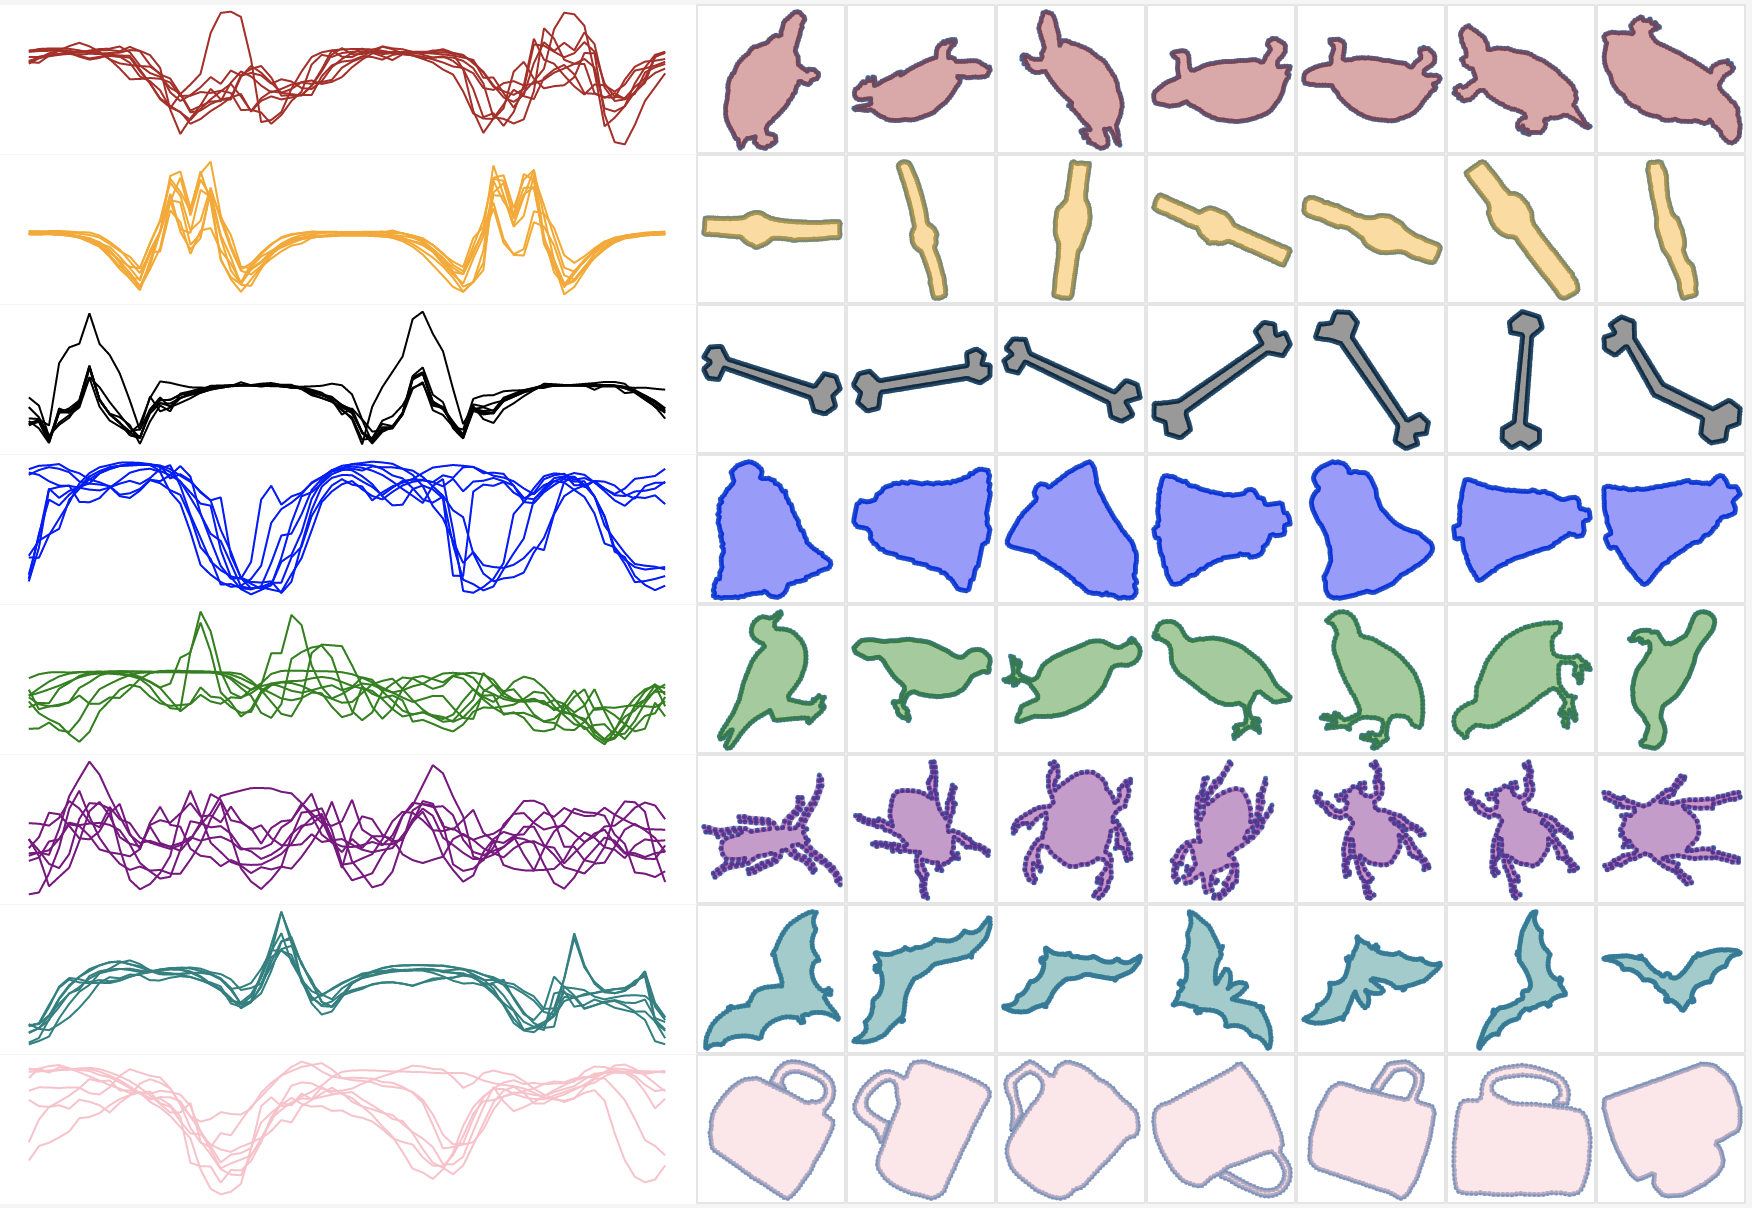
\includegraphics[width=0.6\textwidth]{shape_signatures}
%\end{figure}

\section{Conclusion \& Future Work}
Interestingly, our results also imply the existence of an efficient output-sensitive algorithm for computing $\Gamma$-persistence pairs with at least ($\Gamma >0$)-persistence (via~\cite{chen2011output}) that requires the operator $x \mapsto \partial x$ as its only input, which we consider to be of independent interest. 
\\
\noindent \textbf{Limitations:} it is worth remarking that there are few limitations to the proposed work that may prevent its practical use on certain types of problems. In particular, the most significant limitations we encountered in this effort were related to (a) tuning the degree of regularization of the chosen matrix function, and (b) scaling up the implementation of the rank function approximation. 
As is evident by Figure... due to the combinatorial nature of the Betti number from, obtain the exact dimension of each tmer in ~\ref{} requires shrinking $\epsilon$ to a factor of $O(1 / n)$, which itself is implies the $(1 \pm \epsilon)$-approximation from~\cite{} require only of the order of $O(mn)$ when $\log(\eta^{-1})$ is treated as a small constant. This is not too surprising, as it in fact matches out the exact bound from~\ref{}, however we consider it a limitation nonetheless. 

The second major limitation, is the fact that the scalability of our proposed framework depends heavily on the scalabality of the chosen rank implementation itself. Indeed, due to Corollary~\ref{}, we observed empirically that computing the rank computation itself accounts for upwards of 90\%+ of the computation for fixed complexes (especially those not subject to the optimization from~\ref{}). On the other hand, 

\bibliography{pbsig_bib}
\bibliographystyle{plain}

\newpage 

\appendix
\section{Appendix}

%
\subsection*{Expanded Intro}
% Gromov-Hausdorff Stable Signatures for Shapes using Persistence
Though homology is primarily studied as a topological invariant, the fact that persistent homology encodes both topological and geometric information in its diagram has motivated its use not only as a shape descriptor but also as a metric invariant. 
Metric invariants, or ``signatures,'' are commonly used in metric learning to ascertain whether two comparable data sets $X, Y$ represent the same object---typically up to a some notion of invariance.
%the similarity of thdistances $d(X,Y) = 0$.
One mathematically attractive model for measuring the dissimilarity between shapes/datasets is the Gromov-Hausdorff (GH) distance $d_{\text{GH}}((X, d_X), (Y,d_Y)$ between compact metric spaces $(\mathcal{X}, d_X), (\mathcal{Y}, d_Y)$: by altering the choice of metric $(d_X, d_Y)$, the corresponding metric-distance $d_{\text{GH}}$ can be adapted to a chosen notion of invariance~\cite{} or to increase its discriminating power~\cite{}. 
Though it is NP-hard to compute~\cite{}, the GH distance defines a metric on the set of isomorphism classes of compact metric spaces endowed with continuous real-valued functions, justifying its study as a mathematical model for shape matching and metric learning. 
Moreover, it is known that the bottleneck distance between persistence diagrams over Rips filtrations $R(X, d_X), R(Y, d_Y)$ is a tight, stable lower bound on the GH distance~\cite{}. 
Indeed, Solomon et al~\cite{} showed distributed persistence invariants characterize the quasi-isometry type of the underlying space, allowing one to provably interpolate between geometric and topological structure.
% curvature sets?

%For example, it is often the case one wishes to construct a (pseudo-)mettric on a given space of objects for comparison or classification purposes. Though the information contained in some topological invariants is immense, strictly topological information is often not enough to distinguish things---geometry is needed. 
%In many ways, persistence is an important tool in the widely studied \emph{manifold hypothesis} problem, wherein $\mathcal{X}$ is a compact Riemannian submanifold of Euclidean space, and $X \subset \mathcal{X}$ is sampled according to the intrinsic uniform distribution.
% since $\beta_p^{i,j}(K; \mathbb{F}) = \mathrm{dim}(H_p^i \to H_p^j)$.
%Despite being information rich, persistence diagram reflect persistent homology group, and homology groups as a topological invariant are quite weak. 
%An exemplary case of this, consider the Euler characteristic $\chi(X) = V - E + F$: by itself is rich enough to distinguish connectedness of space, though obviously as a single number its discriminatory power is quite limited. 
%To increase discriminatory power, a given set of complexes $K$ are typically filtered with respect to a direction $f : K \to \mathbb{R}$, and then $\chi$ is calculated on each sub level set, producing a Euler characteristic curve (ECC).
% By choosing $f$ more carefully, such as by filtering with respect to curvature, one can imbue the corresponding featurization to depend more on the geometry of the underlying embedding~\cite{}.
% Recent work suggests that families of ECCs contain sufficient enough information to reconstruct the input perfectly, or to construct distance metrics on shape space.  
% More generally, the directional transform... PHT.. 
%This is very much so an exciting and active area of research, more recent work has extended this, yielding a foundation for shape analysis on shape space. 

Though theoretically well-founded and information dense, persistence diagrams come with their own host of practical issues: they are sensitive to strong outliers, far from injective, and their de-facto standard computation exhibits high algorithmic complexity. 
Moreover, the space of persistence diagrams $\mathcal{D}$ is a Banach space, preventing one from doing even basic statistical operations, such as averaging~\cite{}. 
As a result, many researchers have focused on extending, enhancing, or otherwise supplementing persistence diagrams with additional information. 
% template functions...
Turner et al~\cite{} proposed associating a collection a shape descriptors with a PL embedded $X \subset \mathbb{R}^d$---one descriptor for each point on $S^{d-1}$---which they called a \emph{transform}. 
More exactly, suppose both the data $X$ and its geometric realization $K$ are PL embedded in $\mathbb{R}^d$ and has centered and scaled appropriately.
The main theorem in~\cite{} is that associating a persistence diagram, or even a simpler descriptor such as the Euler characteristic, for every point on $S^{d-1}$ is actually sufficient information to theoretically reconstruct $K$. 

 Missing from the above work is the are two important directions: how do you configure such transforms to retain the important topological/geometric information and discard irrelevant information, and (2) how may we efficiently compute them? 
The former question is synonymous with choosing the invariance model in the GH framework, which seems to be highly domain specific. 
% TODO: template functions
 In the latter case, though we know the number of directions is bounded~\cite{}, the bound is simply too high to be of any practical use. While there are efficient algorithms for both the ECC and persistence computations in static settings, the state of the art in parameterized settings is non-trivial and ongoing research area.



\subsection{Combinatorial Laplacians}\label{sec:laplacian_theory}
% "Many combinatorial operations that one can perform on a simplicial complex do not affect its homology typically leave characteristic traces in the spectrum of a suitable Laplace operator. In the weighted case, there is additional geometric information that likewise influences the spectrum." 
The natural extension of the graph Laplacian $L$ to simplicial complexes is the \emph{$p$-th combinatorial Laplacian} $\Delta_p$, whose explicit matrix representation is given by: 
\begin{equation}
	\Delta_p(K) = 
	\underbrace{\partial_{p\+1} \circ \partial_{p\+1}^T}_{L_p^{\text{up}}} + \underbrace{\partial_{p}^T  \circ  \partial_{p}}_{L_p^{\text{dn}}} 
%	\simeq H() 
\end{equation}
\noindent Indeed, when $p = 0$, $\Delta_0(K) = \partial_1 \partial_1^T = L$ recovers the graph Laplacian. 
As with boundary operators, $\Delta_p(K)$ encodes simplicial homology groups in its nullspace, a result known as the discrete Hodge Theorem~\cite{}: 
\begin{equation}\label{eq:laplace_hom}
	\tilde{H}_p(K; \mathbb{R}) \cong \mathrm{ker}(\Delta_p(K)), \quad \beta_p = \mathrm{nullity}(\Delta_p(K))
\end{equation}
The fact that the Betti numbers of $K$ may be recovered via the nullity of $\Delta_p(K)$ has been well studied (see e.g. Proposition 2.2 of~\cite{}). 
In fact, as pointed out by~\cite{}, one need not only consider $\Delta_p$ as the spectra of $\Delta_p$, $L_p^{\text{up}}$, and $L_p^{\text{dn}}$ are intrinsically related by the identities:
\begin{equation}\label{eq:lap_spectra_conn}
	\Lambda(\Delta_p(K)) \doteq \Lambda(L_p^{\text{up}}) \stackrel{\cdot}{\cup} \Lambda(L_p^{\text{dn}}), \quad \quad \Lambda(L_p^{\text{up}}) \doteq \Lambda(L_{p+1}^{\text{dn}})
\end{equation}
where $A \doteq B$ and $A \stackrel{\cdot}{\cup} B$ denotes equivalence and union between the \emph{non-zero} elements of the multisets $A$ and $B$, respectively.
Moreover, all three operators $\Delta_p$, $L_p^{\text{up}}$, and $L_p^{\text{dn}}$ are symmetric, positive semidefinite, and compact---thus, for the purpose of estimating $\beta_p$, it suffices to consider only one family of operators.
%Indeed, using the analysis done~\cite{}, the number of non-zero 


%for substitution into step (4) of the outline from section~\ref{sec:rank_invariant_summary}.
%Unfortunately, various difficulties arise when adapting combinatorial Laplacians to the the \emph{persistent} case. 
%One might expect that restricting... one would obtain, however this is not true, see the counter-example given in~\cite{}. 
%Recent work by Mémoli, Wan, and Wang has established an important connection between combinatorial Laplacians and persistence, including a matrix representative whose kernel encodes $\beta_p^{i,j}$. However  

%However, the non-zero part of their spectra varies significantly both in the choice of operator and weight function.
%be used as a rank invariant 
%As our spectral rank approximation~\eqref{def:smooth_mu} is driven entirely by this non-zero portion, it is pertinent to consider viable choices and their ramifications.
%Indeed, normalization and symmetrization are themselves weighting schemes. 
%Indeed, it is known that the spectra of Laplacians reflects the geometric aspects of about intersection pattern 
%Thus, we will use the terms \emph{weight function} and \emph{scalar product} interchangeably. 
To translate the continuity results from definition~\ref{def:smooth_mu} to any of the Laplacian operators above, we must consider weighted versions. 
Here, a \emph{weight function} is a non-negative real-valued function defined over the set of all faces of $K$:
\begin{equation}\label{eq:weight_func} % isn't this the same as w: K \to R_+ ??
	w : K \to \mathbb{R}_+
%	w: \bigcup_{p=-1}^{\mathrm{dim}(K)} K^p \to \mathbb{R}_+
\end{equation}
%The choice of weight function is tightly coupled to the choice of scalar product on the coboundary vector space $C^p(K, \mathbb{R})$. 
The set of weight functions and the choice of scalar product on $C^p(K, \mathbb{R})$ wherein elementary cochains are orthogonal are in one-to-one correspondence~\cite{} (see Appendix~\ref{sec:inner_products}). In this way, we say that the weight function \emph{induces} an inner product on $C^p(K, \mathbb{R})$:
%It can be shown that for any choice of inner product on $C^p(K, \mathbb{R})$, there exists a positive weight function $f: K \to \mathbb{R}_+ \setminus \{0\}$ satisfying: 
\begin{equation}
	\langle \, f, g \, \rangle_{w} = \sum\limits_{\sigma \in K^p} w(\sigma) f([\sigma]) g([\sigma])
\end{equation}
Moreover, Laplacian operators are uniquely determined by the choice of weight function.  
This correspondence permits us to write the matrix representation of $\Delta_p$ explicitly: 
\begin{equation}\label{eq:weighted_up_laplace}
	\Delta_p(K, w) \triangleq  W_p^{+} \partial_{p+1} W_{p+1} \partial_{p+1}^T \, + \,  \partial_{p}^T W_p^{+} \partial_p W_{p+1} 
\end{equation} 
where $W_p = \mathrm{diag}(\{ \, w(\sigma_i) \, \}_{i=1}^n)$ represents a non-negative diagonal  matrices restricted $\sigma \in K^p$ and $W^+$ denotes the pseudoinverse. 
Note that~\eqref{eq:weighted_up_laplace} recovers~\eqref{eq:comb_lap} in the case where $w$ is the constant map $w(\sigma) = 1$, which we call the \emph{unweighted} case. 
%Note that $L_p^{\textrm{up}}$ is uniquely determined by its restriction to $K^{p+1}$ and $L_p^{\textrm{dn}}$ by its restriction to $K^p$. Thus, noting~\eqref{eq:lap_spectra_conn}, we may  consider whichever is more computationally convenient. 


Unfortunately, various difficulties arise with weighting combinatorial Laplacians with non-constant weight functions, such as asymmetry, scale-dependence, and spectral instability.
Indeed, observe that in general neither terms in~\eqref{eq:weighted_up_laplace} are symmetric unless $W_p = I_n$ (for $L_p^{\text{up}}$) or $W_{p+1} = I_m$ (for $L_p^{\text{dn}}$). 
%$W_p^{-1} \partial_{p+1} W_{p+1} \partial_{p+1}^T$ 
However, as noted in~\cite{memoli2022persistent}, $L_p^{\text{up}}$ may be written as follows: 
\begin{equation}\label{eq:l_up}
	L_p^{\text{up}} = W_p^{+} \partial_{p+1} W_{p+1} \partial_{p+1}^T  = W_p^{+/2} \big( W_p^{+/2}  \partial_{p+1} W_{p+1} \partial_{p+1}^T W_p^{+/2}  \big ) W_p^{1/2} 
\end{equation}
Since~\eqref{eq:l_up} is of the form $W^{+} P W$ where $P \in S_n^+$ and $W$ is a non-negative diagonal matrix, this rectifies the symmetry problem.
Towards bounding the spectra of $L_p^{\text{up}}$, Horek and Jost~\cite{} propose \emph{normalizing} $\Delta_p$ by augmenting $w$'s restriction to $K^p$: 
\begin{equation}
	w(\tau) = \sum\limits_{\tau \in \partial(\sigma) }w(\sigma) \quad \forall \; \tau \in K^{p}, \, \sigma \in K^{p+1}
\end{equation}
Substituting the weights of the $p$-simplices in this way is equivalent to mapping $W_p \mapsto \mathcal{D}_p$ where $\mathcal{D}_p$ is the \emph{diagonal degree matrix}. The corresponding substitution in~\eqref{eq:l_up} yields the \emph{weighted combinatorial normalized Laplacian} (up-)operator:
\begin{align*}\label{eq:normalized_up_lap}
	 \mathcal{L}_p^{\text{up}} = (\mathcal{D}_p)^{+/2} \partial_p W_{p+1} \partial_p^T (\mathcal{D}_p)^{+/2} = \mathcal{I}_n - \mathcal{A}_p^{\text{up}} \numberthis
\end{align*}
where $\mathcal{A}_p^{\text{up}}$ is a weighted adjacency matrix, and $\mathcal{I}_n$ is the identity matrix with $\mathcal{I}(\tau) = \mathrm{sign}(w(\tau))$ (see Section~\ref{sec:comb_lap}). The primary benefit of this normalization is that it guarantees $\Lambda( \mathcal{L}_p^{\text{up}}) \subseteq [0,p+2]$ for any choice of weight function, from which one obtains several useful implications, such as tight bounds on the spectral norm~\cite{}. 
The same results holds for up-, down-, and combinatorial Laplacians.
Moreover, as we will show in a subsequent section, one obtains stability properties with degree-normalization not shared otherwise. 

\begin{remark}
	Compared to~\eqref{eq:l_up}, is it worth remarking that one important quality lost in preferring $\mathcal{L}_p^{\text{up}}$ over $L_p^{\textrm{up}}$ is diagonal dominance. 
	%may no longer be diagonally dominant (though it is PSD). 
\end{remark}

%For all the reasons given above, we exclusively consider the normalized combinatorial Laplacian operator for the remainder of the paper. Moreover, using the spectral connection between boundary and Laplacian operators, we will exclusively consider spectral rank invariants of the form: 

\subsection*{Laplacian matvec}\label{app:lap_matvec}
We first recall the characteristics of the graph Laplacians $x \mapsto Lx$ operation. 
Given a simple undirected graph $G = (V, E)$, let $A \in \{0,1\}^{n \times n}$ denote its binary adjacency matrix satisfying $A[i,j] = 1 \Leftrightarrow i \sim j$ if the vertices $v_i,v_j \in V$ are adjacent in $G$, and let $D = \mathrm{diag}(\{ \, \mathrm{deg}(v_i) \, \})$ denote the diagonal \emph{degree} matrix, where $\mathrm{deg}(v_i) = \sum_{j \neq i} A[i,j]$.
The \emph{graph Laplacian}'s adjacency, incidence, and element-wise definitions are: 
\begin{equation}
L = D - A = \partial_1 \circ \partial_1^T \, , \quad\quad
	L\,[i,j] = \begin{cases}
		\mathrm{deg}(v_i) & \text{ if } i = j \\
		-1 & \text{ if } i \sim j \\
		0 & \text{ if } i \nsim j
	\end{cases}
\end{equation}
%It is well known that $L$ is symmetric, positive semi-definite, and has a combinatorial structure that captures the connectivity structure of $G$~\cite{newman2001laplacian}. 
Furthermore, by using the adjacency relation $i \sim j$ as in~\cite{chung1997spectral}, the linear and quadratic forms of $L$ may be succinctly expressed as:
\begin{flalign}\label{eq:lap_quad_from}
	(\, \forall \, x \in \mathbb{R}^n \,)  & & \quad\quad\quad 
	(Lx)_i = \mathrm{deg}(v_i) \cdot x_i - \sum\limits_{i \sim j} x_j \, , \quad \quad &
	 x^T L x = \sum\limits_{i \sim j} (x_i - x_j)^2  & &&
%	  x^T L x = \sum\limits_{i \sim j} f(v_i, v_j) (x_i - x_j)^2  & &&
\end{flalign}
If $G$ has $m$ edges and $n$ vertices taking labels in the set $[n]$, computing the product from~\eqref{eq:lap_quad_from} requires just $O(m)$ time and $O(n)$ storage via two edge traversals: one to accumulate vertex degrees and one to remove components from incident edges. By precomputing the degrees, the operation reduces further to a single $O(n)$ product and $O(m)$ edge pass, which is useful when repeated evaluations for varying values of $x$ are necessary. 
%As we show below, generalizing this procedure when $p > 0$ requires .
%, as the orientations of $[\sigma] \in K^{p+1}$ change the sign of the off-diagonal entries in $L_p^\ast$. 
%In particular, writing down a succinct expression for $x \mapsto L_p^{\textrm{up}} x$ (or $x \mapsto L_p^{\textrm{dn}} x$) requires a generalization of the notion of path-connectedness between $p$-simplices, as well as knowledge of the orientation of every simplex to evaluate the sign..

To extend the two-pass algorithm outlined above when $p > 0$, we first require a generalization of the connected relation from~\eqref{eq:lap_quad_from}.
 Denote with $\mathrm{co}(\tau) = \{ \, \sigma \in K^{p+1} \mid \tau \subset \sigma \, \}$ the set of proper cofaces of $\tau \in K^p$, or \emph{cofacets}, and the (weighted) \emph{degree} of $\tau \in K^p$ with: 
$$\mathrm{deg}_w(\tau) = \sum_{\sigma \in \mathrm{co}(\tau)} w(\sigma) $$
Note setting $w(\sigma) = 1$ for all $\sigma \in K$ recovers the integral notion of degree representing the number of cofacets a given $p$-simplex has. 
Now, since $K$ is a simplicial complex, if the faces $\tau, \tau'$ share a common cofacet $\sigma \in K^{p+1}$, this cofacet $\{\sigma\} = \mathrm{co}(\tau) \cap \mathrm{co}(\tau')$ is in fact \emph{unique}~\cite{goldberg2002combinatorial}. 
Thus, we may use a relation $\tau \overset{\sigma}{\sim} \tau'$ to rewrite the operator from~\eqref{eq:l_up} element-wise: 
\begin{align}\label{eq:up_laplace_theory}
	 L_p^{\text{up}}(\tau, \tau')= \begin{cases}
		 \mathrm{deg}_w(\tau) \cdot w^{+}(\tau) & \text{ if } \tau = \tau' \\ 
%		\mathrm{deg}(\tau_i) & \text{ if } i = j \\ 
		s_{\tau, \tau'} \cdot  w^{+/2}(\tau) \cdot w(\sigma) \cdot w^{+/2}(\tau') & \text{ if } \tau \overset{\sigma}{\sim} \tau' \\
		0 & \text{ otherwise} 
	\end{cases}
\end{align}
where $s_{\tau, \tau'} = \mathrm{sgn}([\tau], \partial[\sigma]) \, \cdot \, \mathrm{sgn}([\tau], \partial[\sigma])$. Ordering the $p$-faces $\tau \in K^p$ along a total order and choosing an indexing function $h : K^p \to [n]$ enables explicit computation of the corresponding matrix-vector product: 
\begin{equation}\label{eq:l_up_matvec}
	(L_p^{\textrm{up}} \, x)_i =  \mathrm{deg}_w(\tau_i) \cdot w^{+}(\tau_i) \cdot x_i + w^{+/2}(\tau_i) \sum\limits_{\tau_j \overset{\sigma}{\sim} \tau_i} s_{\tau_i, \tau_j} \cdot x_{j} \cdot w(\sigma) \cdot w^{+/2}(\tau_j) 
\end{equation}
Observe~\eqref{eq:l_up_matvec} can be evaluated now via a very similar two-pass algorithm as described for the graph Laplacian if the simplices of $K^{p+1}$ can be quickly enumerated and the indexing function $h$ can be efficiently evaluated. 

Below is pseudocode outlining how to evaluate a weighted (up) Laplacian matrix-vector multiplication built from a simplicial complex $K$ with $m = \lvert K^{p+1} \rvert$ and $n = \lvert K^{p} \rvert$ in essentially $O(m)$ time when $m > n$ and $p$ is considered a small constant. 
Key to the runtime of the operation being essentially linear is the constant-time determination of orientation between $p$-faces ($s_{\tau, \tau'}$)---which can be inlined during the computation---and the use of a deterministic $O(1)$ hash table $h : K^{p} \to [n]$ for efficiently determining the appropriate input/output offsets to modify ($i$ and $j$). 
Note the degree computation occurs only once. 

\begin{algorithm}[H]\label{alg:lap_matvec}
\renewcommand{\algorithmicensure}{\textbf{Optional:}}
%\algrenewcommand\algorithmicoptional{\textbf{Output:}}
\caption{\texttt{matvec} for weighted $p$ up-Laplacians in $O(m(p+1)) \approx O(m)$ time ($p \geq 0$)}
\begin{algorithmic}[1]
\Require Fixed oriented complex $K$ of size(s) $N=\lvert K \rvert$, $n = \lvert K^{p}\rvert$, $m = \lvert K^{p+1}\rvert$ 
%\Ensure Weight functions $w_{p+1}: K^{p+1} \to \mathbb{R}_{+}$ and  $w_{p}: K^p \to \mathbb{R}_{+}$
\Ensure Weight arrays $w_{p+1} \in \mathbb{R}_{+}^{m}$ and $w_{p} \in \mathbb{R}_{+}^{n}$
\renewcommand{\algorithmicensure}{\textbf{Output:}}
\Ensure $y = \langle \, L_p^{\mathrm{up}}, x \, \rangle =  (W_p \circ \partial_{p+1} \circ W_{p+1} \circ \partial_{p+1}^T \circ W_p)x$
\State // Precompute weighted degrees $\mathrm{deg}_w$ 
\State Define $h : K^p \to [ \, n \, ]$ 
\State $\mathrm{deg}_w \gets \mathbf{0}$
\For{$\sigma \in K^{p+1}, k \in [m]$}: 
	\For{$\tau \in \partial[\sigma]$}:
   	 	\State $\mathrm{deg}_w[h(\tau)] \gets \mathrm{deg}_w[h(\tau)] + w_p[h(\tau)] \cdot w_{p+1}[k] \cdot  w_{p}[h(\tau)]$
   	\EndFor
\EndFor
\State 
%\State \# Compute Laplacian \texttt{matvec} for $x$ 
\Function{UpLaplacianMatvec}{$x \in \mathbb{R}^n$}
\State $y \gets \mathrm{deg}_w \odot x$ \; \text{(element-wise product)}
%\State $z_{h_p(\tau)} \gets z_{h_p(\tau)} \cdot f(\tau)^2 \quad \forall \tau \in K^p$
\For{$\sigma \in K^{p+1}, k \in [m]$}:
%    $\mathrm{sgn}(\partial[\sigma])$
    \For{$\tau, \ \tau' \in \partial[\sigma] \times \partial[\sigma]$ \textbf{where} $\tau \neq \tau'$}: 
    		\State $s_{\tau, \tau'} \gets \mathrm{sgn}([\tau], \partial[\sigma]) \cdot \mathrm{sgn}([\tau'], \partial[\sigma])$
    		\State $i, \; j \gets \; h(\tau), \; h(\tau')$
    		\State $y_i \gets y_i + s_{\tau, \tau'} \cdot x_{j} \cdot w_p[i] \cdot w_{p+1}[k] \cdot w_p[j]$
    \EndFor 
\EndFor
\State \Return $y$
\EndFunction
\end{algorithmic}
\end{algorithm}

In general, the signs of the coefficients $\mathrm{sgn}([\tau], \partial[\sigma])$ and $\mathrm{sgn}([\tau'], \partial[\sigma])$ depend on the position of $\tau, \tau'$ as summands in $\partial[\sigma]$, which itself depends on the orientation of $[\sigma]$. Thus, evaluation of these sign terms takes $O(p)$ time to determine for a given $\tau \in \partial[\sigma]$ with $\mathrm{dim}(\sigma) = p$, which if done naively via line (12) in the pseudocode~\ref{alg:lap_matvec} increases the complexity of the algorithm. 
However, observe that the sign of their product is in fact invariant in the orientation of $[\sigma]$ (see Remark 3.2.1 of~\cite{goldberg2002combinatorial})---thus, if we fix the orientation of the simplices of $K^p$, the sign pattern $s_{\tau, \tau'}$ for every $\tau \overset{\sigma}{\sim} \tau'$ can be precomputed and stored ahead of time, reducing the evaluation $s_{\tau, \tau'}$ to $O(1)$ time and $O(m)$ storage. 
Alternatively, if the labels of the $p+1$ simplices $\sigma \in K^{p+1}$ are given an orientation induced from the total order on $V$, then we can remove the storage requirement entirely and simply fix the sign pattern during the computation. 

A subtle but important aspect of algorithmically evaluating~\eqref{eq:l_up_matvec} is the choice of indexing function $h: K^p \to [n]$. This map is necessary to deduce the contributions of the components $x_\ast$ during the operation (line (13)). 
While this task may seem trivial as one may use any standard associative array to generate this map, typical implementations that rely on collision-resolution schemes such as open addressing or chaining only have $O(1)$ lookup time in expectation.
Moreover, empirical testing suggests that line (13) in~\ref{alg:lap_matvec} can easily bottleneck the entire computation due to the scattered memory access such collision-resolution schemes may involve. 
%Preliminary benchmarks suggest 
One solution avoiding these collision resolution schemes that exploits the fact that $K$ is fixed is to  build an order-preserving \emph{perfect minimal hash function} (PMHF) $h : K^p \to [n]$. 
It is known how to build PMHF's over fixed input sets of size $n$ in $O(n)$ time and $O(n \log m)$ bits with deterministic $O(1)$ access time~\cite{}. Note that this process happens only once for a fixed simplicial complex $K$: once $h$ has been constructed, it is fixed for every $\mathtt{matvec}$ operation. 
% TODO: mention boissonants data structures


% ----- Laplacian's encoding geometry: https://arxiv.org/pdf/1105.2712.pdf ----
% "In terms of the spectrum, they are given by the dimensions of the eigensets for the eigenvalue 0. This is the same for all the Laplace operators investigated here. These operators, however, differ in the nonzero part of the spectrum, and thereby encode specific combinatorial or geometric features of a (perhaps weighted) simplicial complex in addition to its topological aspects...many combinatorial operations that one can perform on a simplicial complex do not affect its homology; nevertheless, they typically leave characteristic traces in the spectrum of a suitable Laplace operator, and that is what we are trying to explore... in the weighted case, there is additional geometric information that likewise influences the spectrum"

%\subsection*{Directional Transform}
%The canonical interpretation of the information displayed by a persistence diagram is that is summarizes the persistence of the sublevel sets of filtered space. Given a filtration pair $(\, K, f \, )$ where $K$ is a finite simplicial complex and $f : K \to \mathbb{R}$ is a real-valued function, the sublevel sets $\lvert K \rvert_i=f^{-1}(-\infty, i]$ deformation retract to... % say more about stars, homotopy equivalence
% simplexwise-linear function
% http://www.csun.edu/~ctoth/Handbook/chap24.pdf
If $K$ is embedded in $\mathbb{R}^d$, then geometrically $f$ takes on the interpretation of a `height' function whose range yields the `height' of every simplex in $K$. 
%Obviously, this notion of height depends on the embedding of $K$: viewing $K$ (and thus, $X$) from different `directions' induces potentially distinct sublevel sets, 

%Given a simplicial complex $K$ embedded in $\mathbb{R}^d$, 
Let $X \subset \mathbb{R}^d$ denote a data set which can be written as a finite simplicial complex $K$ whose simplices are PL-embedded in $\mathbb{R}^d$. Given this setting,  define the \emph{directional transform} (DT) of $K$ as follows:
\begin{align*}\label{eq:pht}
	\mathrm{DT}(K): S^{d-1} &\to  K \times C(K, \mathbb{R}) \\
	v &\mapsto (K_\bullet, f_v)
\end{align*}
where we write $(K_\bullet, f)$ to indicate the filtration on $K$ induced by $f_v$ for all $\alpha \in \mathbb{R}$, i.e.: 
\begin{equation}
	K_\bullet = K(v)_\alpha = \{\, x \in X \mid \langle x, v \rangle \leq \alpha  \,\} %_{\alpha = -\infty}^{\infty}
\end{equation}
Conceptually, we think of DT as an $S^{d-1}$-parameterized family of filtrations. 

% Conceptually, the $p$-th dimensional persistence diagram $\mathrm{dgm}_p(K, v)$ summaries how the topology of the filtration $K(v)$ changes in the direction of  $v$. Similarly, the PHT summarizes how the topology of $K$ changes in \emph{all} directions

The Persistent Homology Transform (PHT) is a shape statistic that establishes a fundamental connection between the topological information summarized by $K$'s PH groups and the geometry of its associated embedding. Given a complex $K$ built from $X$, it is defined as: 
\begin{align*}\label{eq:pht}
	\mathrm{PHT}(K): S^{d-1} &\to \mathcal{D}^d \\
	v &\mapsto \left( \, \mathrm{dgm}_0(K, v), \mathrm{dgm}_1(K, v), \dots, \mathrm{dgm}_{d-1}(K, v) \, \right)\numberthis
\end{align*}
where $\mathcal{D}$ denotes the space of $p$-dimensional persistence diagrams, for all $p = 0, \dots, d-1$ and $S^{d-1}$ the unit $d-1$ sphere. The stability of persistence diagrams ensures that the map $v \mapsto \mathrm{dgm}_p(K, v)$ is Lipschitz with respect to the bottleneck distance metric $d_B(\cdot, \cdot)$ whenever $K$ is a finite simplicial complex. 
Thus, the PHT may be thought of as an element in $C(S^{d-1}, \mathcal{D}^d)$: . 

%thus the PHT may be thought of naturally as a parameterized family of diagrams.

The primary result of~\cite{} is that the PHT is injective on the space of subsets of $R^d$ that can be written as finite simplicial complexes\footnote{Implicit in the injectivity statement of the PHT is that, given a subset $X \subset \mathbb{R}^d$ which may be written as finite simplicial complex $K$, the restriction $f: X \to \mathbb{R}$ to any simplex in $K$ must is linear.}, which we denote as $\mathcal{K}_d$. 
Equivalently, $\mathcal{K}_d$ decomposes space of all pairs $(K, f)$ under the equivalence $(K, f) \sim (K,f')$ when $f(K) = f'(K)$.

%Like the directional transform, the PHT is essentially the ompositon of the DT with PH: PHT= PH \circ DT. 
% One of the constructing metrics capable of differentiating non-diffeomorphic shapes.


\subsection{Complexity of Persistence \& Related work}
We briefly recount the main complexity results of the persistence computation. 
With a few key exceptions, the majority of persistent homology implementations and extensions is based on the \emph{reduction algorithm} introduced by Edelsbrunner and Zomorodian~\cite{edelsbrunner2000topological}. 
This algorithm factorizes the filtered boundary into a decomposition $R = \partial V$, where $V$ is full rank upper-triangular and $R$ is said to be in reduced form: if its $i$-th and $j$-th columns are nonzero, then $\mathrm{low}_R(i) \neq \mathrm{low}_R(j)$, where $\mathrm{low}_R(i)$ denotes the row index of the lowest non-zero in column $i$. 
We refer to~\cite{edelsbrunner2000topological, bauer2020persistence, dey2022computational} for details. 

Given a filtration $(K, f)$ of size $m = \lvert K \rvert$ with filter $f : K \to [m]$, the reduction algorithm in form given in ~\cite{edelsbrunner2000topological} computes $\mathrm{dgm}_p(K; \mathbb{Z}/2) = \{ \, (\tau_1, \sigma_1), (\tau_2, \sigma_2), \dots, (\tau_k, \sigma_k) \, \}$ runs in time proportional to the sum of the squared (index) persistences $\sum_{i=1}^k (f(\sigma_i)-f(\tau_i))^2$. As $k$ is at most $m / 2$, this implies a $O(m^3)$ upper bound on the complexity of the general persistence computation, which incidentally Morozov showed was a tight $\Theta(m^3)$ under the assumption that each column reduction takes $O(m)$ time. 
By exploiting the matrix-multiplication results, a similar result can be shown to reduce to $O(m^\omega)$, where $\omega$ is the matrix-multiplication constant, which is $\approx 2.37$ as of this time of writing. 
It worth remarking that the complexity statements above are all given in terms of the number of \emph{simplices} $m$: if $n = \lvert K^0 \rvert$ is the size of the vertex set, the above implies a worst-case bound of $O(n^{\omega(p+2)})$ on the general persistence computation. For example, if we use non-Strassen-based matrix multiplication $(\omega = 3)$ and we are concerned with $p=1$ homology computation, the complexity of the reduction algorithm scales $O(n^9)$ in the number of vertices of the complex, which is essentially intractable for most real world application settings. 

Despite the seemingly immense intractability of the persistence computation, decades of advancements have been made in reducing the complexity or achieving approximate results in reasonable time and space complexities. 
The complexity of the reduction algorithm is complicated by the fact that it depends heavily on the structure of the associated filtration $K$, the homology dimension $p$, the field of coefficients $\mathbb{F}$, and the assumptions about the space $K$ manifests from.
In~\cite{}, Sheehy presented an algorithm for producing a sparsified version $(\tilde{K}, \tilde{f})$ of a given Vietoris-Rips filtration $(K, f)$ constructed from an $n$-point metric space $(X, d_X)$ whose total number of $p$-simplices is bounded above by $n\cdot (\epsilon^{-1})^{O(pd)}$, where $d$ is the doubling dimension of $X$.
%By assuming $d$ and $\epsilon$ are constant, one infers the size of the filtration is $O(n)$. 
It was shown that $\mathrm{dgm}_p(\tilde{K})$ is guaranteed to be a multiplicative $c$-approximation to the $\mathrm{dgm}_p(K)$, where $c = (1 - 2\epsilon)^{-1}$ and $\epsilon \leq 1/3$ is a positive approximation parameter.
When $p = 0$ and the filtration function $f : K \to \mathbb{R}$ is PL, the reduction algorithm can be bypassed entirely in favor of simple $O(n \log n + \alpha(n) m) \approx O(m)$ algorithm (see Algorithm 5 in~\cite{dey2022computational}), where $n = \lvert K^0 \rvert$ and $m = \lvert K^1 \rvert$ and $\alpha(n)$ is the extremely slow-growing inverse Ackermann function. 
Moreover, the $d-1$ persistence pairs can be computed in $O(n \alpha(n))$ time algorithm for filtrations of simplicial $d$-manifolds essentially reducing the problem to computing persistence on a dual graph~\cite{dey2022computational}.
For clique complexes, the apparent pairs optimization---which preemptively removes zero-persistence pairs from the computation prior to the reduction---has been empirically observed to reduce the number of columns needing reduced for clique complexes by $\approx 98-99\%$~\cite{bauer2020persistence}. 
Numerous other optimizations, including e.g. the \emph{clearing optimization}, the use of \emph{cohomology}, the \emph{implicit reduction} technique, have further reduced both the non-asymptotic constant factors of the reduction algorithm significantly, see~\cite{bauer2020persistence} and references therein for a full overview. 

Despite the dramatic reductions in time and space needed for the persistence algorithm to complete, to the author knowledge relatively little has been done in improving the complexity and effective runtime of the reduction in parameterized settings. 
% vineyards
% moves and warm restarts
Although both of these algorithms have shown significant constant-factor reductions in the (re)-reduction of the associated sparse matrices, all of the techniques require $O(m^2)$ storage to execute as the $R$ and $V$ matrices must be maintained throughout the computation. Moreover, all three of the above methods intrinsically work within the reduction framework, wherein simulating persistence in dynamic contexts effectively reduces to the combinatorial problem of maintaining a valid $R = \partial V$ decomposition. 

As noted in~\cite{dey2022computational}, the reduction algorithm is essentially a variant of Gaussian elimination. Indeed, the persistence of a given filtration can be computed by the PLU factorization of a matrix.
The explicit decompositional approach of factorizing a large matrix into constitutive parts is known historically in numerical linear algebra as a \emph{direct method}---methods would yield the exact solution within a finite number of steps. 
In contrast, iterative methods start with approximate solution and progressively update the solution up to arbitrary accuracy. 
The iterative methods well-known to the numerical linear algebra community, such as Krylov methods, are typically often attractive not only due to the reduction in computational work over direct approaches but also of the limited amount of memory that is required. 
Despite the success of iterative methods in efficiently solving linear systems manifesting from diagonally dominant sparse matrices is~\cite{}, such advancements have not yet been extended to the persistence setting. 


\subsection*{Output sensitive multiplicity and Betti}
We record this fact formally with two corollaries. Let $\mathrm{R}_p(k)$ denotes the complexity of computing the rank of square $k \times k$ matrix with at most $O((p+1)k)$ non-zero $\mathbb{F}$ entries. Then we have:
\begin{corollary}
	Given a filtration $K_\bullet$ of size $N = \lvert K_\bullet \rvert$ and indices $(\,i,j\,) \in \Delta_+^N$, computing $\beta_p^{i,j}$ using expression~\eqref{eq:betti_four} requires $O\big(\max \{\mathrm{R}_{p}(n_i), \mathrm{R}_{p+1}(m_j) \} \big)$ time, where $n_i = \lvert K_i^p \rvert$ and $m_j = \lvert K_j^{p+1} \rvert$.
	%$O(\mathrm{R}_p(n, i, p), \, R_\partial(m, j, p+1) \,\})$ where $R_\partial(a,b,c)$ is the complexity of computing the rank of a $c$-dimensional $a\times b$ boundary matrix with $b\cdot (c+1)$ non-zero $\mathbb{F}$ entries. 
	%with $n < m$
\end{corollary} 
\noindent Observe the relation $\partial_{p\+1}^{i \+ 1, j} \subseteq \partial_{p\+1}^{1, j}$ implies the  dominant cost of computing~\eqref{eq:betti_four} lies in computing either $\mathrm{rank}(\partial_p^{1,i})$ or $\mathrm{rank}(\partial_{p+1}^{1,j})$, which depends on the relative sizes of $\lvert K^p\rvert$ and $\lvert K^{p+1}\rvert$. In contrast, $\mu_p^R$ is localized to the pair $(K_i, K_l)$ and depends only on the $(p+1)$-simplices in the interval $[i, l]$, yielding the following corollary. 
\begin{corollary}
	Given a filtration $K_\bullet$ of size $N = \lvert K_\bullet \rvert$ and a rectangle $R = [i,j] \times [k,l]$ with indices $0 \leq i < j \leq k < l \leq N$, computing $\mu_p^{R}$ using expression~\eqref{eq:mu_four} requires $O(\mathrm{R}_{p+1}(m_{il}))$ time $m_{il} = \lvert K_l^{p+1}\rvert - \lvert K_i^{p+1}\rvert$.
	%$ j(p+1) - i$
	%time and storage complexity $O(\max \{\, R_\partial(n, i, p), \, R_\partial(m, j, p+1) \,\})$ where $R_\partial(a,b,c)$ is the complexity of computing the rank of a $c$-dimensional $a\times b$ boundary matrix with $b\cdot (c+1)$ non-zero $\mathbb{F}$ entries. 
	%with $n < m$
\end{corollary} 


\subsection{Laplacian Interpretation}
In what follows we make a connection between boundary matrices and the graph Laplacian to illustrate how the Laplacian captures the ``connectivity'' aspects of the underlying simplicial complex. 
 \begin{example}[Adapted from~\cite{newman2001laplacian}]\label{ex:laplacian}
Suppose the ordered vertices of $G$ are labeled from $1$ to $n$ such that, given any subset $X \subseteq V$, we may define column vector $x = (\, x_i\, )$ whose components $x_i = 1$ indicate $i \in X$ and $x_i = 0$ otherwise. Then, given $X \subseteq V$ and its complement set $X' = V \setminus X$, we have:
\begin{align*}
	(Lx)_i > 0 &\Longleftrightarrow i \in X \text{ and } \lvert c_i(X) \rvert = (Lx)_i  \\
	(Lx)_i < 0 &\Longleftrightarrow i \in X' \text{ and } \lvert c_i(X') \rvert = \lvert (Lx)_i \rvert \\
	(Lx)_i = 0 &\Longleftrightarrow i \in X \cup X' \text{ and } c_i(X) = \emptyset
\end{align*}
where $c_v(X) = \{ (v,w) \in E \mid v \in X \text{ and } w \in V \setminus X \}$ denotes the \emph{cutset}  of $X$ restricted to $v$, i.e. the set of edges having as one endpoint $v \in X$ and another endpoint outside of $X$.
\end{example}
\noindent In other words, example~\ref{ex:laplacian} demonstrates that $L$ captures exactly how $X$ is connected to the rest of $G$. Notice that if $X  = V$, then $Lx = 0$ and thus $0$ must be an eigenvalue of $L$ with an eigenvector pair $\mathbf{1}$. Like the adjacency matrix, the interpretation of the matrix-vector product has a natural extension to powers of $L$, wherein just as entries in $A^k$ model paths, entries in $L^k$ are seen to model boundaries~\cite{newman2001laplacian}.

\subsection{Examples of Parameterized Settings}
We include a few examples of potential application areas of work. Namely, we show a few promising examples of ``parameterized settings'' that may naturally benefit from our efforts here.
\\
\\ 
\textbf{Dynamic Metric Spaces:} Consider an $\mathbb{R}$-parameterized metric space $\delta_X = ( X, d_X(\cdot) )$ where $X$ is a finite set and $d_X(\cdot): \mathbb{R} \times X \times X \to \mathbb{R}_{+}$, satisfying: 
\begin{enumerate}
	\item For every $t \in \mathbb{R}, \delta_X(t) = (X, d_X(t))$ is a pseudo-metric space\footnote{This is required so that if one can distinguish the two distinct points $x, x' \in X$ incase $d_X(t)(x, x') = 0$ at some $t \in \mathbb{R}$. } 
	\item For fixed $x, x' \in X$, $d_X(\cdot)(x, x'): \mathbb{R} \to \mathbb{R}_{+}$ is continuous.
\end{enumerate}
When the parameter $t \in \mathbb{R}$ is interpreted as \emph{time}, the above yields a natural characterization of a ``time-varying'' metric space. More generally, we refer to an $\mathbb{R}^h$-parameterized metric space as \emph{dynamic metric space}(DMS). 
Such space have been studied more in-depth~\cite{} and have been shown...


%Let $\delta_\mathcal{X}$ denote an $\mathrm{T}$-parameterized metric space $\delta_\mathcal{X}(\cdot) = ( X, d_X(\cdot) )$, where $d_X: \mathrm{T} \times X \times X \to \mathbb{R}_+$ is called a \emph{time-varying metric}  and $X$ is a finite set with fixed cardinality $\lvert X \rvert = n$. $\delta_X$ as called a \emph{dynamic metric space} (DMS) iff $d_X(\cdot)(x, x')$ is continuous for every pair $x, x' \in X$ and $\delta_\mathcal{X}(t) = (X, d_X(t))$ is a pseudo-metric space for every $t \in \mathrm{T}$. 
%For a fixed $t \in \mathrm{T}$, the Rips complex at scale $\epsilon \in \mathbb{R}$ is the abstract simplicial complex given by 
%\begin{equation}
%	\mathrm{Rips_{\epsilon}}(\delta_\mathcal{X}(t)) := \{ \sigma \subset X : d_X(t)(x, x') \leq \epsilon \text{ for all } x, x' \in \sigma \}
%\end{equation}
%\noindent As before, the family of Rips complexes for varying $\epsilon > 0$ yields a filtration whose inclusion maps induce linear maps at the level of homology. The time-varying counterpart is analogous.  
%In this context, we write the $p$-th persistent Betti number with respect to fixed values $i,j \in I$ as a function of $t \in \mathrm{T}$: 
%\begin{equation}
%\beta_{p}^{i,j}(t) = \left(\mathrm{dim} \circ \mathrm{H}_p^{i,j} \circ \mathrm{Rips} \circ \delta_\mathcal{X} \right)(t)
%\end{equation}

\subsection{Proofs}
%\subsubsection*{Proof of rank equivalence}
%In general, it is not true that $\mathrm{rank}(A) = \mathrm{rank}(\mathrm{sgn}(A))$,  
%% sign pattern classes
%However, it is true that $\mathrm{rank}(\hat{\partial}_p) = \mathrm{rank}(\mathrm{sgn}(\partial_p))$ for all expressions involving $\hat{\partial}_p$ with strictly positive filter functions. To see this, note that we express $\hat{\partial}_p$ always as a product: 
%$$\partial_p = D_{p-1} \mathrm{sgn}(\partial_p) D_p$$
%where the matrices $D_{p}$ and $D_{p-1}$ have as their non-zero entries values in $[0, \infty)$.  

\subsubsection*{Proof of Lemma 1}
\begin{proof}
	The Pairing Uniqueness Lemma~\cite{dey2022computational} asserts that if $R = \partial V$ is a decomposition of the total $m \times m$ boundary matrix $\partial$, then for any $1 \leq i < j \leq m$ we have $\mathrm{low}_R[j] = i$ if and only if $r_\partial(i,j) = 1$. 
	As a result, for $1 \leq i < j \leq m$, we have:
\begin{equation}
	\mathrm{low}_R[j] = i \iff r_R(i,j) \neq 0 \iff r_\partial(i,j) \neq 0
\end{equation} 
Extending this result to equation~\eqref{eq:lower_left_rank} can be seen by observing that in the decomposition, $R = \partial V$, the matrix $V$ is full-rank and obtained from the identity matrix $I$ via a sequence of rank-preserving (elementary) left-to-right column additions.  
\end{proof}

\subsubsection*{Proof of Proposition 1}
\begin{proof}
We first need to show that $\beta_p^{i,j}$ can be expressed as a sum of rank functions. Note that by the rank-nullity theorem, so we may rewrite~\eqref{eq:pbn} as:
%$$ \beta_p^{i,j} = \mathrm{dim} \left( Z_p(K_i) \right) - \mathrm{dim}\left( Z_p(K_i) \cap B_p(K_j) \right ) $$
$$ \beta_p^{i,j} = \mathrm{dim} \left( C_p(K_i) \right) - \mathrm{dim} \left( B_{p-1}(K_i) \right) - \mathrm{dim}\left( Z_p(K_i) \cap B_p(K_j) \right ) $$
The dimensions of groups $C_p(K_i)$ and $B_p(K_i)$ are given directly by the ranks of diagonal and boundary matrices, yielding:  
$$
	\beta_p^{i,j} = \mathrm{rank}(I_p^{1, i}) - \mathrm{rank}(\partial_p^{1,i}) - \mathrm{dim}\left( Z_p(K_i) \cap B_p(K_j) \right )
$$
To express the intersection term, note that we need to find a way to express the number of $p$-cycles born at or before index $i$ that became boundaries before index $j$. 
Observe that the non-zero columns of $R_{p \+ 1}$ with index at most $j$ span $B_p(K_j)$, i.e $\{ \, \mathrm{col}_{R_{p\texttt{+}1}[k] } \neq 0 \mid \, k \in [j] \,\} \in \mathrm{Im}(\partial_{p+1}^{1,j})$. Now, since the low entries of the non-zero columns of $R_{p \+ 1}$ are unique, we have:
\begin{equation}\label{eq:s1}
	\mathrm{dim}(Z_p(K_i) \cap B_p(K_i)) = \lvert \Gamma_p^{i,j} \rvert
\end{equation}
where $\Gamma_p^{i,j}  = \{ \, \mathrm{col}_{R_{p\texttt{+}1}[k] } \neq 0 \mid \, k \in [j], \, 1 \leq \mathrm{low}_{R_{p\texttt{+}1}}[k] \leq i \,\}$. Consider the complementary matrix $\bar{\Gamma}_p^{i,j}$, given by the non-zero columns of $R_{p \+ 1}$ with index at most $j$ that are not in $\Gamma_p^{i,j}$, i.e. the columns satisfying $\mathrm{low}_{R_{p\texttt{+}1}}[k] > i$. Combining rank-nullity with the observation above, we have: 
\begin{equation}\label{eq:s2}
	 \lvert \bar{\Gamma}_p^{i,j} \rvert = \mathrm{dim}(B_p(K_j)) - \lvert \Gamma_p^{i,j} \rvert = \mathrm{rank}(R_{p\+1}^{i\+1,j})
\end{equation}
Combining equations~\eqref{eq:s1} and~\eqref{eq:s2} yields:
\begin{equation}\label{eq:s3}
	\mathrm{dim}(Z_p(K_i) \cap B_p(K_j))  = \lvert \Gamma_p^{i,j}  \rvert 
	= \mathrm{dim}(B_p(K_j)) -  \lvert \bar{\Gamma}_p^{i,j}  \rvert 
	= \mathrm{rank}(R_{p\+1}^{1, j}) - \mathrm{rank}(R_{p\+1}^{i\+1,j})
\end{equation}
Observing the final matrices in~\eqref{eq:s3} are \emph{lower-left} submatrices of $R_{p\+1}$, the final expression~\eqref{eq:betti_four} follows by applying Lemma~\ref{lemma:rank} repeatedly. 
\end{proof}

\subsubsection*{Proof of boundary matrix properties}
\begin{proof}
First, consider property (1). For any $t \in T$, applying the boundary operator $\partial_p$ to $K_t = \mathrm{Rips}_\epsilon(\delta_{\mathcal{X}}(t))$ with non-zero entries satisfying~\eqref{eq:matrix_pchain} by definition yields a matrix $\partial_p$ satisfying $\mathrm{rank}(\partial_p) = \mathrm{dim}(\mathrm{B}_{p-1}(K_t))$. In contrast, operators of the from~\eqref{eq:rank_equiv_param} always produce $p$-boundary matrices of $\Delta_n$; however, notice that the only entries which are non-zero are precisely those whose simplices $\sigma$ that satisfy $\mathrm{diam}(\sigma) < \epsilon$. Thus, $\mathrm{rank}(\partial_p^t) = \mathrm{dim}(\mathrm{B}_{p-1}(K_t))$ for all $t \in T$. 
$<$ (show proof of (2))$>$
Property (3) follows from the construction of $\partial_p$ and from the inequality $\lVert A \rVert_2 \leq \sqrt{m} \lVert A \rVert_1$ for an $n \times m$ matrix $A$, as $\lVert \partial_p^t \rVert_1 \leq (p+1) \, \epsilon$ for all $t \in T$.

	% Assume that $\delta_{\mathcal{X}}$ is $C$-Lipshitz. Then $d_X(t)(x, x') \leq C d_X(t')(x, x')$ for all $x, x' \in X$, then observe $\partial_p^\ast$. 
\end{proof}

\subsection{Proofs of basic properties}
\begin{proof}
	The above result immediately follows by applying the fact that $\lim_{\tau \to 0^+} \lVert \Phi_\tau(X)\rVert_\ast = \mathrm{rank}(X)$ to each of the constitutive terms of $\hat{\mu}_{p,\tau}^R$ and $\hat{\beta}_{p,\tau}^{i,j}$.
%	By corollary 2.2 of~\cite{zhao2012approximation}, there exists a positive $\tau^\ast >0$ such that $\mathrm{rank}(X) = \lceil \lVert \Phi_\tau(X) \rVert_\ast \rceil$. 
\end{proof}


%\section{Boundary matrix factorization}
%\begin{definition}[Boundary matrix decomposition]
%Given a filtration $K_\bullet$ with $m$ simplices, let $\partial$ denote its $m \times m$ filtered boundary matrix. We call the factorization $R = \partial V$ the \emph{boundary matrix decomposition} of $\partial$ if:
% \begin{enumerate}[labelsep=3pt, topsep=3pt, itemsep=-0.10ex,parsep=1.2ex]
% 	\item[I1.] $V$ is full-rank upper-triangular
% 	\item[I2.] $R$ satisfies $\mathrm{low}_R[i] \neq \mathrm{low}_R[j]$ iff its $i$-th and $j$-th columns are nonzero
% 	\end{enumerate} 
% 	where $\mathrm{low}_R(i)$ denotes the row index of lowest non-zero entry of column $i$ in $R$ or $\mathrm{null}$ if it doesn't exist. Any matrix $R$ satisfying property (I2) is said to be  \emph{reduced}; that is, no two columns share the same low-row indices.
%\end{definition}



% ----- Junk ------
% 
% Lipshitz statement about boundary matrix
% At the algebraic level, persistent homology admits a canonical decomposition for coefficients in any choice of field~\cite{}, though at the expense of torsion information.\footnote{}
% Given a strict total order $(V, <)$ on the vertices of $K$, define the ranking function $\varsigma_p(\tau) : K_p \to [m_p]$ which ranks the $p$-simplices of $K$ in a fixed way according to the order given by $<$. 
% If $\sigma$
%We begin by extending the standard definition of an elementary $p$-chain to the dynamic setting. Recall a $p$-chain of a simplicial filtration $K_\bullet$ with coefficients in $\mathbb{F}$ is a function $c_p$ on the oriented $p$-simplices of $K$ satisfying $c_p(\sigma) = -c_p(\sigma')$ if $\sigma$ and $\sigma'$ are opposite orientations of the same simplex, and $c_p(\sigma) = 0$ otherwise. 
%A $p$-chain is called \emph{elementary with respect to $q \in \mathbb{F}$} if it satisfies:
%\begin{align*}
%	c_p(\sigma) &= +q  \quad & \\
%	c_p(\sigma') &= -q \quad &\text{if } \sigma' \text{ is the opposite orientation of }\sigma \\
%	c_p(\tau) &= 0 \quad & \text{otherwise}
%\end{align*}
%Once all $p$-simplices of $K$ are oriented, each $p$-chain can be written unique as a finite linear combination $c_p = \sum_{i=0}^p n_i \sigma_i$ 
%of the corresponding elementary chains $\sigma_i$. 
%\begin{equation}
%	\partial_p(\sigma_i) = \partial_p[ v_0, \dots, v_p ] = \sum\limits_{i = 0}^p q(-1)^i [v_0, \dots, \hat{v_i}, \dots, v_p]
%\end{equation}
%where the notation $\hat{v}_p$ means that $v_p$ is excluded in the $i$-th summand, and $[v_0, \dots, v_p]$ denotes the oriented simplex. 
%\begin{definition}[Time-varying elementary $p$-chain]
%	An elementary $p$-chain $c_p : T \times K$ is said to be time-varying if $c_p(\cdot)(\sigma) = f(\sigma; t)$ is continuous in $T$. 
%\end{definition}


\end{document}
